% !TEX TS-program = xelatex
% !BIB program = bibtex
% !TEX encoding = UTF-8 Unicode

\documentclass[
  twoside,
  openright,
  degree    = master,               % degree = master | doctor
  language  = english,              % language = chinese | english
  fontset   = default,             % fontset = default | template | system | overleaf
  watermark = true,                 % watermark = true | false
  doi       = true,                 % doi = true | false
]{ntuthesis}

% !TeX root = ./main.tex

% --------------------------------------------------
% 資訊設定(Information Configs)
% --------------------------------------------------

\ntusetup{
  university*   = {National Taiwan University},
  university    = {國立臺灣大學},
  college       = {理學院},
  college*      = {College of Engineering},
  institute     = {地質科學系暨研究所},
  institute*    = {Institute of Geosciences},
  title         = {國立臺灣大學碩博士畢業論文模版},
  title*        = {National Taiwan University (NTU) \\ Thesis/Dissertation Template in \LaTeX},
  author        = {陳季晴},
  author*       = {Ji Ching Chen},
  ID            = {R09224122},
  advisor       = {譚諤},
  advisor*      = {Eh Tan},
  date          = {2022-05-01},         % 若註解掉,則預設為當天
  oral-date     = {2022-05-01},         % 若註解掉,則預設為當天
  DOI           = {10.5566/NTU2018XXXXX},
  keywords      = {LaTeX, 中文, 論文, 模板},
  keywords*     = {LaTeX, CJK, Thesis, Template},
}

% --------------------------------------------------
% 加載套件(Include Packages)
% --------------------------------------------------

\usepackage[sort&compress]{natbib}      % 參考文獻
\usepackage{amsmath, amsthm, amssymb}   % 數學環境
\usepackage{ulem, CJKulem}              % 下劃線、雙下劃線與波浪紋效果
\usepackage{booktabs}                   % 改善表格設置
\usepackage{multirow}                   % 合併儲存格
\usepackage{diagbox}                    % 插入表格反斜線
\usepackage{array}                      % 調整表格高度
\usepackage{longtable}                  % 支援跨頁長表格
\usepackage{paralist}                   % 列表環境


\usepackage{lipsum}                     % 英文亂字
\usepackage{zhlipsum}                   % 中文亂字

% --------------------------------------------------
% 套件設定(Packages Settings)
% --------------------------------------------------


\begin{document}

% 封面與口試審定
% Cover and Verification Letter
\makecover                          % 論文封面(Cover)
\makeverification                   % 口試委員審定書(Verification Letter)

% 致謝與論文摘要
% Acknowledgement and Abstractt
% !TeX root = ../main.tex

\begin{acknowledgement}

謝謝所有走在科學革命上前端的人。
感謝哥白尼與加利略對日心說的貢獻。
感謝萊布尼茲串連了微分與積分。 
感謝牛頓所建立的古典力學。
感謝達爾文提出的演化論。
感謝普朗克與愛因斯坦解開古典物理的兩朵烏雲,拉開物理學上嶄新的一頁。
感謝波耳的量子力學。
感謝韋格納提出大陸漂移說。
感謝威爾遜、所有板塊構造學說的建構者。
最後再次感謝牛頓跟所有板塊構造學說的建構者,前者讓我們相信這個世界的知識是可以被數學所量化的,後者讓地球科學成為可量化的科學。

謝謝這些革命者創造了自然科學上理論與實驗的更多可能。
  

\end{acknowledgement}       % 致謝(Acknowledgement)
% !TeX root = ../main.tex

\begin{abstract}

平坦隱沒(flat slab subduction)是一種特殊的隱沒系統,其隱沒板塊在一固定深度內維持近乎水平狀態持續上百公里,與一般隱沒帶有所區別。
現今自然界中的平坦隱沒發生在科克斯隱沒帶的墨西哥區域以及納茲卡隱沒帶的秘魯與智利區域,其確切形成原因尚未釐清。
儘管兩個隱沒系統板塊幾何相似,然而兩處的平坦深度有顯著的不同,在科克斯隱沒帶,平坦深度與莫荷面相當,僅45公里,而納茲卡隱沒帶的平坦深度可達100公里。
墨西哥平坦隱沒上方有多個活火山存在,且隱沒系統脫水作用活躍,為弱耦合隱沒帶; 然而秘魯與智利平坦隱沒區域自全新世以來便沒有火山活動,該區域多次的大規模地震事件表明其為強耦合隱沒帶。
隱沒板塊的物理特性直接影響隱沒系統的重力力矩,在正常的隱沒帶中,隱沒板塊的密度在玄武岩相變成榴輝岩後急遽增加,地殼與地函顯著的密度差產生重力,形成隱沒系統穩定的驅動力。
過去的平坦隱沒數值模型研究多半使用降低隱沒系統驅動力的方式達成平坦隱沒,因此鮮少將榴輝岩相變加入數值模型中。
隱沒板塊上方地函楔(mantle wedge)的動水壓力(hydrodynamic pressure)降低會大幅增加隱沒系統的吸力力矩(suction torque)量值,倘若吸力力矩能超越重力力矩對隱沒系統施加的影響,可能是形成平坦隱沒的重要原因之一,然而由於影響動水壓力的因素難以掌控,平坦隱沒的發生原因與時機還是一個開放性問題。

本研究利用地球動力學二維數值模型FLAC (Fast Lagrangian Analysis of Continua)分別模擬科克斯隱沒帶與納茲卡隱沒帶的平坦隱沒。
利用參數化模擬部分熔融與岩漿庫的效應以實現隱沒系統中的岩漿作用,並用以討論墨西哥與智利兩種截然不同的岩漿作用特徵。
研究結果顯示智利平坦隱沒模型需要一個蛇紋岩化橄欖岩較少的地函楔環境。
狹窄的地函楔蛇紋岩化橄欖岩在聚合板塊交界處形成細窄的低黏滯度通道,導致隱沒板塊上下地函的壓力差增加,進而增加隱沒系統中的吸力力矩,形成平坦隱沒。

智利模型的平坦隱沒長度略少於實際長度,然而隱沒板塊平坦段深度與觀測結果相符合。
該模型在運行的時間段內皆有持續的部分熔融事件發生,然而由於模型的上覆板塊溫度較低,因此岩漿庫存在時間不長,導致該模型並沒有火山島弧的出現。
岩漿來源多為橄欖岩部分熔融,少數的隱沒沉積物有熔融跡象。
智利區域的岩漿組成份分析認為平坦隱沒上方火成岩具有埃達克岩(adakites)特徵,然而其形成機制確切原因還有待商榷。
墨西哥平坦隱沒模型則需要大量沉積物與蛇紋岩化橄欖岩的存在,且具備溫暖的上覆板塊與較快速的聚合速率。
該模型的平坦深度同樣吻合目前地震學觀測結果,平坦隱沒長度略少於實際長度。
模型中的部分熔融源在平坦隱沒生成之前為普通的橄欖岩,然而在平坦隱沒生成之後,決大部分熔融源皆為隱沒板塊上的沉積物與玄武岩物質,該結果與墨西哥平坦隱沒上方的埃達克岩紀錄相吻合。


\end{abstract}

\begin{abstract*}

Flat slab subduction, where the subducting slab moves sub-horizontally for hundreds of kilometres before diving into deeper mantle, is one of the most famous unusual subduction processes.
Flat slab subduction is recognised only in the Cocos and Nazca Plates in the present-day.
The reasons that the Cocos (Mexico) and Nazca (Chile and Peru) subduction zones develop from steep to flat subduction are not well understood.
While the geometry of the subducting plates is similar in these two regions, the flat slab depth is 45 km near the Moho in Cocos subduction zone and 100 km under lithosphere in Nazca subduction zone, respectively.
By the observation, Mexico flat slab subduction has a weak interface between the subducting plate and the upper plate, which leads to weak coupling.
Chile flat slab subduction generates a compression state on the upper plate, showing a strong coupling along the subducting plate.
The magmatism process is also different in Mexico and Chile.
While the volcano is still active above Cocos subdiction zone, the last active volcano above Nazca subduction occurred in the Miocene.
Adakites rocks are found in the far trench inland in both of these subduction zone.
There were many disputes over the formation mechanism between these two regions.

The purpose of this study is to explore flat slab subduction processes by using 2D thermo-mechanical models with Fast Lagrangian Analysis of Continua (FLAC) technology. 
We considered rock rheology of both elasto-plastic and visco-elastic deformations. 
To achieve the dehydration process during subduction, we parameterized the serpentinized peridotite by transforming the peridotite into a fixed thickness and realised the magma formation by tracking the P-T (pressure-temperature) path of markers.

Our results indicate the Chile flat subduction model requires a relatively small amount of serpentinized peridotites, which generates a thin low viscosity channel and a large pressure contrast between sub-slab mantle and mantle wedge, resulting in high suction force in the subduction system. 
The strong compression stress occurs in the top of the upper plate and subduction interface shows a strong coupling in the subduction system. 
Through the partial melting occurs continuously, the cold continental lithosphere leads to the fast decay of magma chamber. 
Therefore, the Chile flat slab model does not show any volcanic arc on the surface. 
By contrast, the Mexico flat slab subduction requires a warm overriding plate with high convergence rate and a large amount of serpentinite on the top of the slab. 
The upper plate does not undergo any compression or extension process in the model. 
The melting rocks in Mexico flat slab model change with time. 
The peridotite material is the predominant source of the magma chamber before the flat slab subduction develops.
Sediment and basalt start to melt once the flat slab occurs, implying the existence of adakites rocks. 
Our study suggests that the formation mechanism of flat slab subduction is different between Cocos and Nazca subduction zones.
    
\end{abstract*}              % 摘要(Abstract)

% 生成目錄與符號列表
% Contents of Tables and Denotation
\maketableofcontents                % 目錄(Table of Contents)
\makelistoffigures                  % 圖目錄(List of Figures)
\makelistoftables                   % 表目錄(List of Tables)
% !TeX root = ../main.tex

\begin{denotation}[3cm]


\item[$E$]{
  能量
}

\item[$m$]{
  質量
}

\item[$c$]{
  光速
}

\item[$K$]{
  bulk modulus
}

\item[$T$]{
  時間
}

\item[$v$]{
  速度
}

\item[$C_p$]{
  比熱
}


\end{denotation}
            % 符號列表(Denotation)

% 論文內容
% Contents of Thesis
\mainmatter
% !TeX root = ../main.tex

\chapter{緒論}

地球作為一顆動態的行星,其內部動力學相當複雜。地球動力學(Geodynamics)由地球(Geo-)與動力(dynamics)兩個詞所組成,顧名思義為探討地球內部的動力過程,以及地球內部物質受力後所發生的變形作用。
地質學之父查理斯萊爾爵士(Sir Charles Lyell)在《地質學原理(Principles of Geology)》(\citealp{lyell1837principles})一書中提到「現在是通往過去的一把鑰匙」,表示過去所發生的地質事件與現在進行中的地質作用皆相同。

人類在很早之前便知道地球有動態過程,例如地震與火山爆發。
早期的地球科學研究侷限於地表觀察,儘管在牛頓力學成為自然科學的顯學後,以物理基礎定量描述自然現象與作用力已被廣泛應用,但由於地質作用之時間尺度遠超乎當時定年技術的範疇,故地球內部之構造活動尚無人知曉。
至19世紀,隨著人類在實驗與測量技術上的突破,藉由物理方法探測地球內部的技術才開始被應用到對地球內部的觀察,然而當時的地球物理學門與地質科學是完全分開的領域。
直到板塊構造學說被提出,地球內部的驅動力可以藉由隱沒板塊水平運動所實現,顛覆地質構造由垂直運動所主導的地槽學說概念。
至此,地球科學從定性的地質描述轉變成定量的物理展現,由板塊運動所引起的地質現象在時間與空間上有最大程度的整合,該理論被稱為地球科學上的科學革命。
從此,人類可以藉由簡單的物理力學模型描述已發生的地質事件,近一步預測未來的地質構造。

計算機模擬是在計算機上執行數學建模的過程,被用來預測物理系統與現實世界的行為與結果。
該技術可以在成本較少的狀態下實現結果的推斷,量化模型實現後的不確定性,因此,計算機模擬已經大量被運用在社會科學、醫療科學、工程學與自然科學。
地球動力學研究中,使用電腦建立地質模型,並且利用數值方法計算模擬地球內部的演化,便是一種計算機模擬。對於相對簡單的過程,模型中的物理方程式可以使用解析解或半解析解模型(e.g., \citealp{samuel2006oscillating}; \citealp{montesi2007mantle}),不過如果需要描述較複雜的物理機制,在既定物理假設下的數學方程組只能用數值方法進行計算(詳見第二章),此時模型稱作地球動力學的數值模擬(geodynamic processes with numerical techniques)(\citealp{101Geodynamics})。

自板塊構造學說被提出以來,實現動態地球的隱沒帶系統無論在巨觀尺度下構造的演化或微觀尺度下礦物的排列與物質置換皆是人類致力於研究的目標。
作為板塊構造運動的主要驅動力,隱沒帶系統是主要的火山與地震活動來源,過程牽扯到多尺度地質作用事件,包含緩慢的岩石脫水相變、岩漿演化與瞬態的岩石破裂。
隱沒帶數值模擬可以利用已知的物理約束與岩石流變行為預測隱沒帶內部的演化過程(\citealp{Gerya2011}),然而建立模型除了需要對地球內部的理論有一定成熟的基礎外,電腦運算的技術是另一個需要突破的重點。
自第一篇二維隱沒帶數值模型文章(\citealp{minear1970thermal})發布以來,隨著地球科學研究在實驗與資料品質上的日益上升,以及硬體技術大幅提升,地球動力學數值模型研究已經是發展成熟且被廣泛應用的地球科學學門。
因此,近年來隱沒帶數值模型會根據不同研究目標考慮隱沒系統中的複雜作用,例如岩漿作用、物質交換、岩石變質作用與板塊脫水作用等,在多領域理論上實現更大程度的概念整合。

\section{背景}\label{背景}

板塊構造學說主張地球最外層之剛性殼體---岩石圈為地表水平運動單位。
因地球內部的熱引起重力不穩定而導致岩石圈在軟流圈上水平運動(\citealp{jordan1978composition})。
岩石圈斷裂成許多剛性塊體,該塊體被稱為板塊。
大部分由板塊水平運動所引起的變形作用發生在板塊邊界。
在聚合板塊邊界,板塊發生破壞,包含碰撞與隱沒。
在分離板塊邊界,板塊發生增生,代表構造為海底擴張。
錯動邊界中板塊不會顯著發生增生與破壞,代表構造為轉型斷層。

在聚合板塊邊界,溫度較冷的板塊隱沒進入地球內部,同時因溫度差所引起的密度差導致重力不穩定區形成,其中溫度越低,密度越大。
隱沒板塊上方的聚合板塊稱為上覆板塊(overriding plate, upper plate)。
隨著隱沒板塊帶著較冷物質進入地函深處,周圍壓力逐漸上升,岩石發生相變,隱沒板塊因成分與溫度與地函物質不同,溫度上的差異造成更大的重力不穩定。
在同等深度下,海洋地殼上的玄武岩(basalt)最終相變成榴輝岩(eclogite)相,其為變質岩中密度最大的岩石,約落在3600-3800 kg$\cdot$m$^{-3}$之間,比重遠大於周圍地函。
所有的隱沒帶P-T路徑皆會通過榴輝岩相區(\citealp{gerya2002exhumation}; \citealp{syracuse2010global}; \citealp{penniston2015global})(見圖\ref{fig::global_subduction_eclogite})。
玄武岩相變榴輝岩的克拉伯隆斜率(Clapeyron slope)大於零(見圖\ref{fig::global_subduction_eclogite}),該相變會在隱沒板塊上較低溫的區域發生,所以於隱沒帶剖面上的同等深度中,在相變影響與溫度影響的加持下,造成隱沒板塊有足夠大的重力不穩定成為隱沒板塊持續下沉進入地球內部更深處的驅動力。
隱沒板塊為板塊移動與張裂的主要驅動力(\citealp{turcotte2002geodynamics}),作為岩石圈上最巨大的不均質構造,隱沒帶將許多地表的物質帶入地球內部,在岩石圈與軟流圈之間發生複雜的物理與化學作用。
隱沒板塊上的沉積物隨著周遭環境壓力與溫度逐漸升高而發生壓密作用(compaction),同時隱沒板塊上的岩石因壓力增大而將孔隙水排出,釋放進入弧前地殼區域; 在更深處,隱沒板塊上的含水礦物發生脫水作用,這些流體被釋放進入地函中,部分流體導致蛇紋岩化橄欖岩(serpentinitzed peridotite)生成,另外部分流體降低地函橄欖岩熔點,在上覆板塊側發生岩漿作用。
隱沒帶中所產生的各種作用皆會對隱沒板塊動力學造成影響,故自然界中上部地函以上之隱沒幾何剖面有相當大的相異性,有許多原因影響隱沒傾角與隱沒曲率(\citealp{schellart2020control})。

\begin{figure*}[ht!]
    \centering
    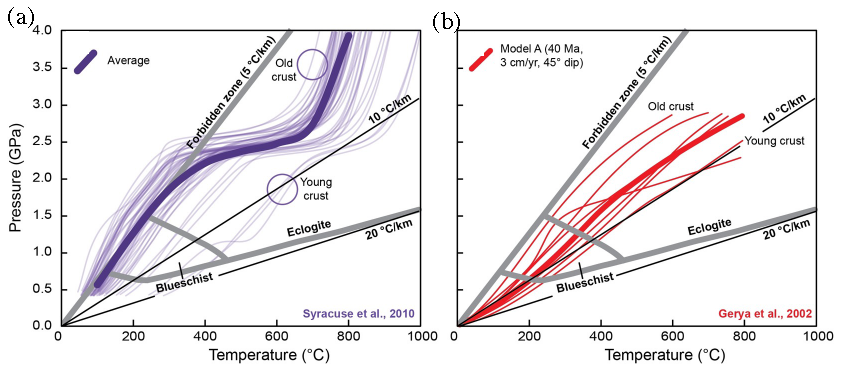
\includegraphics[width=6in]{global_subduction_eclogite.pdf}
    \caption[全球隱沒板塊頂部的預測P-T路徑圖,摘自\citet{penniston2015global}]{
    全球隱沒板塊頂部的預測P-T路徑圖,摘自\citet{penniston2015global}。圖中標示每公里5$^\circ$、10$^\circ$、20$^\circ$的地溫梯度與藍閃岩、榴輝岩溫壓位置。(a)來自\citet{syracuse2010global}的全球隱沒板塊P-T路徑圖(紫色線)。(b)來自\citet{gerya2002exhumation}的模型,紅色線代表不同年齡的隱沒板塊P-T路徑圖。
    }
    \label{fig::global_subduction_eclogite}
\end{figure*}

\section{平坦隱沒定義}\label{平坦隱沒定義}

地球內部的隱沒傾角在地域上變化極大。本研究對\textsl{slab 2.0} (\citealp{hayes2018slab2})全球模型中切出152條垂直於海溝的隱沒帶剖面(剖面位置參考自\citealp{Hu2020}),計算深度0-150 公里、距離海溝800公里內的隱沒帶傾角,以每5度為一間隔,獲得全球隱沒帶傾角分佈圖,如圖\ref{fig::number of tracsects}所示,全球只有大約$13\%$的隱沒帶傾角低於$20^\circ$。

目前學界並沒有明確的平坦隱沒定義,因此過去研究較少將低傾角隱沒帶與平坦隱沒分開討論,以往的數值模型多直接計算隱沒板塊在特定深度的斜率,一旦傾角低於特定值則視為平坦隱沒。
然而,隱沒板塊角度變化僅是最初步的隱沒帶特徵之一,隱沒帶中的幾何形狀更能展現隱沒帶的熱構造。
在上述的剖面中,將隱沒帶初步分成三類: 0-19$^\circ$、20-39$^\circ$、40-69$^\circ$,分別是為低傾角隱沒帶、正常隱沒帶與高傾角隱沒帶。
低傾角隱沒帶分別落在阿拉斯加、日本四國、卡斯卡迪亞(Cascadia)、墨西哥、新幾內亞以及安地斯隱沒帶上,\citet{schellart2020control}另外將低傾角隱沒帶分成兩種類型,在深度150 公里以上有兩個鉸鏈點(hinge)與三個鉸鏈點的隱沒板塊段,如圖\ref{fig::slab profile}所示。

\begin{figure*}[ht!]
    \centering
    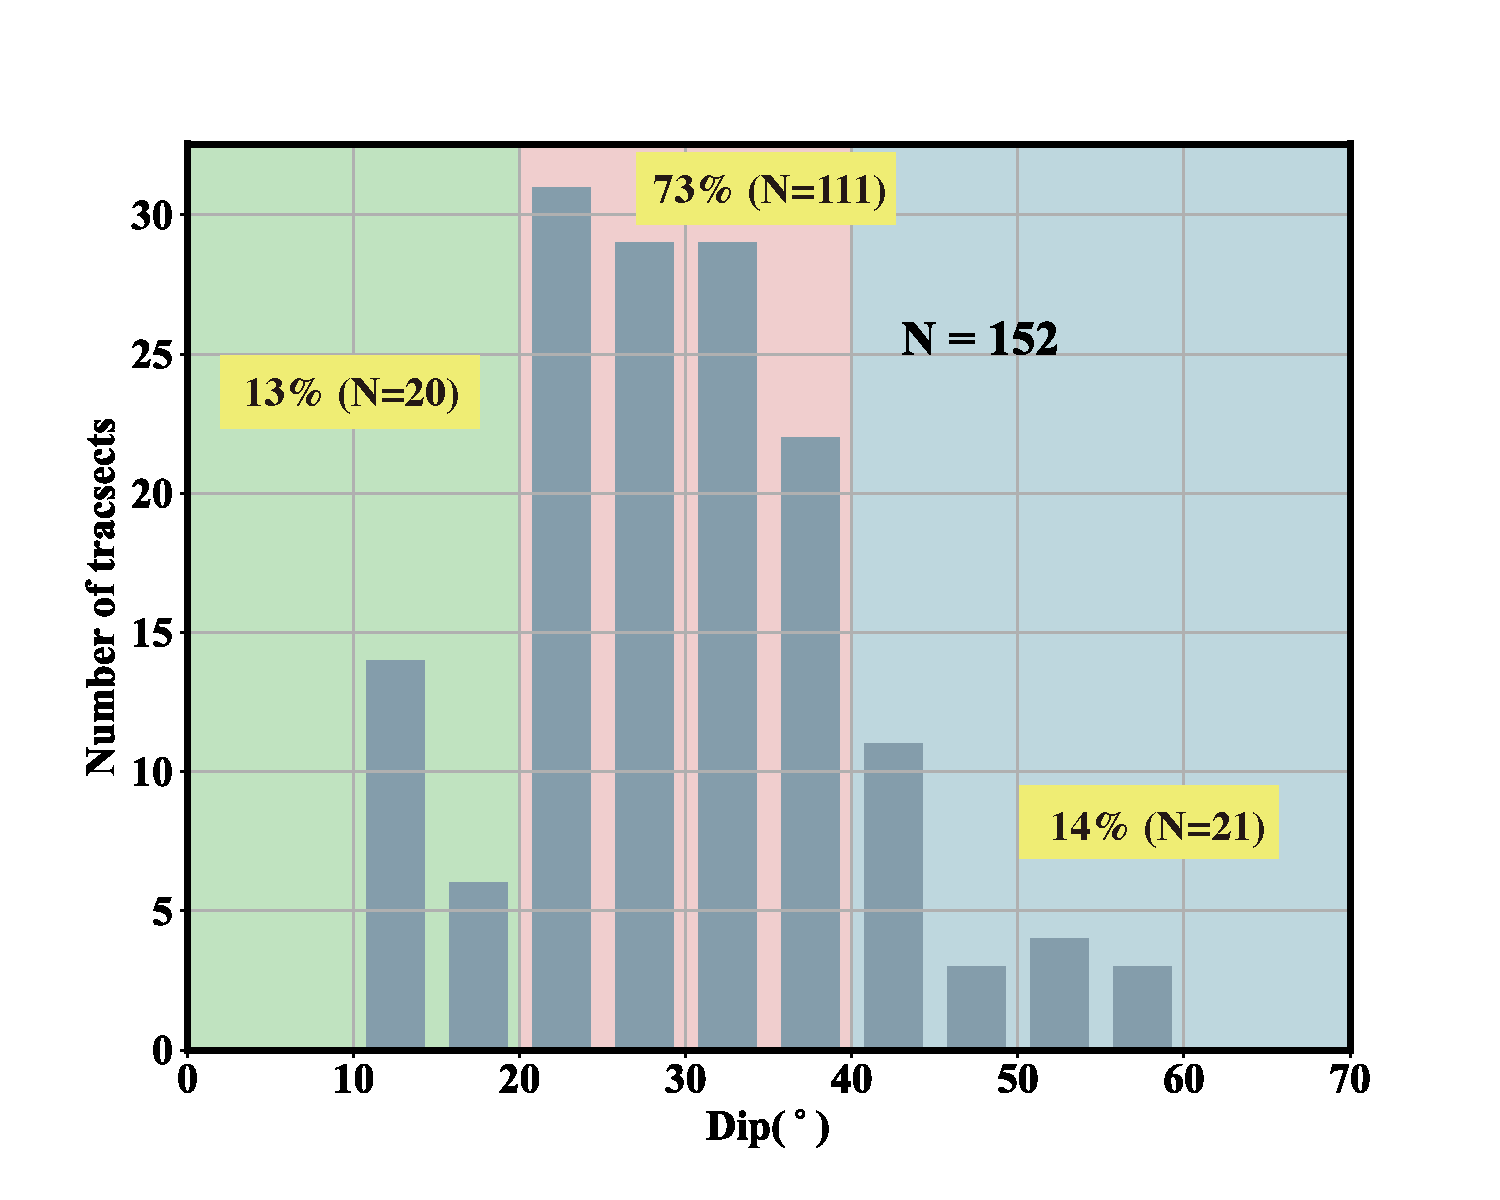
\includegraphics[width=4in]{chapter3_01.pdf}
    \caption[全球152條隱沒帶剖面傾角長條分布圖]{全球152條隱沒帶剖面傾角長條分布圖,其中綠底為隱沒剖面傾角低於20$^{\circ}$的剖面個數,佔整體13$\%$;粉紅底為剖面傾角介於20$^{\circ}$-39$^\circ$之間的剖面個數,佔整體$73\%$,粉藍底則為剖面傾角高於$40^\circ$的剖面個數,佔總體$14\%$。}
    \label{fig::number of tracsects}
\end{figure*}

\citet{schellart2020control}是少數將平坦隱沒與低傾角隱沒分開討論的研究,在他的定義中,相對於低傾角隱沒帶,大部分活躍的隱沒板塊具有一個鉸鏈點,接近海溝且下凹,如圖\ref{fig::slab profile}。
從圖\ref{fig::slab profile}可見,低傾角隱沒板塊會有兩個下凹鉸鏈點,第一個鉸鏈點接近海溝且呈現平緩不明顯的下凹,第二個鉸鏈點在距海溝幾百公里遠處,曲率明顯、板塊下凹進入深部地函,如圖\ref{fig::slab profile},阿拉斯加、卡斯卡迪亞、日本四國與新幾內亞等地區皆屬於此類。
另外在少數區域,隱沒板塊會有三個鉸鏈點,第一個鉸鏈點靠近海溝且下凹,第二個鉸鏈點深度較深且呈現上凹,被視為是平坦隱沒的開始端,在這兩個鉸鏈點中隱沒板塊傾角正常。
第三個鉸鏈點與第二個鉸鏈點深度相近,水平距離通常超過100公里以上,其曲率下凹的特徵代表著平坦隱沒的結束,平坦隱沒的距離與深度由第二與第三鉸鏈點所決定,如圖\ref{fig::slab profile}所示,智利、秘魯與墨西哥等地區屬於此類,在過去曾經被\citet{Manea2017}所討論。


\begin{figure*}[ht!]
    \centering
    \includegraphics[width=6in]{Slab_2.0_v1.pdf}
    \caption[slab 2.0 模型與四條參考剖面,改編自\citet{schellart2020control}]{slab 2.0 模型與四條參考剖面,改編自\citet{schellart2020control}。其中(a)為馬尼拉隱沒帶剖面,(b)為阿拉斯加隱沒帶剖面,(c)為加勒比板塊隱沒帶剖面,(d)為秘魯隱沒帶剖面。}
    \label{fig::slab profile}
\end{figure*}


然而由於過去研究對隱沒板塊鉸鏈點與曲率並沒有詳細定義,因此本研究並不採用上述的方式定義平坦隱沒,而是使用反曲點(Inflection point),方便後續對轉動力矩(見\ref{計算數值模型中的轉動力矩}節)進行比對,並且從數學面向來看更具有平坦(flat)的意義。
其中,反曲點的定義為連續曲線上穿越切線的點,亦即曲線二次微分等於0的點。
本研究將具有三個反曲點的隱沒段視為平坦隱沒,隱沒板塊曲線上除了具有兩個下凹特徵外,包含在兩側下凹隱沒中有一近乎平坦的隱沒段,有別於低傾角隱沒段的上下界深度落差可達50公里,其隱沒板塊在一固定深度幾乎維持水平狀態持續逾百公里以上。
為了確保數值模型中隱沒板塊是否符合平坦隱沒定義,本研究利用數學定義判斷平坦隱沒是否存在。
假設隱沒板塊為連續函數,令隱沒板塊方程式為$f(x)$, 其中$(x_{1},f(x_{1}))$, $(x_{2},f(x_{2}))$為x方向上最大的兩個反曲點(見圖\ref{fig::flat slab definition})。若為平坦隱沒,需同時滿足:

1. 最大兩個反曲點水平距離需大於100公里($\mid x_{1}-x_{2}\mid > 100 \ km$)。

2. 對整段隱沒板塊微分,其斜率的絕對值小於0.2之連續距離需大於50公里,該連續段稱為平坦隱沒之平坦段長度,其深度中位數稱為平坦段深度。

\begin{figure*}[ht!]
    \centering
    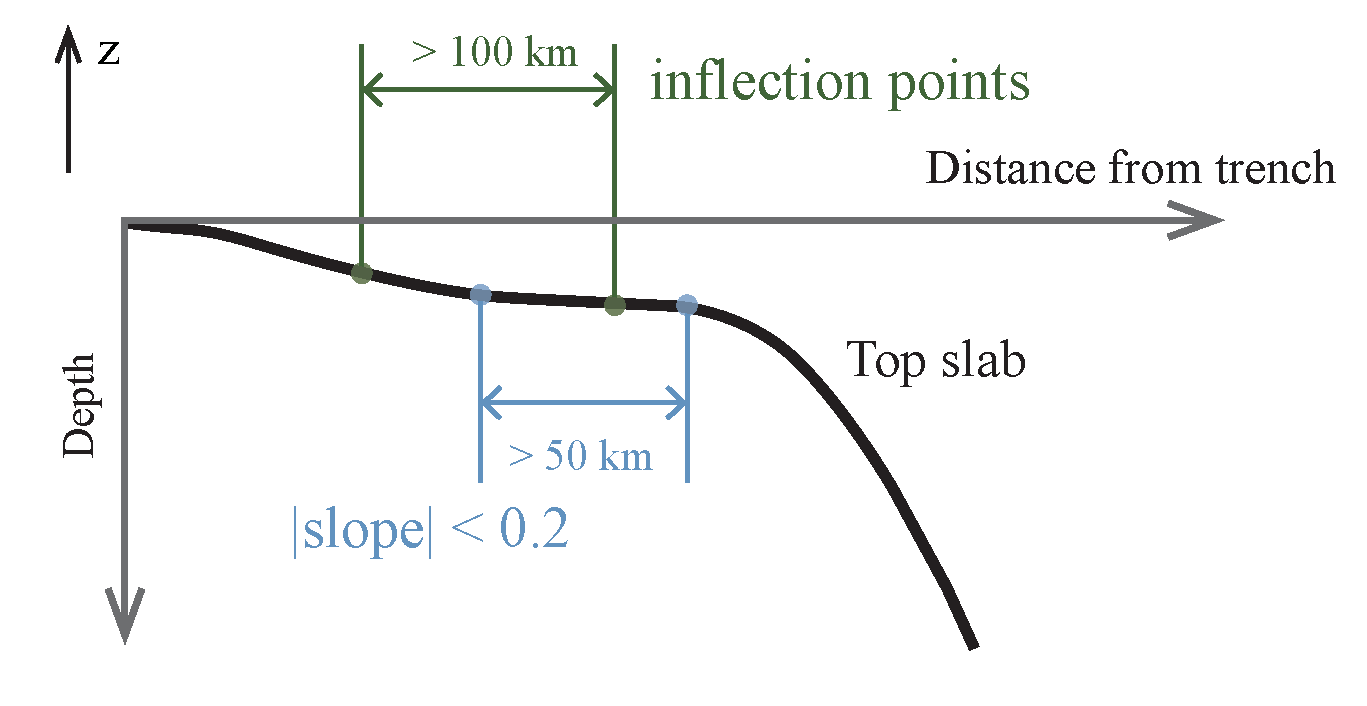
\includegraphics[width=6in]{flat_slab_definition.pdf}
    \caption[本研究中平坦隱沒的定義示意圖]{本研究中平坦隱沒的定義示意圖。綠色點表示隱沒板塊頂部上的反曲點,藍色點為隱沒板塊頂部上斜率絕對值小於0.2內最大連續範圍段的起點與終點。}
    \label{fig::flat slab definition}
\end{figure*}

如前所述,過往研究對平坦隱沒並沒有確切定義,絕大多數對平坦隱沒的判斷依據皆是以在固定深度範圍內隱沒板塊角度低於15-20度便視為平坦隱沒,然而這種定義除了無法分辨低傾角隱沒與平坦隱沒外,所選取的隱沒板塊深度範圍是另一種可變參數,結果較為發散。
重新定義平坦隱沒能夠用更具物理意義的方式觀察平坦隱沒在板塊運動中的各種動力影響。
藉由上述的定義方式,本研究重新分析152條隱沒剖面,結果表示只有科克斯板塊(Cocos plate)隱沒帶上的墨西哥區域與納茲卡板塊(Nazca plate)隱沒帶上的秘魯與智利區域有平坦隱沒的現象。

因此,接下來本研究以探討這三個區域的隱沒帶為主,其地理位置標示於圖\ref{fig::flat_slab_vol}的黃色框框中。

\begin{figure*}[hp]
    \centering
    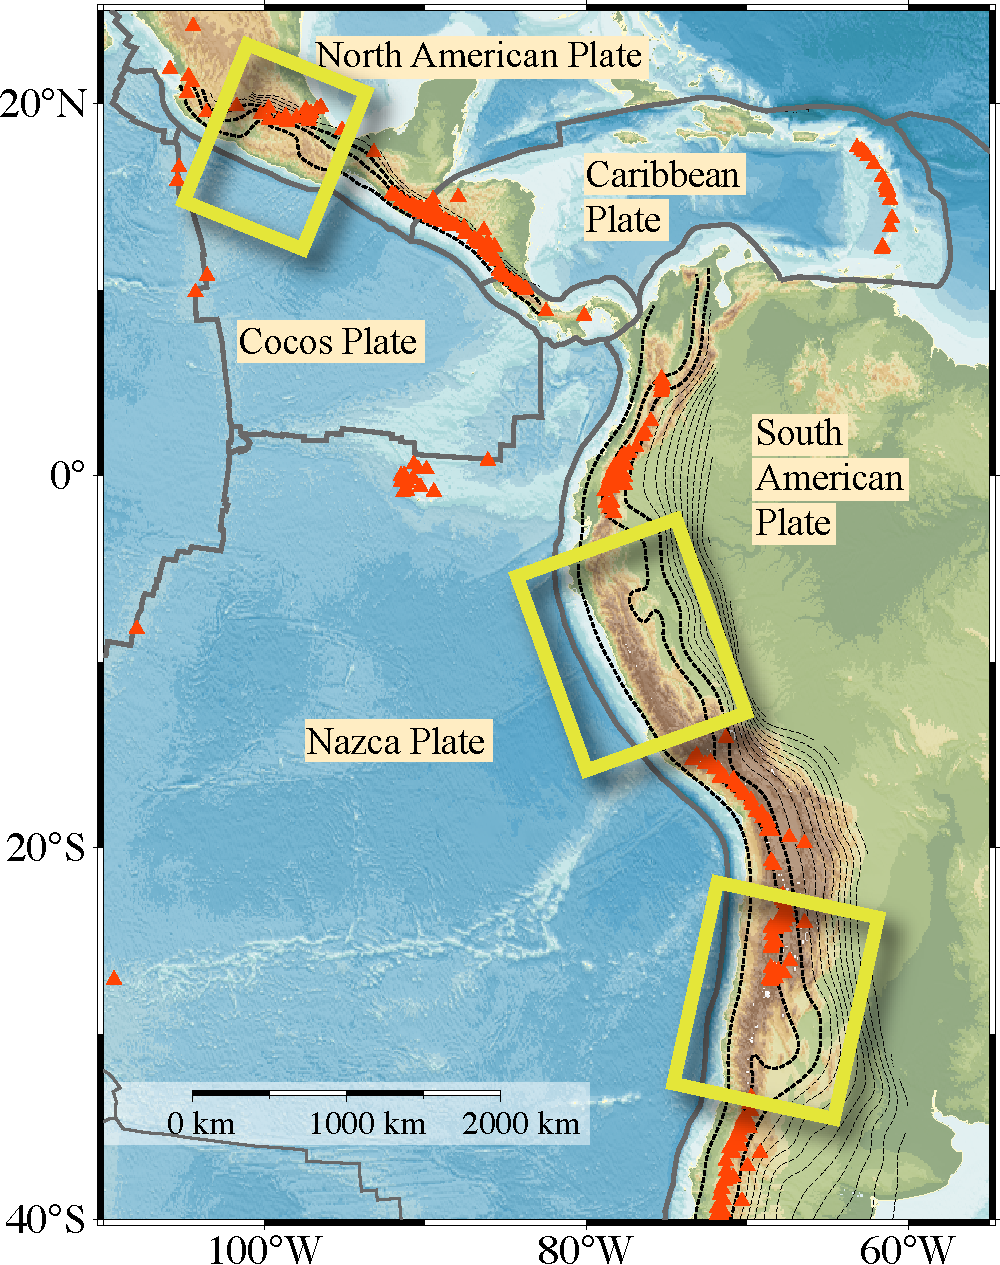
\includegraphics[width=6in]{flat_slab_vol_v1.pdf}
    \caption[研究區域板塊構造圖]{研究區域板塊構造圖,灰色實線為板塊邊界,資料來自\citet{bird2003updated},橘紅色三角形為火山分佈,資料來自\citet{venzke2013global},黑色虛線為每50公里深之板塊等深度線,其中50、100與150公里等深度線加粗,資料來自\citet{hayes2018slab2}。黃色框框圈起處為本研究所定義的平坦隱沒位置,由北到南分別位於墨西哥、秘魯與智利。
    }
    \label{fig::flat_slab_vol}
\end{figure*}

從物理的角度來看,造成隱沒板塊的傾角變化可以用力矩來解釋(\citealp{stevenson1977angle}),見圖\ref{fig::Torque}。
施加於隱沒板塊上的兩個轉動力矩分別為重力力矩(gravity torque)與動水壓力力矩(hydrodynamic pressure torque)(\citealp{McKenzie1969})。

重力力矩主要來自隱沒板塊與周遭地函的密度差。
同\ref{背景}所述,該密度差同時有化學與溫度上的影響: 玄武岩相變導致地殼密度增大,此為化學上之影響; 同時隱沒板塊溫度相對地函較低,導致海洋岩石圈密度較地函大,此為溫度上之影響。
由於重力(gravity force)指向地心,在圖\ref{fig::Torque}中,若假設海溝為轉動支點(fulcrum),則該隱沒系統之海洋岩石圈上任一點的重力效應,皆會造成順時針方向上的轉動。
而動水壓力力矩來自隱沒板塊下地函與隱沒板塊上地函楔(mantle wedge)的動水壓力差。
圖\ref{fig::Torque}中綠色線段為隱沒系統中假想的流線(streamline)。
相對於隱沒板塊下方的地函,隱沒過程中地函楔側之速度變化大,導致速度梯度大,容易產生低壓環境。
隱沒板塊下方的地函相對速度變化小,壓力相對高壓。
而為了平衡壓力,高壓會往低壓流動,此現象所產生的加速度稱為動水壓力(壓力梯度力),該力會垂直於隱沒板塊,且若壓力差越大,則動水壓力越大。
同樣假設海溝為轉動支點,這裡定義隱沒板塊上每個點所承受的動水壓力正向方向為朝地函楔為正,於是其所產生的正向動水壓力力矩於圖\ref{fig::Torque}中為逆時針轉動。
該轉動現象在看似對隱沒板塊產生往上吸的影響,因此動水壓力力矩又可稱為吸力力矩(suction torque)(\citealp{tovish1978mantle}),而動水壓力又可稱為吸力(suction force)。

\begin{figure*}[ht!]
    \centering
    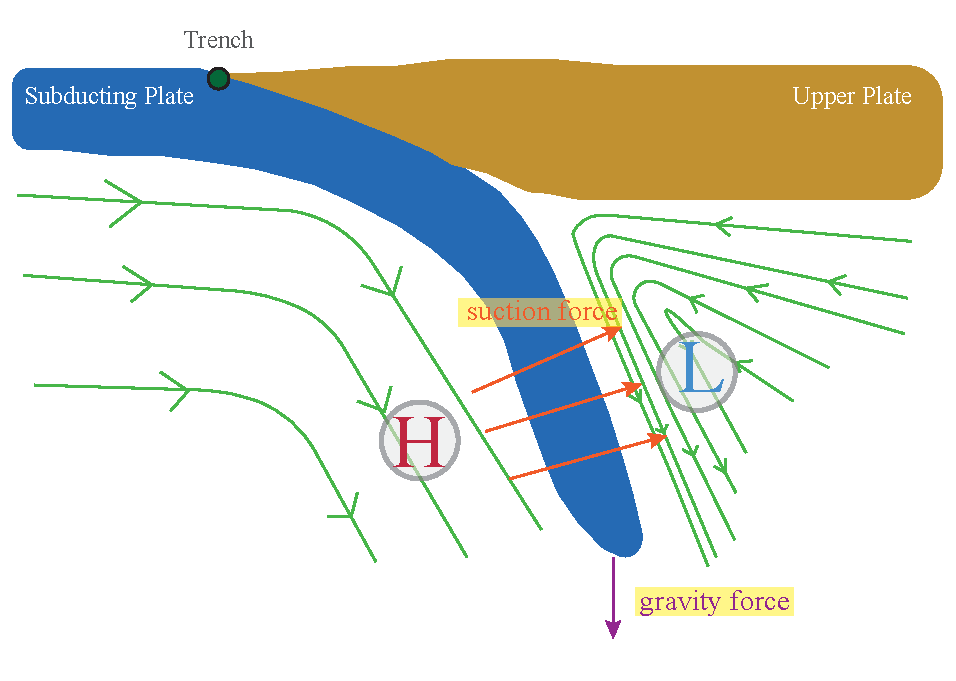
\includegraphics[width=6in]{torque_v3.pdf}
    \caption[隱沒系統中施加於隱沒板塊上的轉動力矩]{隱沒系統中施加於隱沒板塊上的轉動力矩,包含重力力矩與動水壓力力矩。綠色線為軟流圈(asthenosphere)中的假想流線,灰圓底紅字H代表高壓區,灰圓底藍字代表低壓區。假設海溝為支點,大於0之重力力矩在該系統中施予一順時針方向上的轉動,反之大於0之動水壓力力矩施予一逆時針方向上的轉動。
    }
    \label{fig::Torque}
\end{figure*}

隱沒系統的重力力矩直接與隱沒板塊有關,過去有不少數值模型改變隱沒板塊上的物質狀態形成平坦隱沒,例如,在隱沒板塊上放置一段增厚海洋地殼(\citealp{van2002role}; \citealp{Liu2016}; \citealp{Hu2016}等)、延後生成高密度的榴輝岩相或不生成榴輝岩相(\citealp{van2002role})、降低隱沒板塊整體密度(\citealp{Gerya2009})、設計斷掉的隱沒板塊(\citealp{Liu2016})等。
由於早期認為平坦隱沒的生成與隱沒板塊有直接關係,因此過去的數值模型研究在這方面已經相當豐富。

動水壓力力矩所牽扯到之因素較難約束,也較為複雜,例如上覆板塊的厚度、溫度、強度(strength)、受力狀態等,以及地函中的黏滯度(viscosity)、板塊聚合速率(convergent rate)、岩漿庫(magma chamber)位置與大小等,都有可能是影響動水壓力力矩大小的原因。
過去數值模型研究中,試圖以多種模型設定探討隱沒系統中動水壓力力矩增加的可行性,包含克拉通(craton)的存在(\citealp{Manea2012Chile}; \citealp{Liu2016}; \citealp{Hu2016})、隱沒帶中脫水作用所產生的低黏滯度區域(\citealp{Manea2007})與上覆板塊的溫度構造(\citealp{Thermal2012})。

\section{平坦隱沒的數值模型}\label{平坦隱沒的數值模型}
\subsection{隱沒的洋脊或海洋高原存在爭議}\label{隱沒的洋脊或海洋高原存在爭議}
早期概念模型研究將平坦隱沒與隱沒的洋脊(oceanic ridge)或海洋高原(oceanic plateau)的時空關係相連結(\citealp{pilger1981plate}; \citealp{henderson1984mesozoic}; \citealp{Gutscher2000A}; \citealp{gutscher2002andean}),\citet{Gutscher2000A}利用地震分布與早期地震波層析成像勾勒出隱沒的印加高原(Inca Plateau)與納茲卡中洋脊(Nazca Ridge)現今地下構造位置,成功與祕魯平坦隱沒的位置相對應(見圖\ref{fig::Gutscher_2000_ridge})。
對此,\citet{Gutscher2000A}認為海洋地殼上海洋高原與洋脊的存在可能會導致總體密度較低、浮力較大,
如\ref{背景}節所述,主要造成板塊隱沒的驅動力是隱沒後海洋地殼上的榴輝岩。
榴輝岩的密度高於地函,因此隱沒板塊可以產生足夠大的板塊拉力(slab pull)。
相比之下,海洋地殼的玄武岩質密度低於地函,故與普通的海洋地殼相比,較厚的海洋地殼在還沒有相變成榴輝岩之前密度確實較低,因此在隱沒初期能造成低傾角隱沒發生。
冷又厚的海洋岩石圈額外提供較低溫環境,導致榴輝岩化作用時間較長,於是系統中高密度物質體積較周遭其餘隱沒板塊小,促使平坦隱沒生成。

\begin{figure*}[htp]
    \centering
    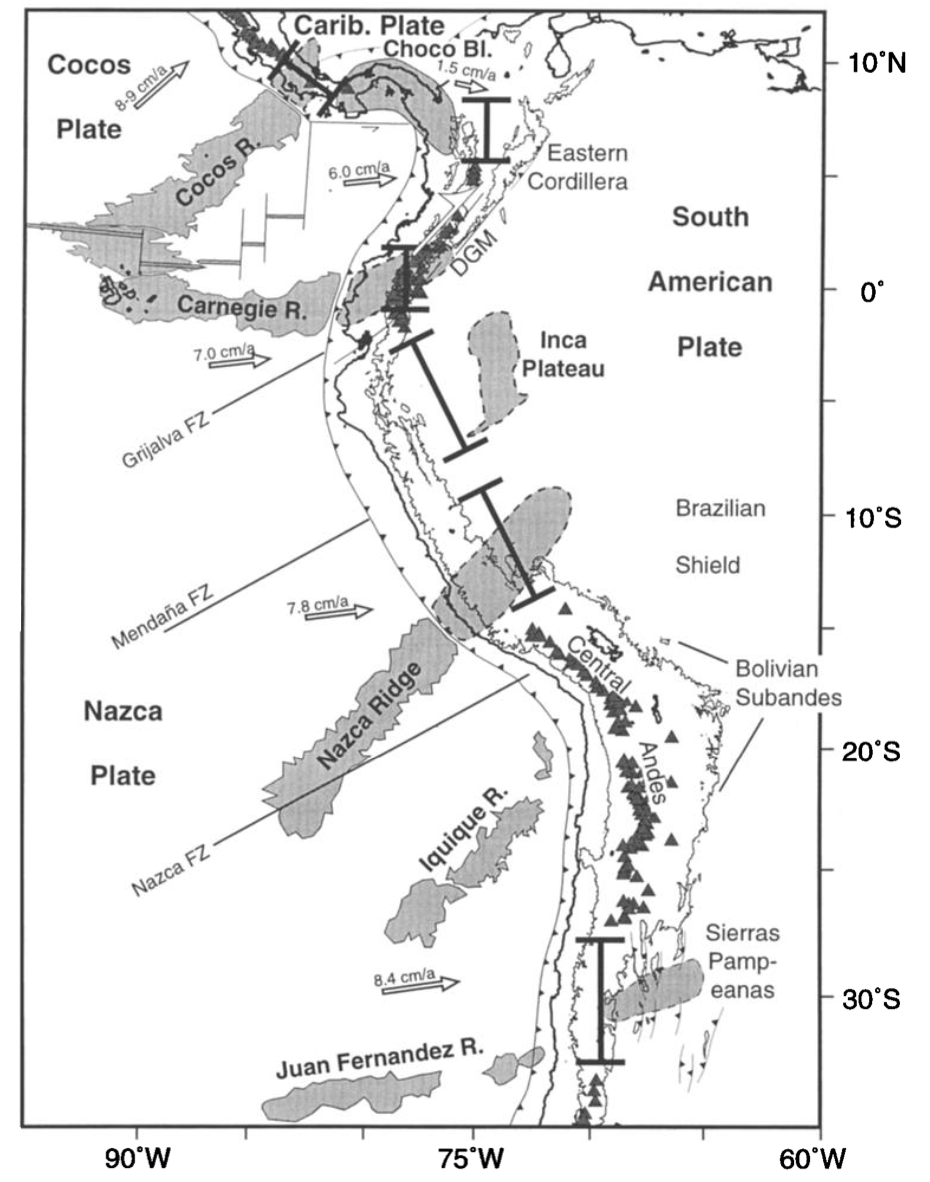
\includegraphics[width=6in]{Gutscher_2000_ridge.png}
    \caption[南美洲板塊構造圖,摘自\citet{Gutscher2000A}]{南美洲板塊構造圖,摘自\citet{Gutscher2000A}。粗黑線標出平坦隱沒段,灰色陰影區標示隱沒的海洋高原與洋脊,三角形為活動火山。板塊聚合速率由白色箭頭標出,參考自\citet{demets1990current}。
    }
    \label{fig::Gutscher_2000_ridge}
\end{figure*}

最早的平坦隱沒數值模型為\citet{van2002role} (見圖\ref{fig::van2002}),其利用二維尤拉笛卡爾座標熱化學數值模型,在海洋地殼上方增加一寬400公里、厚18公里的海洋地殼。
為了驗證\citet{Gutscher2000A}所提出的玄武岩相變延遲,\citet{van2002role}考慮成分隨時間的變化項,使用額外設定控制玄武岩相變成榴輝岩的延遲時間,為增厚的海洋地殼提供較大的浮力。
其結果表明若僅包含增厚的海洋地殼不足以形成平坦隱沒,需要同時有快速的板塊聚合速度才能觸發平坦隱沒的形成。
然而無論觀測上與實驗上對平坦隱沒的玄武岩相變延遲皆沒有太充足的證明。

\begin{figure*}[hb!]
    \centering
    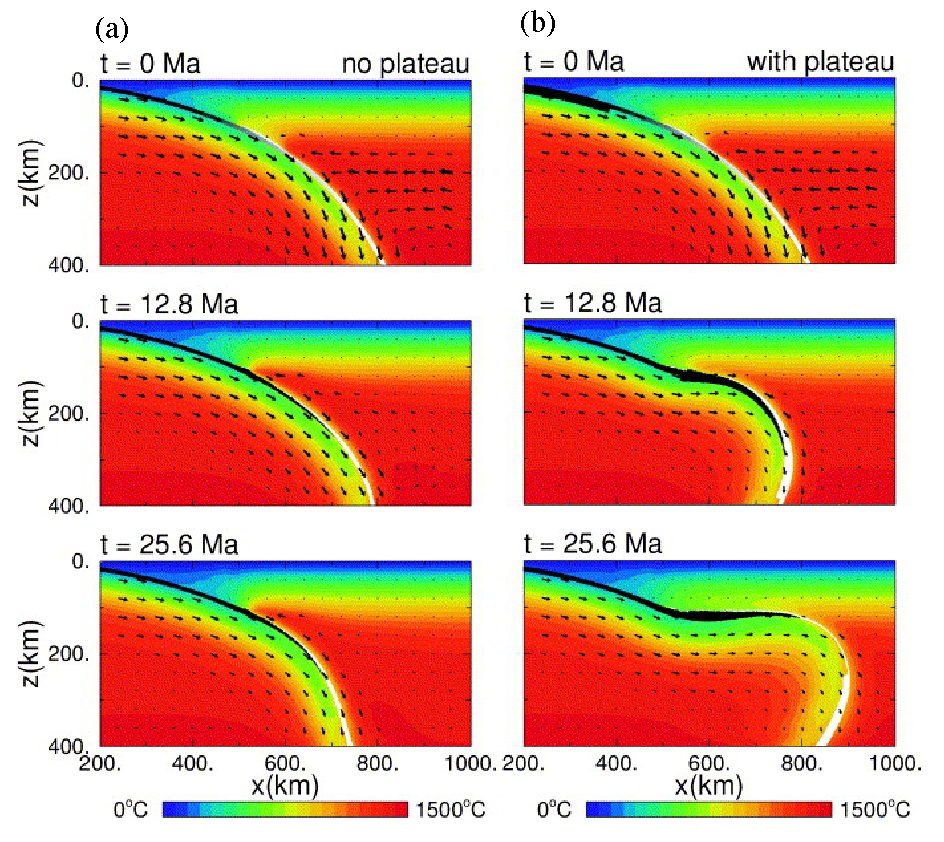
\includegraphics[width=6in]{van2002.pdf}
    \caption[正常的隱沒帶與包含海洋高原的隱沒帶隨模型時間變化,摘自\citet{van2002role}]{正常的隱沒帶(左)與包含海洋高原的隱沒帶(右)隨模型時間變化,摘自\citet{van2002role}。黑白區域繪出海洋地殼的化學成分從玄武岩(黑)到榴輝岩(白)的變化。水平軸為與海溝的距離,背景顏色為溫度。
    }
    \label{fig::van2002}
\end{figure*}

\citet{Gerya2009}使用二維尤拉笛卡爾座標模型(I2VIS)探討平坦隱沒帶與洋脊隱沒的關係,該模型包含脫水作用、部分熔融與地表高程變化。
為了模擬納茲卡洋脊的存在,模型中隱沒板塊上存在一200公里寬、18公里厚的玄武岩洋脊隱沒進入上覆板塊之下(見圖\ref{fig::Gerya2009})。
模型結果顯示平坦隱沒的形成與洋脊的存在與否無關,只要是密度異常低的海洋岩石圈(見圖\ref{fig::Gerya2009}a)皆有利於其形成。
並且,洋脊的存在與岩漿作用是否活躍也無關,當平坦隱沒存在,高溫的地函楔被隱沒板塊閉合,岩漿活動大量減少,有別於在相同情況下沒有平坦隱沒的隱沒帶(見圖\ref{fig::Gerya2009}b)。
值得一提的是,該模型並沒有考慮玄武岩至榴輝岩的相變過程,平坦隱沒在地殼密度低的情況下發育。

\begin{figure*}[ht!]
    \centering
    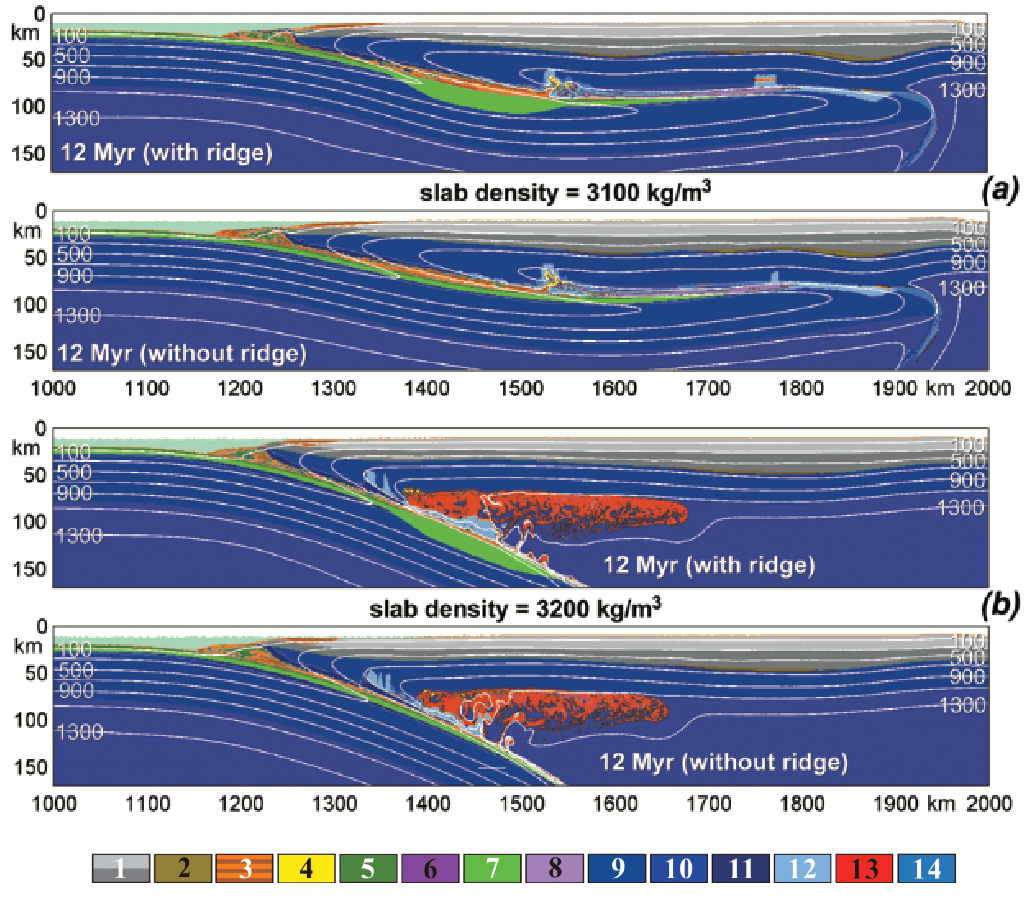
\includegraphics[width=6in]{Gerya_final.pdf}
    \caption[\citet{Gerya2009}平坦隱沒模型結果]{\citet{Gerya2009}中平坦隱沒模型於第12個百萬年的結果。圖組(a)與圖組(b)分別為隱沒海洋地函岩石圈密度為3100 kgm$^{-3}$與3300 kgm$^{-3}$的結果。(a)上圖與(b)上圖為包含洋脊隱沒的模型,(a)(b)下圖為不包含洋脊的模型,圖中白線為等溫線。其中,顏色代表不同岩相: 1、2 = 大陸地殼、3、4 = 沉積物、5、6 = 玄武岩、7、8 = 輝長岩、9、10 = 無水地函、11 = 蛇紋岩、12、13、14 = 含水地函。
    }
    \label{fig::Gerya2009}
\end{figure*}

\citet{Liu2016}利用二維任意拉格朗日-尤拉模型(SOPALE)討論過去拉臘米造山運動(Laramide orogeny)時期($\sim$80–50百萬年前)法拉龍板塊(Farallon plate)發生的平坦隱沒事件。
模型的隱沒板塊上設定一段400公里寬的海洋高原,包含18公里厚的增厚玄武岩海洋地殼與36公里厚的斜輝橄欖岩(harzburgite)地函岩石圈。
該模型也假設海洋高原上的玄武岩並不會發生榴輝岩相變,並且斜輝橄欖岩地函岩石圈密度比周遭地函低100 kg$\cdot$m$^{-3}$。
研究結果表明增厚海洋高原與快速的聚合板塊是平坦隱沒發育的必要條件。
模型中同樣沒有考慮玄武岩至榴輝岩相變過程。

上述研究中,將模型加入增厚海洋地殼的結果雖然都能讓平坦隱沒發育,但皆存在兩個問題。
第一,上述文獻中所有模型皆是二維模型,這意味著在第三維上有無限延伸的增厚海洋地殼,於是,增厚洋殼能在二維假設下提供足夠大的浮力,然而現實中增厚洋殼能造成的浮力效應應遠小於二維模型中的結果。
\citealp{florez2019impact}在三維模型中證明了這一點,他們的研究結果表明若將現在自然界中最大的洋脊隱沒進入地函中,其所提供的浮力也只會造成海洋板塊傾角減少原先的10度。
除此之外,浮力效應的量值是另一個潛在問題。
增厚的海洋地殼之所以能為隱沒板塊提供浮力,是因玄武岩的密度小於橄欖岩地函。
隱沒過程中,儘管玄武岩與地函橄欖岩的密度差不變,增厚的海洋地殼相對於正常海洋地殼擁有更大體積的低密度物質,因此能產生更大的浮力。
不過一旦玄武岩相變至榴輝岩相,大體積榴輝岩所造成的重力效應將會導致隱沒板塊重力力矩急劇增大,反而會抑制平坦隱沒的發育。
這緊接著點出後續問題。
第二,過去研究針對玄武岩至榴輝岩相變過程並沒有完善的解釋,\citealp{van2002role}所使用的相變延遲現象無法用實驗所證明,而剩餘研究皆沒有考慮此相變過程。
對此,上述對重力力矩減少的原因事實上難以與自然界的觀測吻合。


\subsection{實現數值模型中增加的地函動水壓力力矩}
\citealp{tovish1978mantle}計算隱沒帶中的角流(corner flow)指出非牛頓流體的地函可以產生極大的地函流吸力(mantle flow suction force),此時動水壓力力矩足夠抵抗重力力矩,形成平坦隱沒。
不過正如\ref{背景}節所述,不同於重力力矩直接與隱沒板塊物理特徵有關,隱沒系統中能夠影響動水壓力力矩的因素難以被量化與控制,因此過去討論動水壓力力矩的數值模型研究較少。

\citealp{Manea2007}使用二維模型CitcomS研究隱沒帶中脫水作用、地函黏滯度與動水壓力對隱沒板塊幾何的影響。
模型的地函楔中假設隱沒板塊脫水作用會產生一近似梯型低黏滯度區,詳見圖\ref{fig::Manea2007}。
他們改變圖\ref{fig::Manea2007}中橘紅色區域的黏滯度,發現較低的黏滯度可以增加地函楔中的壓力,導致板塊兩側的壓力差減少,大幅度減少隱沒系統的地函流吸力。
該研究指出過去\citealp{tovish1978mantle}的解析解研究並沒有考慮隱沒帶中的脫水作用影響,這意味著過去計算隱沒板塊力矩時,很可能高估地函吸力的量值。
%數值模型雖然可以透過測試地函黏滯度量值獲得平坦隱沒模型,然而黏滯度量值大範圍的不確定性難以證明模型的真實性。

\begin{figure*}[ht!]
    \centering
    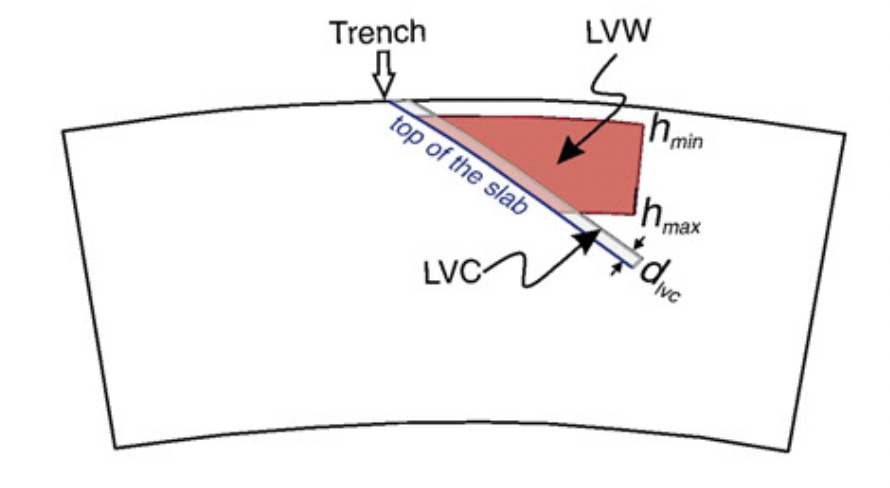
\includegraphics[width=3in]{Manea2007.png}
    \caption[\citealp{Manea2007}模型中所設定的低黏滯度近似梯形區與低黏滯度通道區域]{\citealp{Manea2007}模型中所設定的低黏滯度近似梯形區(LVW, low viscosity wedge)與低黏滯度通道(LVC, low viscosity channel)區域,表示隱沒帶的脫水作用對地函楔造成的影響。其中h$_min$、h$_max$、d$_lvc$皆為模型中可調整的參數,用以控制低黏滯度近似梯形區與低黏滯度通道的範圍與深度。}
    \label{fig::Manea2007}
\end{figure*}

\citealp{Thermal2012}利用包含牛頓流體(diffusion creep)與非牛頓流體(dislocation creep)的複合流變學不可壓縮流二維模型,討論上覆板塊的溫度構造與平坦隱沒的關係,模型中海溝位置不隨時間改變。
他們的結果認為冷硬的大陸岩石圈可以促使隱沒板塊角度變低,同時他們使用解析解的方式計算模型中重力力矩與動水壓力力矩的大小。
該研究結論支持平坦隱沒不是一個穩態(steady-state)狀態,平坦隱沒只有在隱沒作用初期、隱沒板塊長度不到400公里時會出現。
不過這與現生的平坦隱沒形成時間抵觸,無論是智利、秘魯或墨西哥的平坦隱沒都不是隱沒初期的構造,三個地區的隱沒帶已經持續超過180 Ma(\citealp{Schellart2021}),皆是近期(<15 Ma)才有平坦隱沒事件發生(\citealp{chen2019southward}; \citealp{hu2021southward})。

\citealp{o2009subduction}利用有限元素法模型計算增厚大陸岩石圈對地函楔角流(mantle wedge corner flow)的影響,進而計算地函楔動水壓力的大小。
他們的結果顯示若大陸岩石圈具有250公里厚且寬度200公里的山根(root)時,地函楔中的角流降低,動水壓力力矩可增加至原先無山根模型的四倍。
儘管他們的模型研究並沒有包含平坦隱沒,但大陸岩石圈山根影響動水壓力力矩的概念成功開啟往後動水壓力力矩的數值模型研究,為後續平坦隱沒數值模型的研究提供新的方向。

\citealp{Manea2012Chile}利用三維模型模擬過去30個百萬年來智利區域的隱沒帶動態行為,邊界條件與\citealp{Thermal2012}幾乎相同。
模型開始先是普通的隱沒帶模型,在隱沒帶發育成熟後,額外施加一段邊界條件強迫智利海溝後撤,他們發現海溝後撤能夠施加給隱沒板塊的地函流吸力,不過該吸力量值不足以讓巨大厚重的海洋板塊變平坦。
爾後他們效仿\citealp{o2009subduction}的模型設計,嘗試將南美洲大陸數個古老克拉通(craton)地塊加入模型中。
利用改變上覆板塊溫度梯度,讓模型的上覆板塊厚度增厚,此初始設定代表冷硬的克拉通構造,該地質構造成功讓地函楔角流下降,隱沒帶系統的動力壓力增加,平坦隱沒得以順利形成,見圖\ref{fig::Manea 2012}。
因此他們得出的結論是需要同時有海溝後撤與克拉通的存在才會觸發平坦隱沒,這是首次在不更改隱沒板塊狀態、僅利用增加動水壓力產生的平坦隱沒模型。
他們的模型中沒有考慮地殼與地函的密度差,也沒有考慮任何相變過程。
隨後\citealp{Liu2016}效仿同樣的概念,將過去普遍認為存在於北美岩石圈西部下方的科羅拉多高原山根(Colorado Plateau)放入模型中,模擬法拉龍板塊平坦隱沒演化。
然而他們的研究表示克拉通或山根的存在只是加快平坦隱沒的形成,但真正觸發平坦隱沒的機制是增厚且沒有榴輝岩相變的海洋地殼,亦即動水壓力力矩對隱沒帶的影響並不大。
\begin{figure*}[ht!]
    \centering
    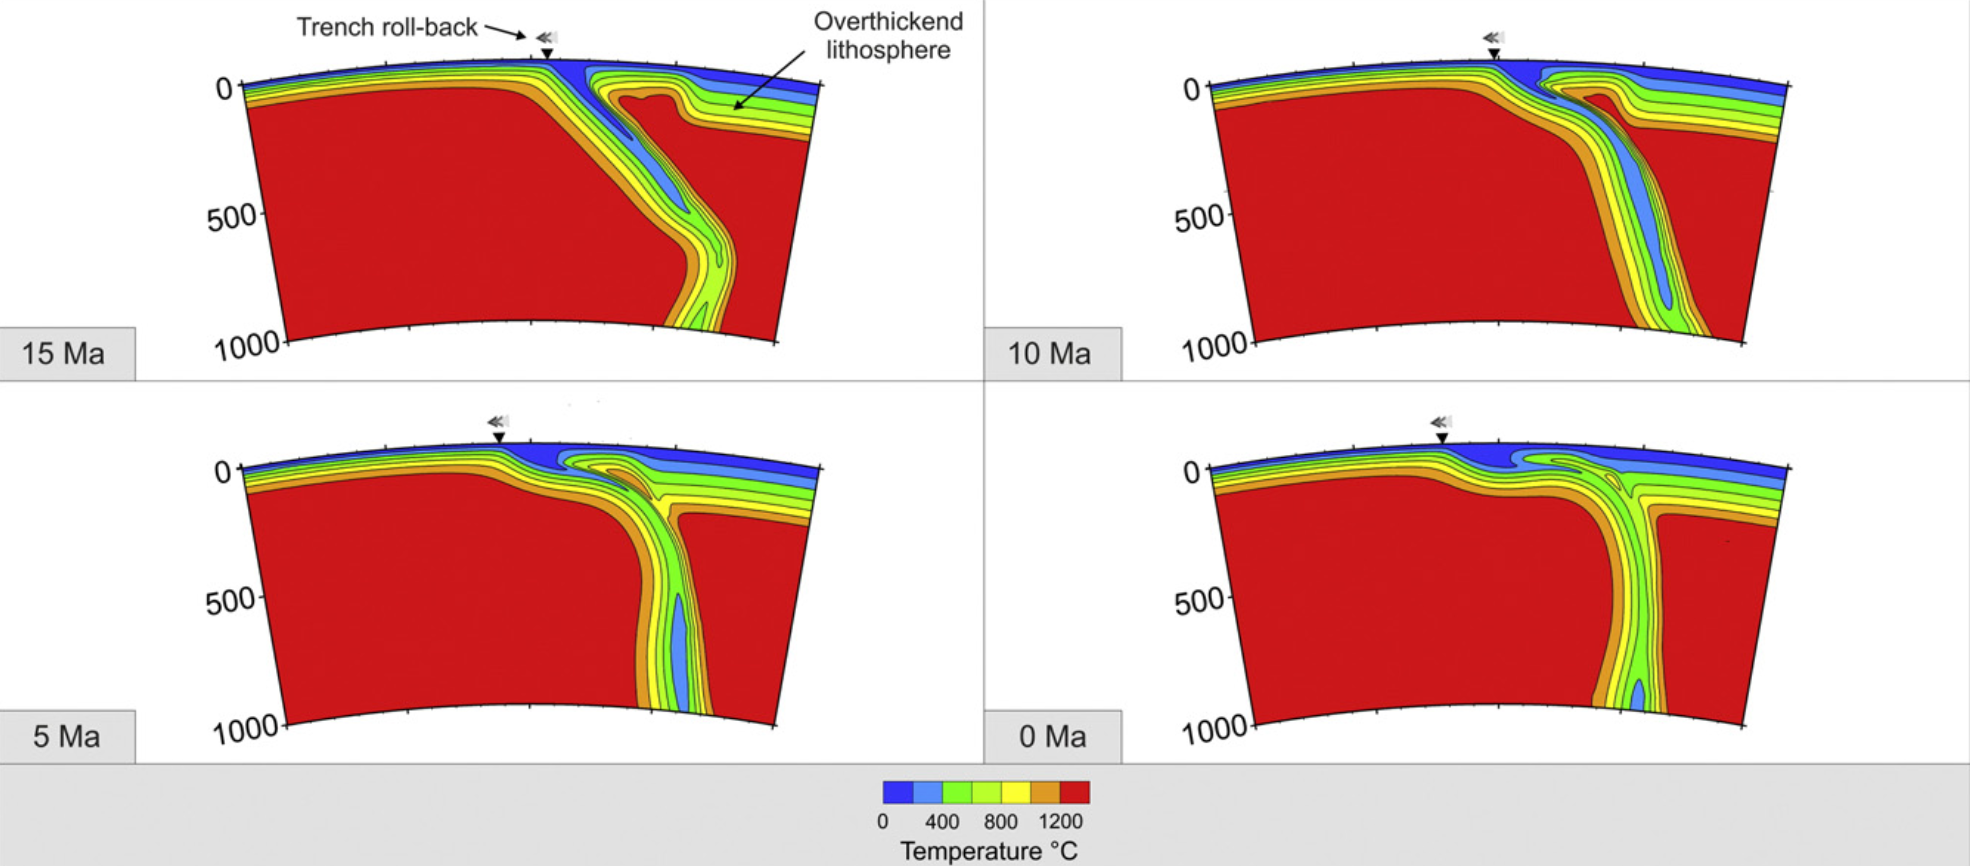
\includegraphics[width=6in]{Manea 2012.png}
    \caption[\citealp{Manea2012Chile}中的智利平坦隱沒模型]{\citealp{Manea2012Chile}中的智利平坦隱沒模型,模型中同時加入海溝後撤邊界條件與增厚大陸岩石圈可以讓平坦隱沒發育。模型背景顏色為溫度。
    }
    \label{fig::Manea 2012}
\end{figure*}

\citealp{Hu2016}重複與\citealp{Manea2012Chile}同樣的實驗,使用三維模型CitcomS模擬阿他加馬海溝(Atacama Trench, or Peru–Chile Trench)於45個百萬年以來隱沒帶的演化。
這次他們將觀測資料當作模型邊界條件,逐一分析海溝後撤、海洋高原隱沒與克拉通山根的存在對模型的影響,用以探討影響平坦隱沒形成的關鍵原因。
模型加入克拉通後,隱沒板塊傾角有降低的趨勢,不過並克拉通的影響不足以形成平坦隱沒,僅能視為低傾角隱沒。
隨後模型加入隱沒的海洋高原,隱沒傾角在區域(local)上顯著降低,表明隱沒的海洋高原才是平坦隱沒發育的主因。
故動水壓力力矩與重力力矩對平坦隱沒發育的角色仍然存在分歧。

\section{研究動機}\label{研究動機}
最簡單直接的平坦隱沒概念模型可以透過改變隱沒系統的重力力矩達成,尤其是早期的隱沒洋脊理論,然而過去動力學數值模型研究針對玄武岩至榴輝岩相變過程並沒有完善的物理機制解釋。
相較於隱沒帶中重力力矩的直觀性,動水壓力力矩增大的條件與其對隱沒帶造成的影響較難以用單一的地質構造或特性約束。
近年來地球動力學數值模型除了為地球內部構造提供物理約束外,也開始量化各種自然現象對岩石造成的物理特性改變,包含岩漿作用與脫水作用等。
尤其動水壓力力矩對隱沒系統的影響還沒有完全成熟,而這些較為複雜的地球內部作用或許可以為動水壓力力矩與隱沒帶構造的關係提供額外資訊。

過去研究還有另一個隱性問題,上述所有數值模型皆是模擬南美洲區域的隱沒帶。
對本研究所定義的平坦隱沒(詳見\ref{平坦隱沒定義}節),目前世界上只有墨西哥、秘魯與智利有平坦隱沒的現象。
而過去研究皆是以南美洲的秘魯與智利的平坦隱沒當作模型藍本,少部分考量法拉龍板塊的平坦隱沒事件,值得一提的是,目前尚未有任何墨西哥平坦隱沒的數值模型被提出。
在墨西哥,隱沒板塊上沒有任何隱沒海脊的紀錄,上覆板塊也沒有任何克拉通存在的證據,因此墨西哥的平坦隱沒確切原因更是沒有明確方向。

本研究將著重在探討動水壓力力矩在哪些環境下會發生改變,並且在考慮玄武岩至榴輝岩相變的過程下模擬平坦隱沒的發育,此外,本研究期待能利用數值模擬墨西哥平坦隱沒,填補過去尚未成熟的平坦隱沒機制。
接下來會針對各個平坦隱沒區域的觀測資料進行文獻回顧,包含納茲卡隱沒帶的秘魯、智利平坦隱沒區域以及科克斯隱沒帶上的墨西哥平坦隱沒。


\section{秘魯與智利隱沒帶的地球物理觀測}\label{秘魯與智利隱沒帶地球物理觀測}
\citet{barazangi1976}利用南美洲區域震源位置資料判斷秘魯與智利下方的隱沒板塊處於水平狀態,由於南美洲沿岸的地震事件數目多,可藉由垂直海溝剖面的班尼奧夫帶(Benioff seismic zone)很好的勾勒出隱沒板塊的角度與形狀。

不過秘魯與智利區域的地震測站並不多,導致過去並沒有太多地區性的地震層析成像研究。
\citet{Ma2014}是第一個針對秘魯區域的速度構造研究,他們的結果展示秘魯平坦隱沒最南段的表面波層析成像(surface wave tomography)。
隨後\citet{Ma2015}利用接收函數判斷秘魯平坦隱沒上方的莫荷面(Moho),再配合\citet{Ma2014}的層析成像結果,獲得秘魯平坦隱沒板塊上的構造,如圖\ref{fig::Peru_tomography}。
隱沒板塊的平坦段約在距海溝100公里處,深度落在80-100公里之間,並且平坦段並非呈現水平,而是有上凹又下凹的構造,平坦段長度大約350公里。
他們的結果表明秘魯的莫荷面與隱沒板塊的深度側向變化非常接近,可能暗示著該區域有強烈的板塊間吸力。
此外,他們觀察到在平坦隱沒距海溝較近處有高速的地函岩石圈(mantle lithosphere),V$_S$可達到4.5 km/s,該研究解釋為乾冷的岩石圈,見\ref{fig::Peru_tomography}下圖深橘色區段。
直到距離海溝350公里後,快速的地函岩石圈V$_S$降低成4.2-4.3 km/s左右,該速度是正常地函岩石圈的速度,他們解釋,可能是隱沒板塊上的物質直到距離海溝350公里後才發生脫水。

\begin{figure*}[ht!]
    \centering
    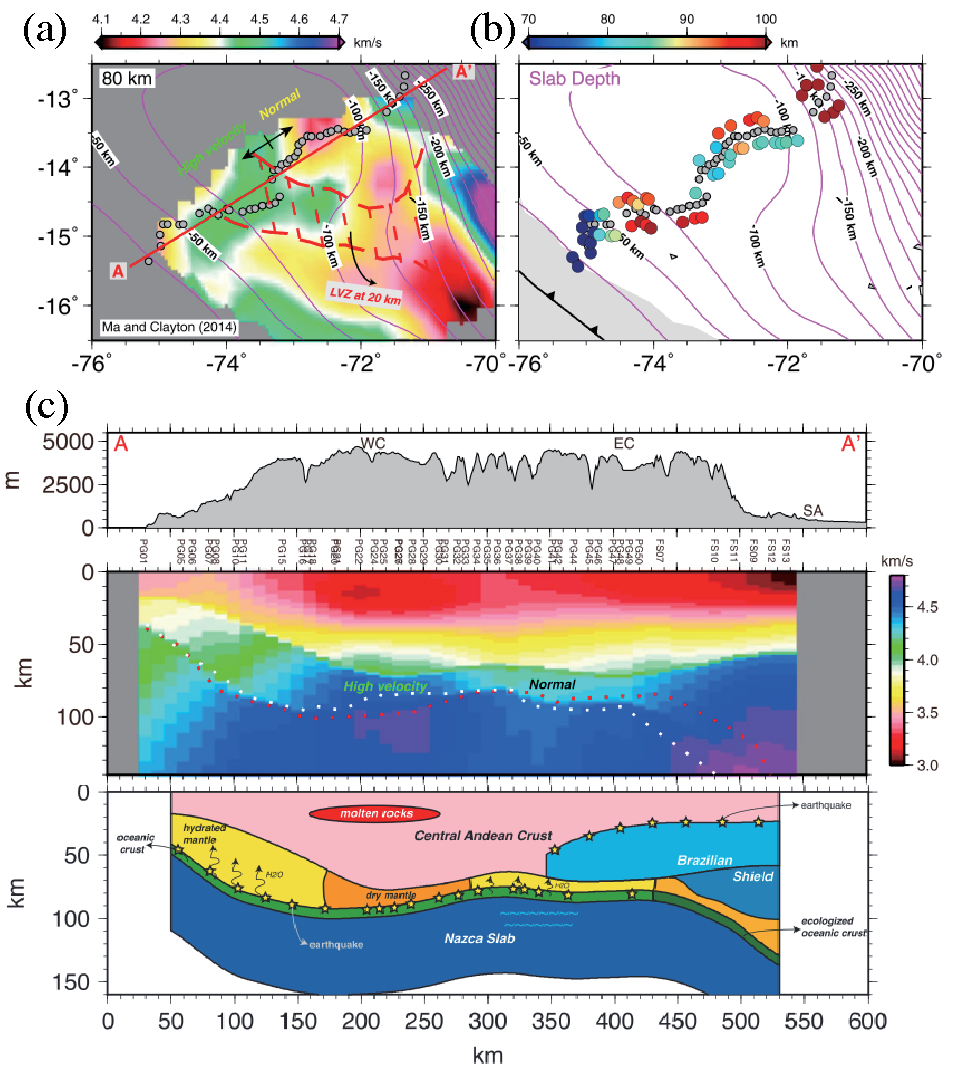
\includegraphics[width=5in]{Peru_tomography.pdf}
    \caption[秘魯平坦隱沒南段地震學研究結果與解釋圖,摘自\citet{Ma2015}]{秘魯平坦隱沒南段地震學研究結果與解釋圖,摘自\citet{Ma2015}。(a)深度80公里的V$_{SV}$速度構造,來自\citet{Ma2014}。圖中左上方標示高速地函岩石圈與正常地函岩石圈的分界。紅色虛線標示出於20公里深的低速帶範圍,該低速帶被解釋為熔融區。粉紅色線為板塊等深度線。紅色實線為圖(C)中AA'剖面位置。灰色點為該研究所使用的側站位置。(b)板塊等深度圖,各顏色點為接收函數轉換波的地殼入射點,顏色代表不同深度。灰色點為該研究所使用的側站位置。(c)最上圖為AA'剖面地形,中圖為AA'剖面V$_{SV}$速度構造圖,白色點與紅色點分別為接收函數於西北地震事件群與東南地震事件群所獲得之板塊深度。最下方為AA'剖面結構卡通圖,大陸與海洋莫荷面深度來自圖(b)中的結果。
    }
    \label{fig::Peru_tomography}
\end{figure*}

\citet{Marot2014}利用三維區域地震層析成像與衰減模型討論了圖\ref{fig::Chile_geology_profile}中智利平坦隱沒與智利南段正常隱沒帶的構造差異。圖\ref{fig::Chile_geology_profile}c、圖\ref{fig::Chile_geology_profile}d分別為平坦與正常的隱沒帶地震事件剖面,可見在平坦隱沒板塊區域的地震事件遠多於正常的隱沒板塊區域。他們的結果顯示平坦段在深度25、50與70公里處各有一段低速帶,如圖\ref{fig::Chile_tomography},在透過熱模型與速度對比後,他們認為低速帶可能是板塊脫水區,這導致蛇紋岩化橄欖岩在局部生成,正常的隱沒板塊段同樣也有類似的速度構造結果。
經過速度與熱構造比對後,他們判斷脫水區的蛇紋岩化橄欖岩比例約落在20$\%$。
然而在板塊到達70公里深後,平坦隱沒剖面的地函岩石圈速度快速,岩石V$_P$約8.0-8.5 km/s,V$_S$約4.5-4.8 km/s,並有相對較低的V$_P$/V$_S$比值(1.75-1.77),反映該高速區可能是較低的溫度所造成,暗示著冷硬的地函岩石圈。
他們認為平坦部分最有可能由非常乾燥的地函組成,有部分的榴輝岩化,並且密度可達3500-3600 km/m$^3$。
深度90-100公里處的蛇紋岩化橄欖岩約有7$\%$的含水量,依然是乾燥的環境。
此外,該研究並沒有在平坦隱沒板塊段上發現任何增厚的紀錄,他們的隱沒板塊厚度最厚處不會超過10公里,並沒有看到胡安斐南德斯洋脊(Juan Fernández Ridge)的構造。

\begin{figure*}[ht!]
    \centering
    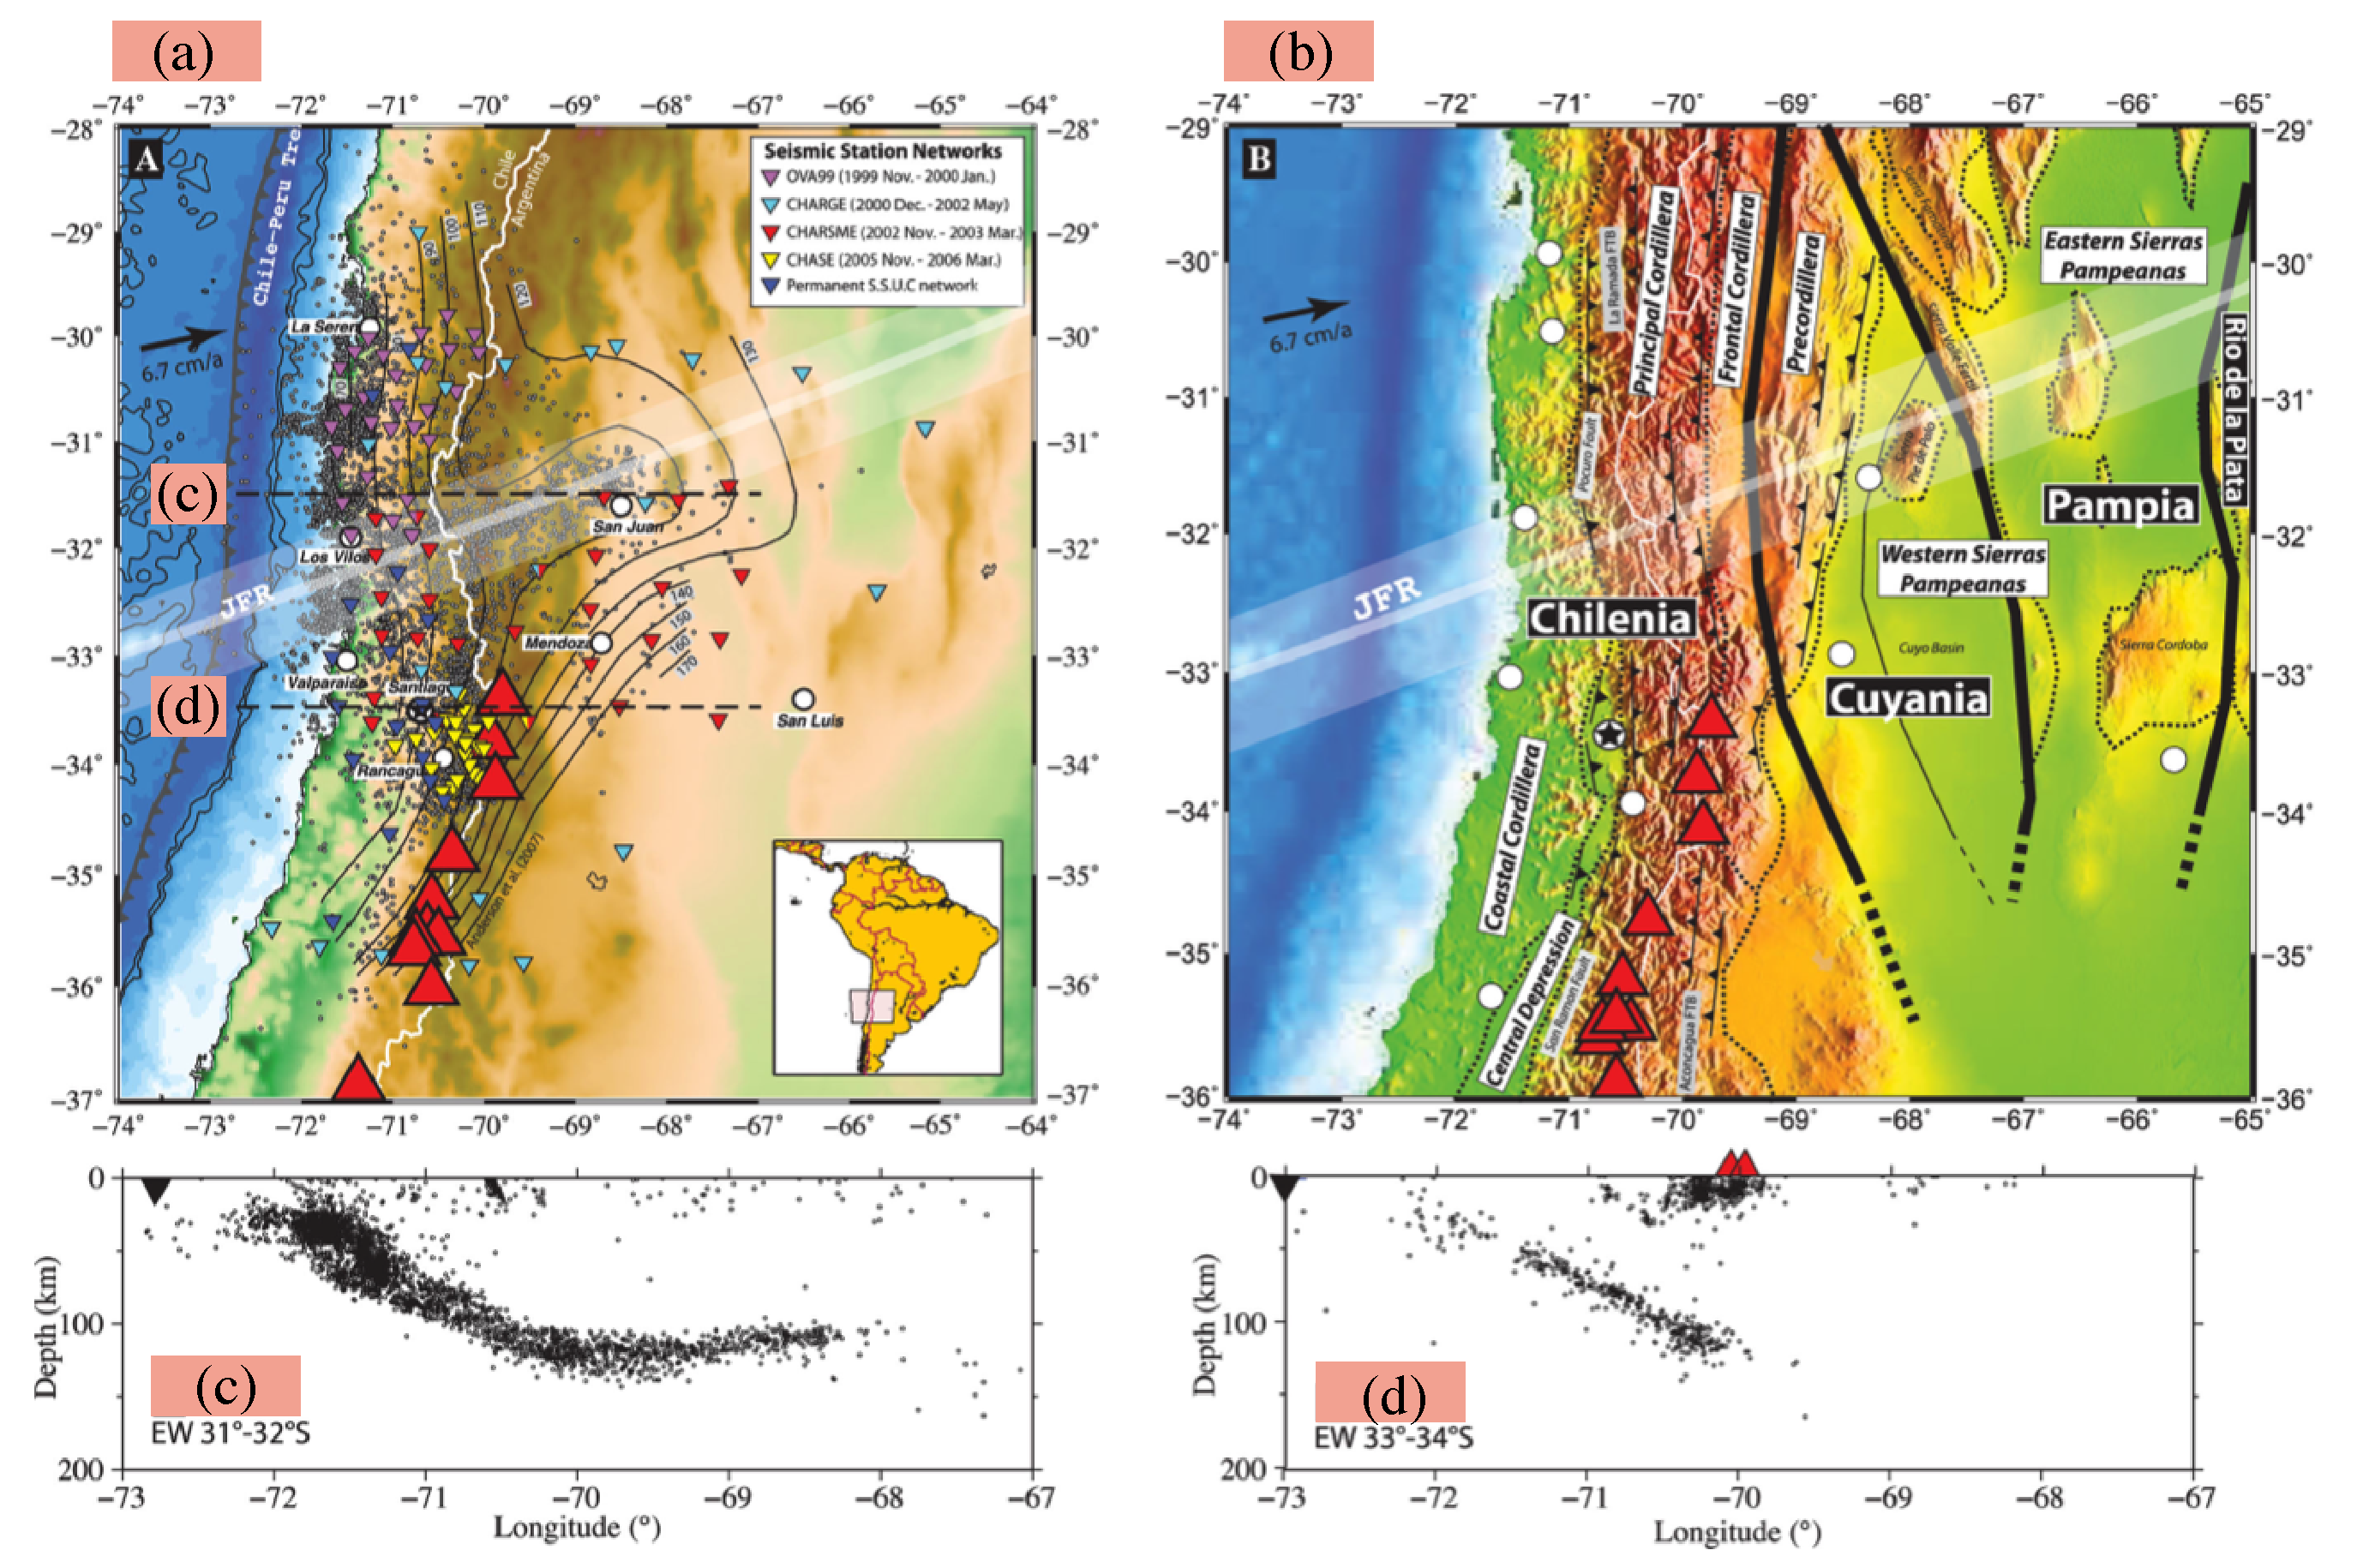
\includegraphics[width=5in]{Chile_geology_profile.pdf}
    \caption[智利中部和阿根廷西部的地質構造與地震活動度背景圖,摘自\citet{Marot2014}]{智利中部和阿根廷西部的地質構造與地震活動度背景圖,摘自\citet{Marot2014}。(a)納茲卡板塊隱沒進入南美板塊的海溝由帶三角形的黑線標出。臨時地震網以倒三角形表示,地震分佈由灰點標出,紅色正三角形為活火山分佈,隱沒板塊等深度線資料來自\citet{anderson2007geometry}。白線為智利與阿根廷的國界,白色圈圈為主要城市,其中黑色星星為智利首都聖地牙哥(Santiago)。灰線與灰透明底為推斷的胡安斐南德斯洋脊隱沒路徑與寬度,插圖為宏觀地圖,兩條黑色虛線為該研究中所觀測的剖面,分別為南緯31.5度(平坦隱沒區)與南緯33.5度(正常隱沒區)。(b)粗黑線標示主要地質縫合帶,帶三角形的黑細線為La Ramada與Aconcagua斷層,白色圈圈為主要城市,紅色正三角形為活火山分佈。(c)(d)為圖(a)中的剖面,黑色點顯示平坦板塊與正常板塊區域的地震活動,倒黑色三角形是海溝位置,紅色三角形是活火山。
    }
    \label{fig::Chile_geology_profile}
\end{figure*}

\begin{figure*}[ht!]
    \centering
    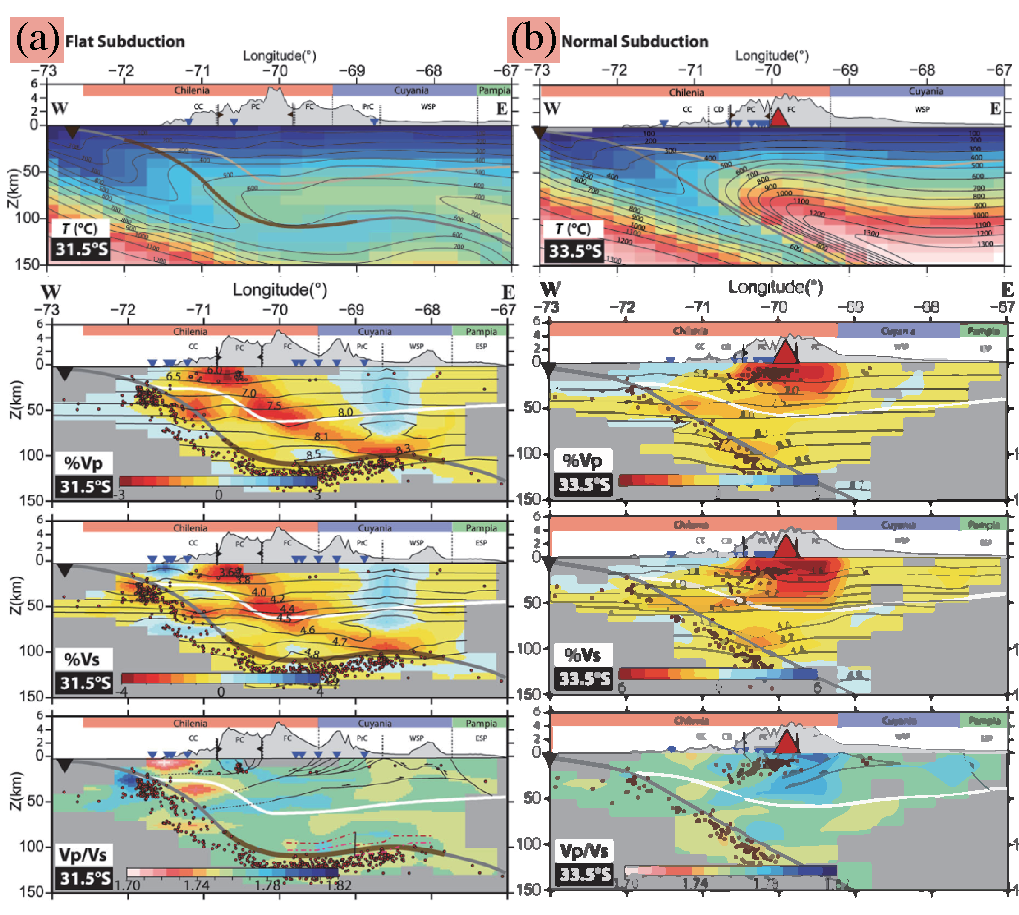
\includegraphics[width=6in]{Chile_tomography.pdf}
    \caption[智利中部和阿根廷西部的熱模型與速度構造剖面,摘自\citet{Marot2014}]{智利中部和阿根廷西部的熱模型與速度構造剖面,摘自\citet{Marot2014}。由上至下為熱構造剖面、V$_P$速度變化、V$_S$速度變化與V$_P$/V$_S$比值,速度構造剖面中的等高線為絕對地震速度。紅點代表該研究地震層析成像所選用的地震事件。白線為莫荷面,灰線為隱沒板塊頂部。(a)為圖\ref{fig::Chile_geology_profile}a中的C剖面。(b)為圖\ref{fig::Chile_geology_profile}a中的D剖面。
    }
    \label{fig::Chile_tomography}
\end{figure*}

總體而言,秘魯與智利平坦隱沒區的速度構造剖面同樣具有乾冷的地函岩石圈,且隱沒帶中平坦段的脫水作用不顯著。

\section{墨西哥隱沒帶地球物理觀測}\label{墨西哥隱沒帶地球物理觀測}
相較於南美洲,墨西哥的平坦隱沒較晚才被發現。墨西哥平坦隱沒區域位在科克斯板塊與北美板塊(North American Plate)聚合處,該地區的地震活動度較低,並且地震事件集中在距海溝100公里以內、深度20公里的範圍,因此過去難以利用地震事件隨深度分佈描繪出科克斯板塊隱沒帶的幾何形狀。

\citet{pardo1995}藉由當地地震目錄重新定位震源判斷在墨西哥中部的板塊交界處下方有平坦隱沒存在,為最早對墨西哥區域的平坦隱沒研究。
\citet{PerezCampos2008}使用接收函數方法(receiver function method)得到清晰的平坦隱沒板塊特徵,如圖\ref{fig::receiverfunction2008}。
該剖面北部顯示大陸地殼與地函之間的莫荷面,見\ref{fig::receiverfunction2008}上圖的接收函數影像,南部則些微顯示一個水平介面,如圖\ref{fig::receiverfunction2008}左下,深度落在40-50公里之間,平坦段長度約100-200公里。
有別於南美洲區域的平坦隱沒,墨西哥的平坦隱沒深度幾乎與地殼貼齊,他們起初推測長達超過100公里的板塊交界面具有強大摩擦力,理論上應有強耦合特性,亦即該地區應該容易累積大量應力產生多起地震事件。
然而正如前面所提到,墨西哥平坦隱沒段的地震活動度極低,在墨西哥平坦隱沒上方的格雷羅州擁有世界知名的格雷羅無震帶(Guerrero gap)。
GPS研究也支持該地區並不是強耦合板塊介面(\citealp{nieto2006latest})。
並且,墨西哥區域的平坦隱沒持續時間(15 Ma)比安地斯山脈平坦隱沒來得長(4-5 Ma),然而墨西哥平坦隱沒上方並沒有顯著的水平壓縮現象(\citealp{moran2007cenozoic})。
種種跡象表示墨西哥平坦隱沒區可能是弱耦合(weak coupling)的環境,與平坦隱沒的存在產生矛盾。
對此,板塊交界處需要有可行機制解釋該地區弱耦合現象。

\begin{figure*}[ht!]
    \centering
    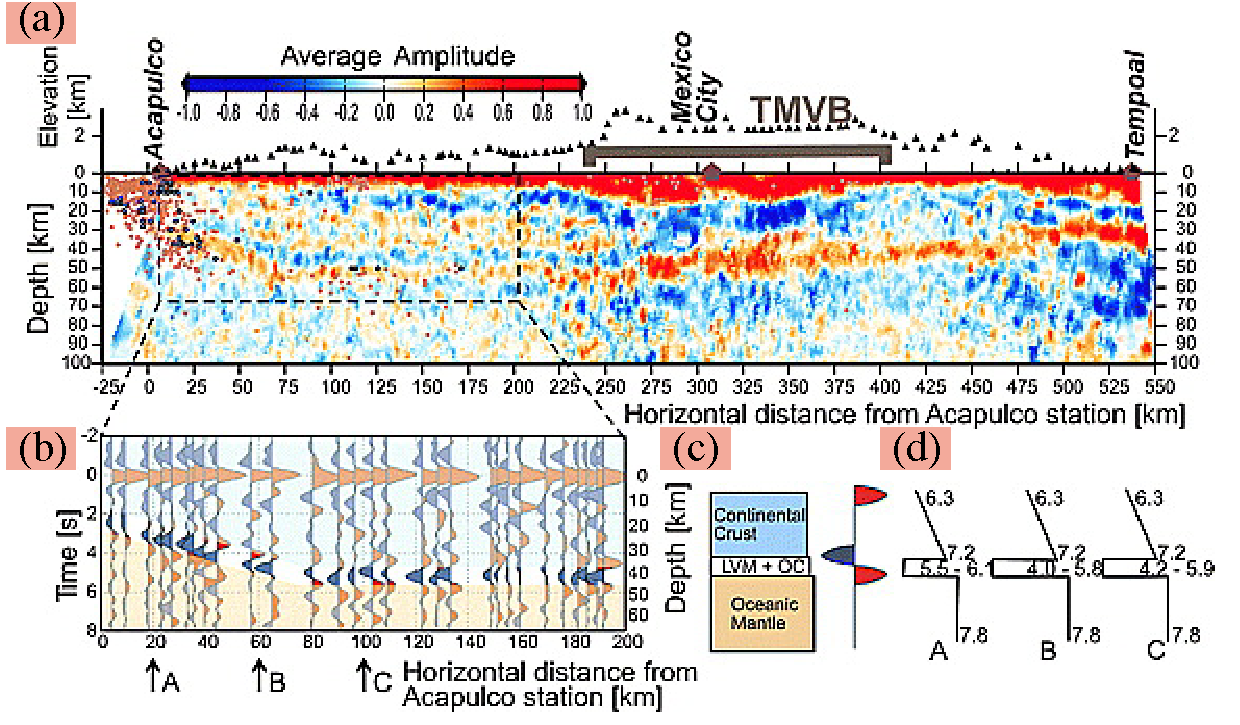
\includegraphics[width=6in]{2008receiverfunction.pdf}
    \caption[墨西哥平坦隱沒區域接收函數結果,摘自\citet{PerezCampos2008}]{墨西哥平坦隱沒區域接收函數結果,摘自\citet{PerezCampos2008}。
    (a)中黑色三角形表示測站沿剖面的位置,高程被放大10倍。
    粗棕色線表示跨墨西哥火山帶(TMVB, Trans-Mexican Volcanic Belt)的範圍。
    接收函數影像中標出沿剖面50公里範圍內的震源(粉紅色點來自SSN地震目錄,綠色點來自\citet{pardo1995}重新定位結果)位置。
    (b)顯示沿平坦隱沒板塊的一次遠震事件的接收函數。
    (c)說明了相應的模型(LVM (low velocity mantle) = 低速地函和 OC (oceanic crust) = 海洋地殼)。
    (d)根據左下圖接收函數模型中A、B和C位置上的P波速度模型。
    }
    \label{fig::receiverfunction2008}
\end{figure*}

\citet{PerezCampos2008}在平坦隱沒板塊段與大陸板塊交界處中,初步判斷有一約略10±3公里厚的低速帶,速度模型如圖\ref{fig::receiverfunction2008}右下。
他們推測該低速層很可能是弱耦合現象的主因。
\citet{Song2009}利用平坦隱沒上方地區性慢速滑移事件的轉換SP波進行波形模擬,確認該低速層厚度約3-5公里,並且其V$_S$速度約每秒2.0-2.7公里。
爾後\citet{Song2012SC}發現該低速區的地震非均向性傾角方向與隱沒板塊介面傾角方向有20±10$^{\circ}$的夾角,如圖\ref{fig::SCanisotorpy2012}所示,與S(葉理面)-C(剪切面)糜棱岩中發育的葉理方向一致,再藉由該低速區的訊號特徵,包含強烈的地震非均向性(>5$\%$)、高V$_P$/V$_S$比值、高反射率(high seismic reflextivity)與V$_S$顯著降低(-15-20$\%$),該研究推測低速層應是擁有大體積黏土礦物(例如:滑石)的變質岩,並且同時存在高孔隙流體(\citealp{Kim2012})。

\begin{figure*}[ht!]
    \centering
    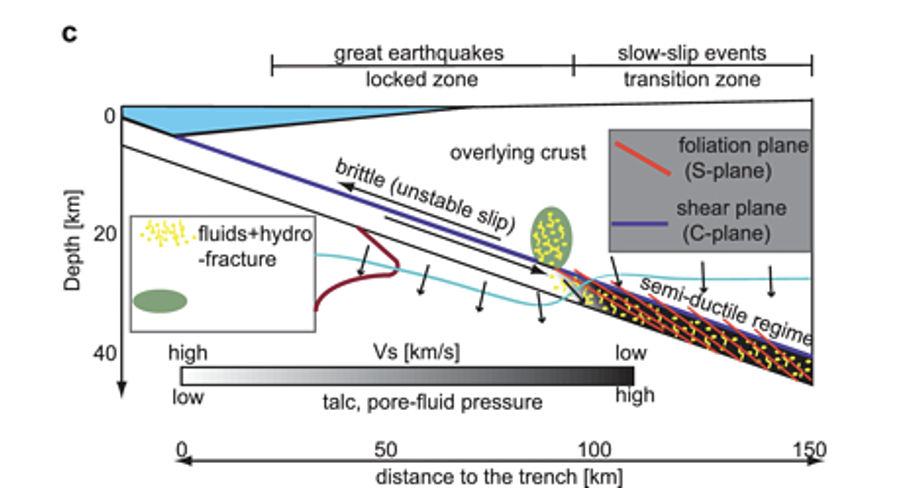
\includegraphics[width=6in]{SCanisotropy.png}
    \caption[墨西哥隱沒帶板塊介面附近剪切帶結構示意圖,摘自\citet{Song2012SC}]{墨西哥隱沒帶板塊介面附近剪切帶結構示意圖,摘自\citet{Song2012SC}。大地震主要發生在鎖定區(locked zone)和脆性(brittle)變形區域。慢速滑移事件(slow-slip event)主要發生在過渡帶(transition zone)和半韌性區域(seni-ductile regime),V$_S$非常低,且非均向性極強。這些低速帶流體導致板塊介面處於弱耦合狀態,並且主導該地區慢速滑移事件的生成。
    }
    \label{fig::SCanisotorpy2012}
\end{figure*}

%\begin{figure*}[ht!]
%    \centering
%    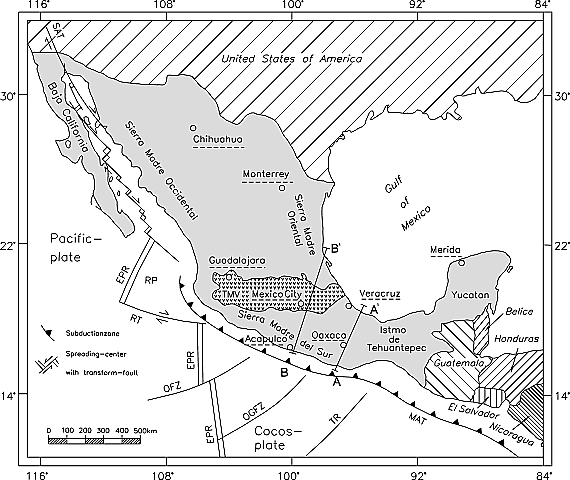
\includegraphics[width=3in]{MT_line.png}
%    \caption{\citealp{MT2006}中所使用的大地電磁剖面位置圖,本研究僅使用BB'剖面。
%    }
%    \label{fig::MT_site}
%\end{figure*}

\begin{figure*}[ht!]
    \centering
    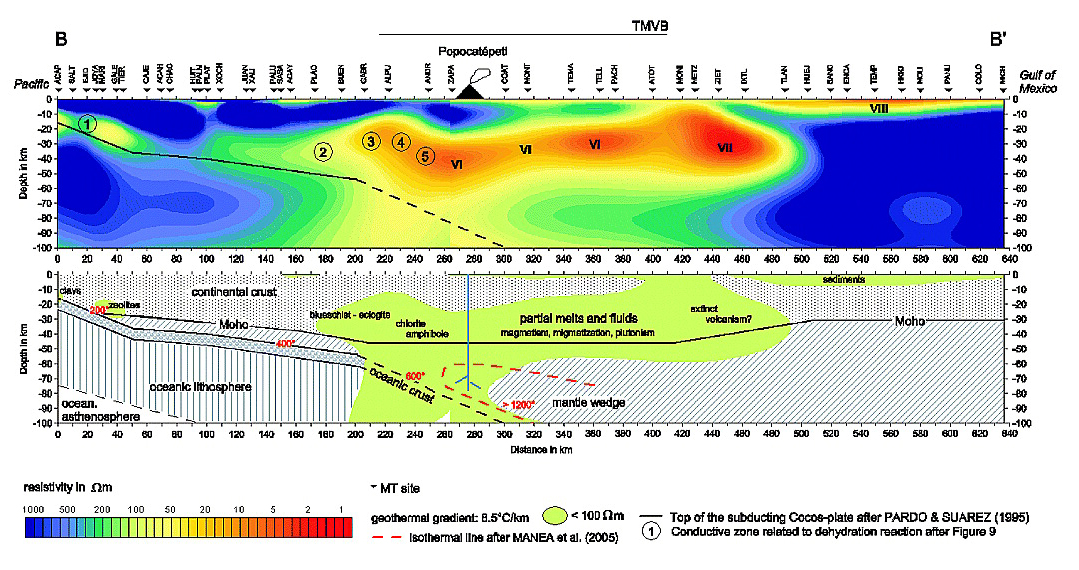
\includegraphics[width=6in]{MT_profile.png}
    \caption[墨西哥平坦隱沒區域的導電率異常剖面圖與解釋圖,摘自\citet{MT2006}]{墨西哥平坦隱沒區域的導電率異常剖面圖與解釋圖,摘自\citet{MT2006}。上圖為電阻率異常結果剖面,所繪之隱沒板塊位置參考自\citet{pardo1995}結果,最上方標示跨墨西哥火山帶的範圍。圖中每個數字圈皆代表隱沒帶上岩石發生脫水的位置,1為黏土礦物的脫水,2為藍片岩相變至綠簾石發生的脫水,3為綠簾石相變至榴輝岩的脫水,4為隱沒板塊上綠泥石的脫水,5為角閃石的脫水。下圖為電阻異常解釋圖,綠色區域為電阻異常低區(<100 $\Omega m$)。在平坦隱沒段結束處有多個岩石相變事件發生,隱沒板塊上出現大範圍導體。
    }
    \label{fig::MT_profile}
\end{figure*}

\citet{MT2006}利用大地電磁法獲得墨西哥平坦隱沒區域的導電率異常剖面(見圖\ref{fig::MT_profile}),發現在平坦隱沒結束前、隱沒板塊上方存在高導體區域,可能是隱沒板塊上物質因大量脫水產生。
圖\ref{fig::MT_profile}中編號2-5的弧前高導體區域與慢速滑移事件位置相吻合,表明該區域富含大量流體。
大量流體存在意味著脫水作用活躍,在隱沒板塊進入較高溫高壓環境下,釋放出的水分進入地函楔中,導致蛇紋岩化橄欖岩的生成。
對此,\citet{Manea2013}認為低速層可能不完全是地殼物質,而是過去因大量脫水而殘留下的地函蛇紋化橄欖岩成份,然而其內容物目前尚未完全了解。

\section{隱沒系統中的岩漿作用}\label{隱沒系統中的岩漿作用}
地球內部中,岩漿作用形成機制非常複雜,涉及部分熔融、冷卻過程結晶分異作用等。
若要使用簡單物理概念解釋部分熔融的形成,可分為三種,分別為減壓、增溫與含水,又可分別對應中洋脊(mid ocean ridge)、熱點(hot spot)與火山島弧(volcanic arc)等三種構造。
地函岩石的乾固相線通常不會與地溫梯度曲線相交,然而當發生地區性減壓作用,會導致岩石在溫度不變的情況下快速降低壓力,此時容易通過岩石固相線,發生部分熔融事件,代表構造為中洋脊。
最後,當一區域突然有額外熱源增溫,亦會導致岩石環境通過其固相線,發生部分熔融事件,代表構造為熱點火山。
聚合板塊邊界將大量地表物質帶入地球內部,物質為了在高溫高壓區維持穩定態,在隱沒過程中釋放流體,流體改變地函岩石的固相線,導致部分熔融發生,代表構造為聚合板塊邊界的火山島弧。

地函部分熔融在溫度大於攝氏850$^{\circ}$以上後容易達到固相線,岩石發生部分熔融後產生岩漿庫。
攝氏850$^{\circ}$等溫線通常距海溝水平方向上100公里左右、離地表深度80-120公里之間產生(\citealp{peacock1990fluid}; \citealp{hyndman2003serpentinization}),並會因隱沒板塊傾角大小不同而稍微有水平距離上的改變。
由此可知火山島弧的發育與隱沒板塊、地函楔的溫度狀態有強烈相關性。

平坦隱沒帶具有極端的低傾角隱沒板塊,其溫度構造與一般的隱沒帶差異甚大,因此在平坦隱沒的演化過程中,岩漿與火山作用在時間軸上會有顯著的空間變化。
平坦隱沒的低角度隱沒板塊於地函淺部趨近於水平移動,故地函楔中攝氏850$^{\circ}$等溫線會隨時間逐漸往內陸移動,亦即部分熔融發生位置會漸往內陸移動,此時上覆板塊會出現寬闊的火山帶(volcanic belt),火山帶位置從距海溝100公里延伸至400公里以上(\citealp{Gutscher2000A}; \citealp{Manea2017})。
並且,隨著平坦隱沒持續發育,溫暖的地函楔逐漸被隱沒板塊閉合,隱沒板塊上方溫度漸漸降低降低,導致火山活動度逐漸減少甚至消失(\citealp{Gutscher2000Bcan})。
除此之外,平坦隱沒帶中的熱構造因著時間軸上的演化,因此其所產生的火成岩地球化學特徵在時間軸上同樣會有顯著變化。

安地斯(Andes)山脈長約7000公里,由納茲卡板塊隱沒進入南美板塊所形成。
儘管火山島弧遍及整段安地斯山脈中,現今平坦隱沒區域上方的火山活動止於全新世早期,見圖\ref{fig::flat_slab_vol}。
秘魯區域的地球化學研究資料稀少,因此,本研究中以智利區域為主要討論範圍。
岩漿期反應了在27-20 Ma有相對較陡峭的隱沒板塊,20-9 Ma發生擠壓變形,並且在8-4 Ma之間火山島弧往內陸遷移,暗示著隱沒板塊傾角正在逐漸變淺,平坦隱沒上方的岩漿作用在5 Ma左右停止(\citealp{kay2002magmatism})。
智利區域的岩漿成分隨時間變化有SiO$_2$與K$_2$O逐漸升高的現象,且其岩漿組成變化範圍極大(\citealp{kay1988tertiary}; \citealp{kay2002magmatism}; \citealp{goss2013andean})。

在智利平坦隱沒區域最北段的火成岩地球化學特徵被歸類為埃達克岩(adakite),約略出現於8-3 Ma之間,如圖\ref{fig::Chile_adakite_map}b中黃色圈處。
\citet{Gutscher2000Bcan}嘗試提出一地溫梯度極高的大陸岩石圈模型,導致隱沒板塊發生平坦隱沒後,板塊頂部溫度達到攝氏700-800$^{\circ}$,此時隱沒板塊上的部分熔融便可輕易發生。
儘管\citet{Gutscher2000Bcan}解釋認為智利的埃達克岩是隱沒板塊熔融所造成,並且是平坦隱沒中的一個重要過程。
然而\citet{kay2002magmatism}、\citet{goss2013andean}卻認為平坦隱沒帶中的上覆板塊溫度無法達到如此高溫,因而提出埃達克岩的來源應為大陸地殼熔融,而非海洋地殼熔融的概念模型。
他們的證據建立在智利埃達克岩的同位素特徵,該結果顯示其內容物由高壓大陸地殼岩石成分(石榴子石, garnet)所主導(\citealp{kay2002magmatism})。
目前對於智利區域埃達克岩的成因還有很大的討論空間,本研究將會在\ref{平坦隱沒中的埃達克岩}章節中進行更詳細的討論。

墨西哥境內的跨墨西哥火山帶(Trans Mexico Volcanic Belt)橫跨東西向墨西哥,約在25 Ma前後生成,該時期與可能的平坦隱沒初始發育期有關。
跨墨西哥火山帶在中新世早期至中期(Early to Late Miocene, 19-8 Ma)的侵入岩以安山岩為主,可見圖\ref{fig::Mexico_adakite_map}墨西哥的火成岩分佈地圖。該時期火山島弧寬度從西向東有顯著側向變化,東北邊的岩漿作用逐漸遠離海溝,火山帶隨時間拉寬,導致火山島弧分佈與海溝呈現非平行的狀態,並且岩漿活動逐漸減小甚至消失。
地球化學分析認為該段時期的火成岩有隱沒流體量隨時間逐漸減少的特徵,並且安山岩的矽質成分逐漸變高,演變成英安岩(dacite)。
這個趨勢在15 Ma左右被侵入的埃達克岩中斷(\citealp{mori2007effects}),這些埃達克岩樣本被認為是隱沒板塊熔融的產物(\citealp{gomez2003temporal}; \citealp{mori2007effects}),埃達克岩會在\ref{平坦隱沒中的埃達克岩}章節中有詳細的討論。
總結來說,這段時間諸多地球化學特徵暗示著平坦隱沒正在發育,包含火成岩成分從玄武岩質安山岩(basaltic andesitic)逐漸變成英安岩、岩漿特徵隨時間演進有越來越多地殼的貢獻、岩漿作用與海溝的距離隨時間增加以及許多埃達克岩特徵的樣本出現。
平坦隱沒的發育止於11 Ma,此時火山島弧前緣(volcanic front)距海溝約450公里(\citealp{Manea2011Thermal})。
自11 Ma起火山島弧前緣開始以每百萬年10公里的速度往海溝移動,同時,鐵鎂質岩漿的成分開始變多,可能是平坦隱沒開始回捲(rollback)過程中,地函楔橄欖岩的減壓熔融產物(\citealp{gomez2003temporal})。
如今的火山島弧前緣約略與海溝距離350公里,有穩定活躍的火山活動現象。

\begin{figure*}[htp]
    \centering
    \includegraphics[width=6in]{Chile_adakite_map.pdf}
    \caption[智利火山分佈,摘自\citet{goss2009extreme}]{智利火山分佈,摘自\citet{goss2009extreme}。
    (a)南美洲西海岸和安第斯山脈主要構造形態特徵示意圖,改編自\citet{lamb2003cenozoic}。虛線為國界。黑色箭頭表示\citet{demets1990current}的平均聚合速度。板塊等深度線為灰色粗線,海拔高度2000公尺以上區域以橘色表示。三角形標示出活火山位置,NVZ = 北部火山區,CVZ = 中部火山區,SVZ = 南部火山區。黃色陰影框表示北部平坦隱沒區與過度區(27.5°–28.5°S)。
    (b)顯示圖(a)中黃色陰影框地圖。黑色實線為現代中部火山島弧位置,黑色短虛線為中新世火山島弧弧前位置。中生代火山島弧寬度由黑細線標出範圍。中生代火山島弧的侏羅紀 La Negra 玄武岩和輝長岩的露頭以灰色陰影顯示,新近紀玄武質火山活動地點由白星表示。黑色箭頭顯示約 50 公里的晚中新世火山島弧向東遷移。埃達克質火山活動區域由黃色圈圈表示,包括約 8 Ma Dos Hermanos lava、7-6 Ma與6-3 Ma的Pircas Negras和 3-2 Ma 的 Rio Salado Pircas Negras。
    }
    \label{fig::Chile_adakite_map}
\end{figure*}

\begin{figure*}[ht!]
    \centering
    \includegraphics[width=6in]{Mexico_map_adakite.pdf}
    \caption[中新世早期至晚期跨墨西哥火山帶火成岩分佈,摘自\citet{ferrari2012dynamic}]{中新世早期至晚期跨墨西哥火山帶火成岩分佈,摘自\citet{ferrari2012dynamic}。其中,黃色圈起處的火山為具有埃達克岩組成的火山。圓點表示\ref{平坦隱沒中的埃達克岩}節中圖\ref{fig::Cocos_geochemisty}進行地球化學分析的樣本位置,星星表示進行定年分析的樣本位置。紅圈圈處的Chalcalzingo domes為20 Ma前後出現的流紋岩樣本,具有非常高矽質埃達克岩成份,被視為該區最早的火成岩樣本,並且其成份為幾乎無雜質的隱沒板塊熔融物質(\citealp{gomez2008origin})。
    }
    \label{fig::Mexico_adakite_map}
\end{figure*}
% !TeX root = ../main.tex

\chapter{數值模型}

同第一章所述,地球動力學為探討地球內部的動力過程,以及地球內部物質受力後所發生的變形作用,其所牽扯的運動過程複雜。
地質學藉由地表觀察,可得知過去地表上經歷的地質事件,進而間接獲得當時的動力狀態,不過隨著時間推移,可用的岩石紀錄越來越少,並且地質資料並無法完全代表地球內部的動力過程。
地球內部的直接觀察僅能靠鑽井資料獲取,然而地球上最深的鑽井資料為12公里(\citealp{ganchin1998seismic}),不到地球半徑的千分之二。
因此,只能靠間接方法探測地球內部,地球物理學便是強大研究學門。
地球物理學包含多種研究,重力學、磁力學、大地電磁等方法利用矩陣逆推(inversion)計算地表測站資料,獲得地下構造成像,不過這些方法並不是接收直接通過地球內部介質而來的訊號,因此約束不多且深度解析有限。
地震波能量穿透整個地球被全球地表測站接收,過程中地震波直接通過地球內部介質,為地球內部構造提供有效的資訊,故地震學為目前最常見對地球深部構造的探勘方法。
儘管如此,最早的地震學發展始於19世紀末,其所觀測得之構造在地質時間尺度上只能被視為瞬間狀態,無法代表地球內部過去的構造狀態。
為了彌補地球內部在時間上與空間上的有限數據量,地質建模與模擬成為探討地球內部演化的有力工具。

在本研究的數值模型中,地球動力學所牽扯的運動過程複雜,不適用單純的質點或剛體運動,需要使用連續體力學(Continuum mechanics)的物理概念描述岩石的動力與變形行為。
在模型中將岩石單元視為地質構造上的連續介質(Continuum media),岩石具有巨觀物理量,受牛頓力學所支配,系統中的總力除了質點運動中所包含的外力(external force)之外,還需要考慮系統的內部作用力(internal force)。
連續介質特性描述可被用於岩石的密度、壓力、速度、應變等不同維度物理的場變量(field variables)。
由於在地質尺度上長期且緩慢的岩石變形過程可視為流體,因此地球動力學模型在不同尺度上部分可視為流體力學的展現。
而流體力學的數學式共有三大守恆定律,分別為質量守恆、動量守恆與能量守恆。
該三大守恆定律可寫成偏微分方程式的形式,同時也是連續方程式,此時因偏微分方程式之解析解多半不存在,僅能利用數值近似方法求得最佳解。

在本章節中會介紹數值模擬的計算方式以及模型物質物理特性。

\section{FLAC}

本研究使用Fast Lagrangian Analysis of Continua (FLAC,快速拉格朗日連續體分析) 技術,最早是由\citet{cundall1989numerical}開發的二維顯性(explicit)有限差分(Finite Difference Method, FDM)數值分析程式。
爾後由\citet{Lavier2000}改良,適用於模擬地球動力與地球內部變形。
FLAC使用拉格朗日描述法(Lagrangian formulation)與非均值網格(structured non-uniform mesh),在符合牛頓力學的情況下,於每個時間段上求解每個節點(node)的運動方程式,算出每個節點上所受到的力,計算出新的速度與位移,獲得節點應變,再藉由岩石流變學物性方程式(constitutive equation)從應變推得節點所受應力,作為下一時間的初始作用力,流程見圖\ref{fig::FLAC_method}。

\begin{figure*}[ht!]
    \centering
    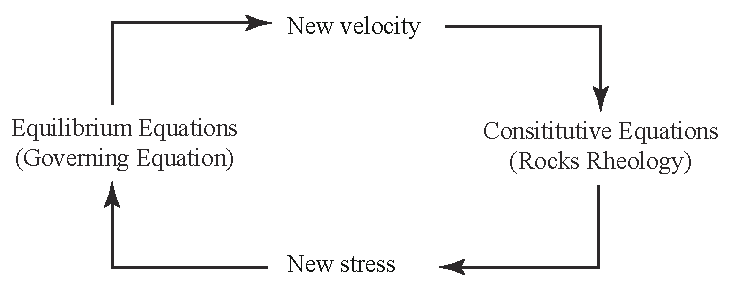
\includegraphics[width=4in]{FLAC_flow.pdf}
    \caption[FLAC 程式運算流程圖]{FLAC 程式運算流程圖。}
    \label{fig::FLAC_method}
\end{figure*}
單一網格中存在一定數量的標記點(marker),紀錄岩相、位置等特徵,標記點的速度由計算獲得的速度決定,可在網格間移動。
由於模型中的網格會根據所受的應力變形,在一段時間內若網格扭曲嚴重、網格的邊界角度過大或過小,則FLAC會重建網格,該過程稱為網格重建(remesh)。
此時所有網格與節點會重新排列,並使用差分標記點上的物理量獲得新節點的物理量。

FLAC所使用的主控方程式包含質量守恆、動量守恆與能量守恆方程式。考量岩石流變學中的彈性、塑性與黏性變形行為,以下將一一介紹主控方程式與岩石流變學。
\section{主控方程式}

\subsection{質量守恆}
由於FLAC使用拉格朗日描述法,每個拉格朗日點被嚴格的連到一單一的物質點上,並且會隨著該點移動。
因此,同一個質點總是在同一座標上,與時間無關,該座標滿足質量守恆。
拉格朗日描述法的質量守恆方程式如下:
\begin{align}
\frac{D\rho}{Dt}+\rho\nabla\cdot\vec v =0 
\label{eqn:MASS_Lagrangian}
\end{align}
其中 $\frac{D\rho}{Dt}$ 表示拉格朗日座標下的密度隨時間變化,$\rho$為密度,$\vec v$為速度向量。

\subsection{動量守恆}
地球內部的動力包含了介質所受之外力與內力力平衡的結果,並且在物質受力後產生變形。
在數值計算中利用動量守恆方程式將力與變形聯繫,滿足牛頓第二運動定律。
\begin{align}
\vec f=m\vec a
\end{align}
$f$ 為作用在物質上的作用力,$m$為物質的質量。
本研究所使用之拉格朗日坐標系下動量守恆方程式為:
\begin{align}
\rho \frac{ Dv_{i}}{Dt} = \frac{\partial \sigma_{ij}}{\partial x_j}+\rho g_i\label{eqn:momentum Lagrangian}
\end{align}
或
\begin{align}
\rho \vec a = \nabla\cdot\vec\sigma+\rho\vec g\label{eqn:momentum Lagrangian2}
\end{align}
此為Navier-Stokes方程式。 其中$\rho$為密度,$\vec a$為節點加速度,$\vec\sigma$為應力張量(stress tensor),$g$為重力加速度。

\subsection{能量守恆}
為了描述一連續體中的能量平衡狀態,使用溫度方程式表示能量的進出。
拉格朗日描述法下的能量守恆方程式表示如下:
%\begin{align}
%\rho C_p \frac{DT}{Dt} = -\frac{\partial q_x}{\partial x}-\frac{\partial q_y}{\partial y}-\frac{\partial q_z}{\partial z}+H_s+H_L
%\end{align}
%將熱通量拆解:
%\begin{align}
%q=-k\frac{\partial T}{\partial x}
%\end{align}
\begin{align}
\rho C_p \frac{DT}{Dt} = k\nabla^2T+H_s+H_L
\label{eq:heat equation}
\end{align}
式\ref{eq:heat equation}為拉格朗日座標下標準的熱擴散方程式加上額外的兩種熱源,分別為摩擦熱($H_s$, friction heat)與潛熱($H_L$, latent)。
其中$T$是溫度,$\rho$是密度,$C_p$是等壓比熱容量,$k$是熱傳導係數。
摩擦熱($H_s$)由剪切力在不可逆變形中能量耗散所產生,通式如下:
\begin{align}
    H_s = \sigma^{'}_{ij}\dot\varepsilon^{'}_{ij}
\end{align}
$\sigma^{'}$為軸差應力(deviatoric stress),$\dot\varepsilon^{'}$為軸差應變率(deviatoric strain rate)。

潛熱($H_L$)為物質發生相態變化過程中,溫度不變時釋放或吸收的能量,本研究唯一有考慮的潛熱為岩漿結晶中產生的放熱,在\ref{岩漿作用造成的溫度影響}節中有較詳細的介紹。
本研究中並沒有考慮放射性元素所產生的熱。
主控方程式沒有考慮絕熱(adiabatic)溫度梯度,因此動力過程中的溫度皆不包含絕熱溫度,然而本研究在不影響動力過程的相變與岩漿作用下有考慮絕熱溫度梯度。

\section{岩石流變學}
主控方程式包含七個方程式與十個未知數,因此求解過程需要額外方程式。
岩石的流變學由物性方程式所表示,不同的岩石具有不同物理性質。

在近地表區域,岩石處於相對較低溫的環境,因此地球岩石圈表層由脆性變形(brittle deformation)所主導,包含低壓下的彈性變形(elastic deformation)與高壓下的塑性變形(plastic deformation)。
而在地球岩石圈深處到地球內部,岩石因周遭溫度隨深度增加而表現出不可逆的黏性變形(viscous deformation)。
因此,若地球動力學模型需同時考慮廣泛的岩石變形特性時,則模型流變學應同時包含彈-塑-黏性(elasto-visco-plastic)變形。

彈性變形假設物質所承受的應力與其應變呈正比,可以是虎克定律的展現。彈性變形很重要的精隨為其變形是可逆的,若施加在彈性物質上的應力被移除,其變形量會變回零。
由虎克定律得到彈性通式:
\begin{align}
\sigma_{ij}=E_{ijkl} \varepsilon_{kl}
\end{align}
其中,$\sigma$為二階應力張量(stress tensor),$E$為四階張量彈性常數(elastic constant),$\varepsilon$為應變。
假設物質具有均質性(isotropic),則上列通式矩陣僅會有兩個獨立分量:

\begin{align}
    \sigma_{ij}=\lambda_1 \varepsilon_{kk} \delta_{ij}+2 \lambda_2 \varepsilon_{ij}=K\varepsilon_{kk} \delta_{ij}+2 \mu \varepsilon_{ij}^{'} \label{eqn:elastic tensor}
\end{align}
這裡的$\sigma_{ij}$為本研究所使用的彈性應力$\sigma_{elastic}$。

彈性力學所使用的拉梅參數為$\lambda_1 = \lambda_2 = 3 \times 10^{10} Pa$,$\varepsilon^{'}$為軸差應變,其中第一拉梅參數(Lamé's first parameter, $\lambda_1$)與體彈性系數(bulk modulus, $K$)、剪彈性系數(shear modulus, $\mu$)的關係式如下:
\begin{align}
\lambda_1 = K - \frac{2}{3}\mu
\end{align}

第二拉梅參數(Lamé's second parameter, $\lambda_2$)等同於剪彈性系數。

本研究所使用的塑性變形滿足莫爾庫倫破壞準則(Mohr-Coulomb)定義屈服應力(yield stress)大小:
\begin{align}
    \sigma_{yield}=C+tan(\phi)\sigma_{n}\label{eqn:plastic deformation}
\end{align}
這裡的屈服應力(yield stress)等同本研究中的塑性應力$\sigma_{plastic}$。
其中$C$為內聚力,$\sigma_n$為正向力,$\phi$為物質摩擦角。
當物質不可逆變形(破壞)發生後,達到再次破壞變形所需的應力會大幅下降,這是物質應力弱化(strain weakening)的展現,其內部內聚力與摩擦角皆會降低,伴隨著物質強度降低。
本研究中假設已破壞物質之內聚力與摩擦角會線性降低直到一飽和最小值,如圖\ref{fig::plastic_deformatiom},表示發生過破裂的物質強度變弱。
岩石摩擦角與內聚力的值會隨應變率從0到$\varepsilon_{pl,saturate}$之間在($C_0$, $\phi_0$)與($C_1$, $\phi_1$)之間線性遞減,隨後達到摩擦角與內聚力的飽和最小值。
本研究各物質所使用的內聚力與摩擦角見表\ref{table::phase_table}。
\begin{figure*}[ht!]
    \centering
    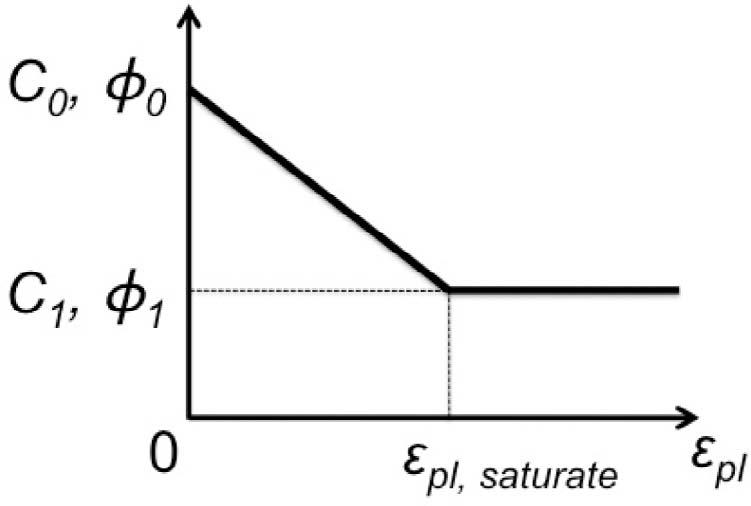
\includegraphics[width=3in]{Tan 2012 plastic.jpg}
    \caption[應力弱化示意圖,摘自\citet{Tan2012}]{應力弱化示意圖,摘自\citet{Tan2012}。在應變率為$0$時,岩石摩擦角與內聚力分別為$C_0$, $\phi_0$; 在應變率大於$\varepsilon_{pl,saturate}$時,岩石摩擦角與內聚力分別為$C_1$, $\phi_1$。摩擦角與內聚力的值會隨應變率變化在($C_0$, $\phi_0$)與($C_1$, $\phi_1$)之間線性遞減。
    }
    \label{fig::plastic_deformatiom}
\end{figure*}

最終採用的彈塑性應力$\sigma_{elasto-plastic}$依照彈性應力($\sigma_{elastic}$)與塑性應力($\sigma_{plastic}$)的量值決定,共可分為兩種情形:

1. 若$\sigma_{elastic} <= \sigma_{plastic}$,則$ \sigma_{elasto-plastic} = \sigma_{elastic}$,物質不發生破壞。

2. 若$\sigma_{elastic} > \sigma_{plastic}$, 則物質發生破壞,需將$\sigma_{elastic}$投影至屈服面上以獲得物質發生破壞最小所需應力$\sigma_{elasto-plastic}$ (\citealp{simo2006computational})。

當溫度較高,材料強度相對進地表較低,以黏彈性(visco-elastic)變形為主。
本研究使用實驗結果所得的非牛頓流體位錯蠕變定律(dislocation creep laws)定義岩石黏滯度(\citealp{Chen1990}):
\begin{align}
   \eta=\frac{1}{4}(\frac{4}{3A})^{\frac{1}{n}} \dot\varepsilon_{II}^{' \frac{1-n}{n}} exp(\frac{E}{nR(T+273)})
   \label{eqn:viscousity}
\end{align}
$\eta$為黏滯度,$\dot\varepsilon^{'}$為軸差應變率張量矩陣,$\dot\varepsilon_{II}^{'}$為軸差應變率張量矩陣的第二不變量,$n$為應力冪數(stress exponent),$A$為材料的指數前因子(viscosity pre-exponent),$T$為攝氏溫度,$E$為活化能(activation energy),$R$為氣體常數(universal gas constant),本研究各物質所使用的應力冪數、材料的指數前因子與活化能見表\ref{table::phase_table}。
由於黏滯度會隨溫度升高而降低,本研究中,施加一臨界黏滯度最小值至10$^{20}$ Pa$\cdot$s,以防止黏滯度過低導致計算量過大。
黏彈性應力與黏滯度、應變率成正比,其計算方式如下:
\begin{align}
    \sigma_{viscous} = 2\eta\dot\varepsilon^{'} \label{eqn:viscous tensor}
\end{align}
最終採用的黏彈性應力$\sigma_{elasto-viscous}$為馬克士威模型(Maxwell model),其為一純黏性阻尼與純彈性彈簧串連組成。

在同一網格中會分別計算每個網格上的$\sigma_{elasto-plastic}$與$\sigma_{elasto-viscous}$,每個網格所採計的應力值為($\sigma_{elasto-plastic}$, $\sigma_{elasto-viscous}$)兩者之間的最小值。
模型的岩石強度剖面示意圖如圖$\ref{fig::strength}$所示。
\begin{figure*}[ht!]
    \centering
    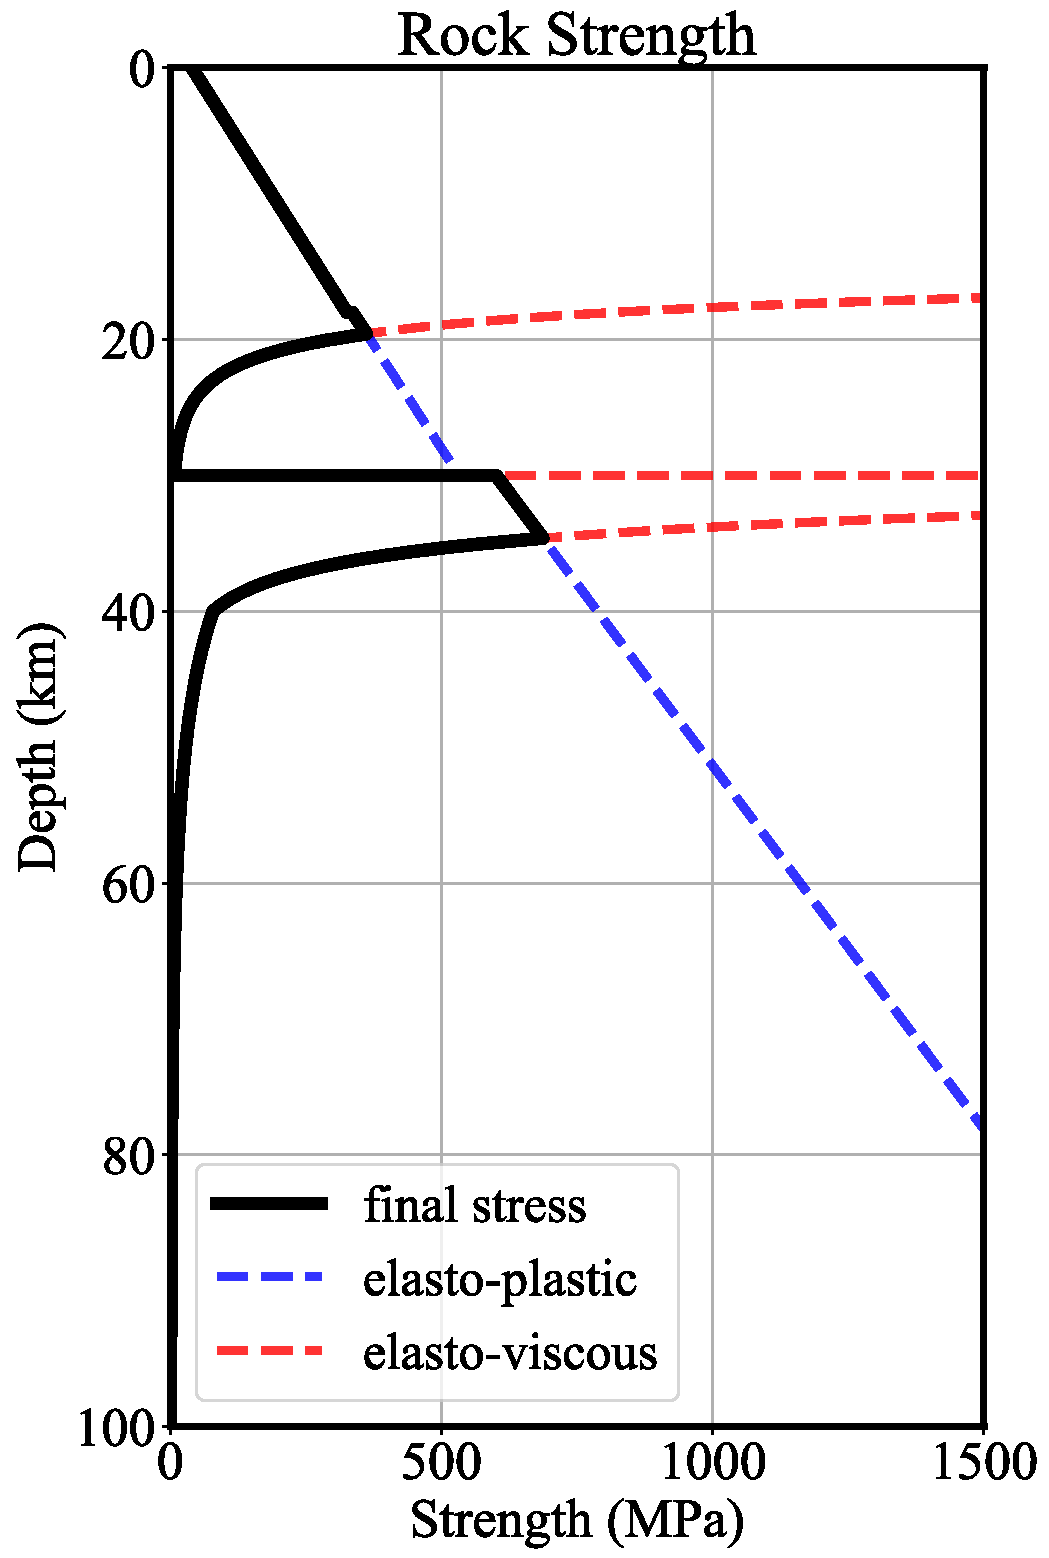
\includegraphics[height=3in]{strength_v3.pdf}
    \caption[岩石強度剖面示意圖]{岩石強度剖面示意圖,藍色虛線為彈塑性變形; 紅色虛線則為黏彈性變形。黑色實線為最終強度,採用$\sigma_{elasto-plastic}$, $\sigma_{elasto-viscous}$兩者之間最小值。}
    \label{fig::strength}
\end{figure*}

\section{相變}\label{相變}

為了模擬自然界中岩石動力學中的物理性質變化,本研究考慮部分岩石相變機制,利用岩石溫度壓力狀態當作簡單相變條件。
考量相變過程可以讓隱沒模型之運動況狀以更真實的型態呈現,更能真實展現隱沒帶中力學分配過程。

在本研究中,使用模型中的標記點追蹤物質之岩相與位置,一旦所在網格之溫度與壓力滿足標記點物質之相變條件,則會判定該標記點發生相變,其岩相轉換為相變後之新岩相。
相變完成後,標記點物質所有物理性質皆會從原先岩相之性質轉變成新岩相之性質。
由於相變過程不影響運動狀態,但與溫度相關,因此模型中在考慮相變時,該位置溫度會將絕熱溫度梯度加回模型的溫度中。
以下將一一列出模型中所考慮的相變過程。

\subsection{蛇紋岩化的橄欖岩}\label{蛇紋岩化的橄欖岩}
一旦隱沒板塊進入地函中,隱沒海洋板塊上之沉積物在高溫高壓下會釋放大量流體至楔中,絕大部分集中在地函楔。乾的地函楔因而經歷水合作用,導致部分橄欖岩被蛇紋岩化。
蛇紋岩化橄欖岩(serpentinized peridotite)在這裡又稱為蛇紋岩(serpentinite),主要集中於隱沒帶中淺部,並且目前人類對於蛇紋岩之相變作用尚未有高度不確定性,因此本研究中以參數化方式模擬蛇紋岩相變過程。
使用者可自行調整在隱沒板塊上方有多少厚度的地函楔會因脫水作用相變成蛇紋岩(\citealp{Tan2012}),見圖\ref{fig::serpeninite_parameter}。
在本研究中,蛇紋岩之岩相物理性質約略等同於橄欖岩中有百分之15之橄欖岩被蛇紋岩化,過去的實驗指出其相比於橄欖岩,活化能大幅減少(\citealp{hilairet2007high}),因此蛇紋岩強度極弱,遠小於普通地函。

\begin{figure*}[ht!]
    \centering
    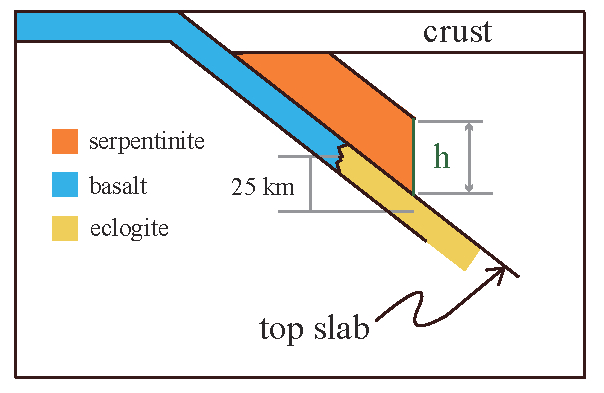
\includegraphics[width=4in]{serpeninite_parameter.pdf}
    \caption[蛇紋岩參數化示意圖]{蛇紋岩參數化示意圖。於模型隱沒板塊上,海洋地殼玄武岩相變成榴輝岩深度後25公里深之上的地函會生成h公里厚的蛇紋岩。}
    \label{fig::serpeninite_parameter}
\end{figure*}

蛇紋岩將隱沒帶流體帶入更深的地函中後,約在80-120公里之間再次發生脫水將水分釋放至地函楔中。
本研究中,在符合以下溫壓條件時(\citealp{Ulmer1995}),該脫水作用成立,蛇紋岩將相變回橄欖岩:
\begin{align}
P > 2.1 + (7.5-2.1)\times (T-730)/(500-730) \quad GPa \\
P > 2.1 + (0.2-2.1) \times (T-730)/(650-730) \quad GPa
\end{align}
其中$T$為攝氏($^\circ C$)。
圖\ref{fig::serpentinite_phase_diagram}為橄欖岩相溫壓相圖。
\begin{figure*}[h!]
    \centering
    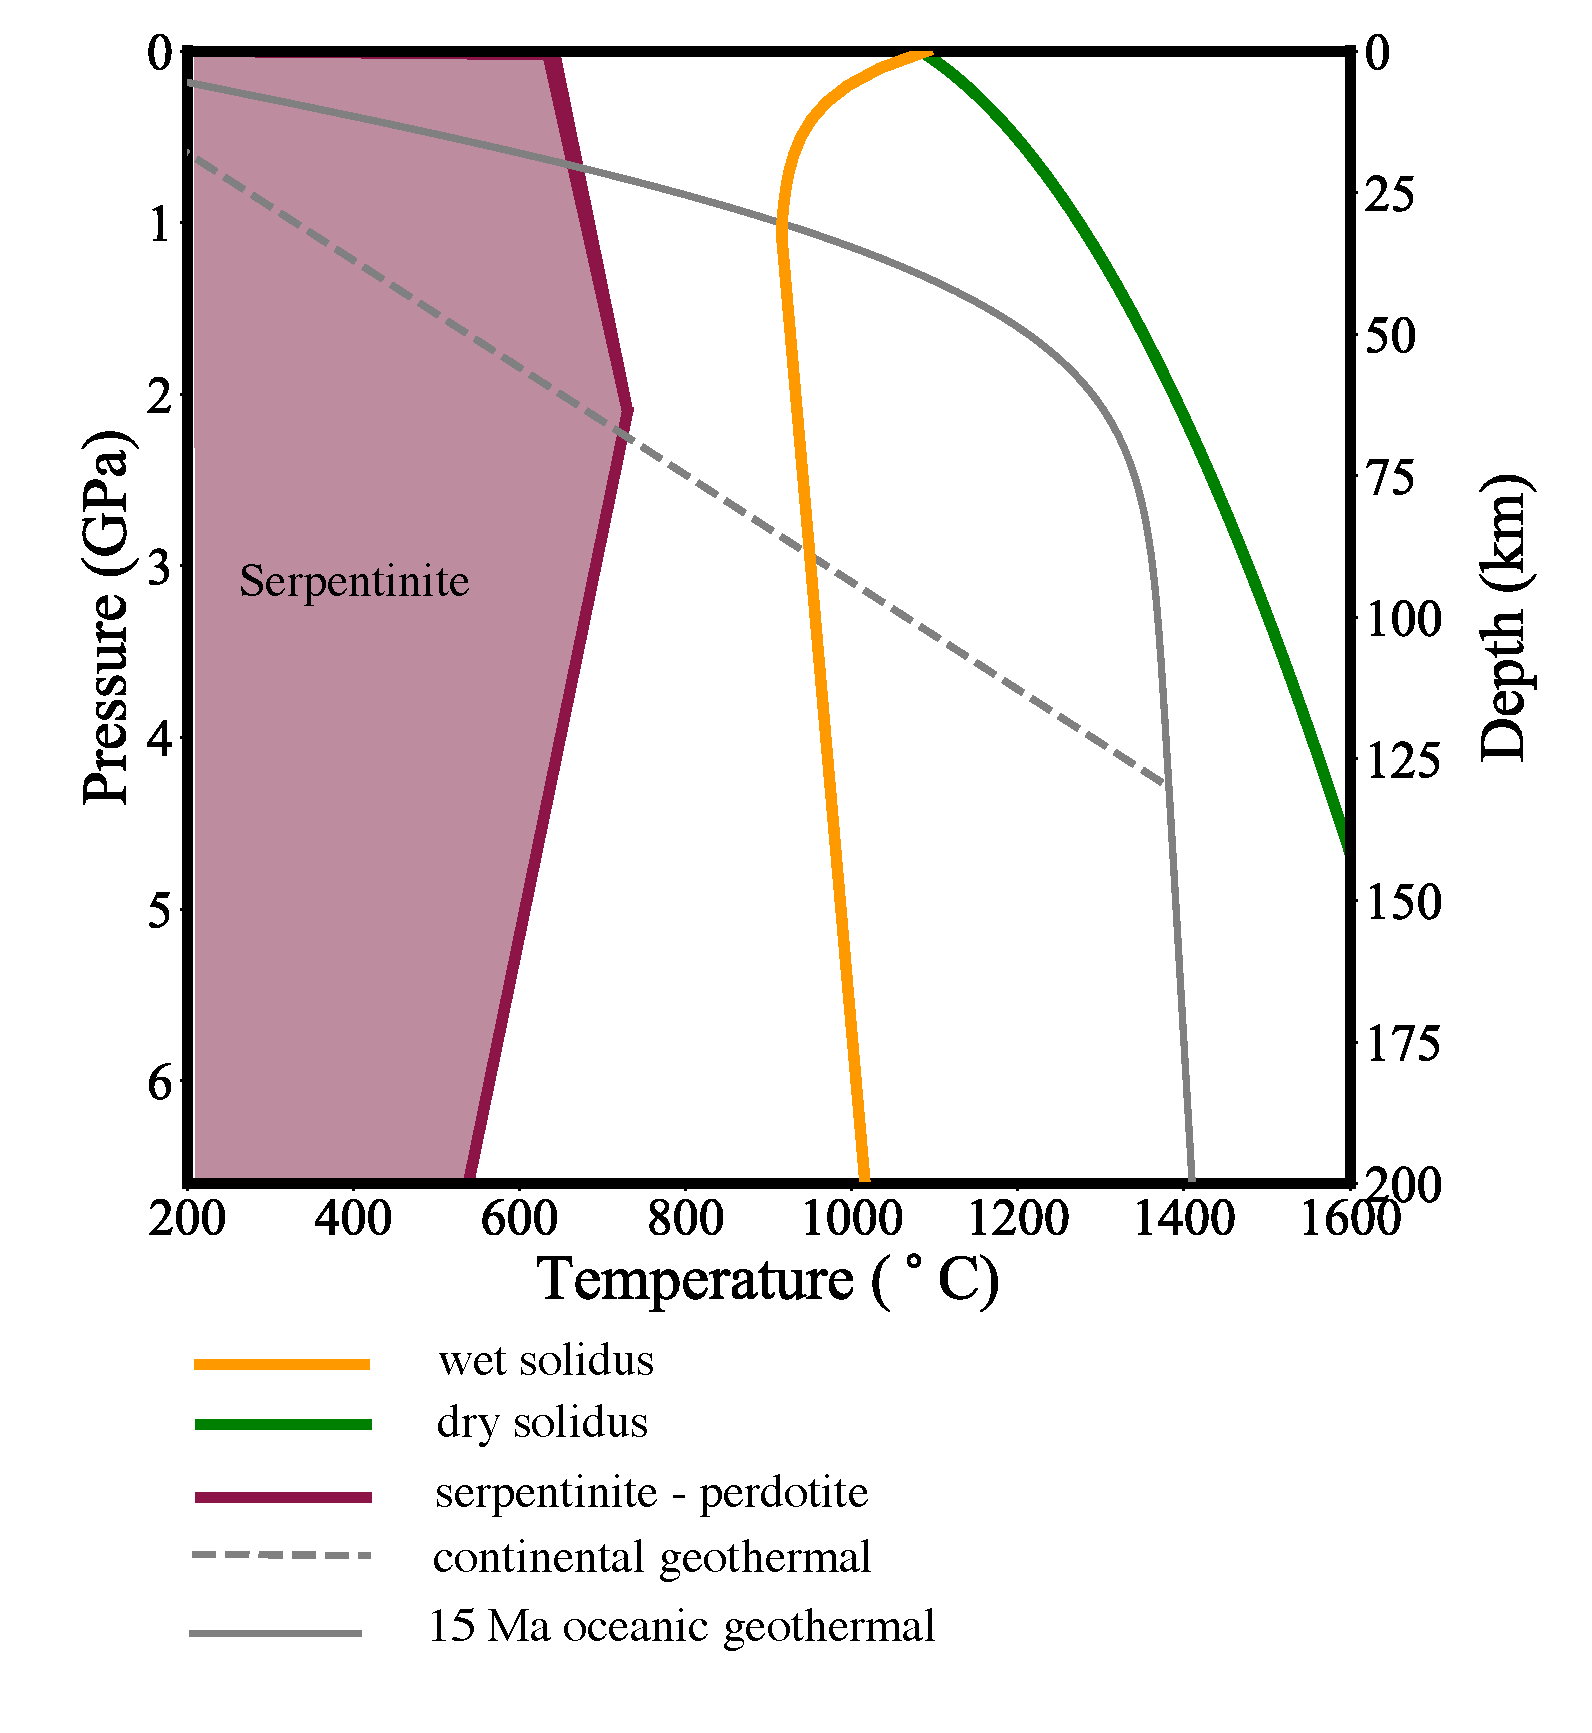
\includegraphics[width=4in]{serpentinite_phase_diagram_v1.pdf}
    \caption[橄欖岩相圖,參考\citet{Ulmer1995}]{橄欖岩相圖。紫線代表蛇紋岩脫水回橄欖岩之相變圖,參考\citet{Ulmer1995}。綠線與黃線分別代表橄欖岩的乾固相線(dry solidus)與含水固相線(wet solidus),摘自\citet{katz2003new}。另用灰線實線與虛線分別表示墨西哥參考模型之海洋岩石圈與大陸岩石圈地溫梯度。}
    \label{fig::serpentinite_phase_diagram}
\end{figure*}

本研究所使用的橄欖岩含水固相線(wet solidus)參考自\citet{katz2003new},簡化式如下。
\begin{align}
    T > max (980+6\times (3.3 \times P-14) ,\quad 1090-178\times(1-exp(-4.125\times P))) ^\circ C 
\end{align}
其中$P$為十億帕斯卡(GPa)。

\subsection{玄武岩 --- 榴輝岩}

隨著隱沒板塊沉入更深的地函,其上的鎂鐵質玄武岩在高壓條件下進入榴輝岩穩定場,此時發生玄武岩相變,由高溫高壓實驗可獲得穩定場溫壓界線(\citealp{Hacker2003}),詳見下圖鎂鐵質岩相圖\ref{fig::basalt_phase_diagram}。
榴輝岩在隱沒帶中扮演非常重要的角色,同第一章所提及,榴輝岩是變質岩相中密度最大的相,造成的重力效應可以維持隱沒帶的持續性,為板塊拉力(slab pull)的驅動力。
在模型中,網格內的標記子會追蹤玄武岩海洋地殼的溫壓狀態,並與榴輝岩穩定性場進行了比較,以下方程為鎂鐵質玄武岩相變的簡化條件式。

\begin{align}
    P > 0.0022 \times T -0.3  \quad {\rm GPa}\\
    P > -0.0375 \times T + 20.1  \quad {\rm GPa}
\end{align}
其中$T$為攝氏(${\rm ^\circ C}$)

此外,本研究亦考慮鎂鐵質岩的部分熔融(partial melting)作用,鎂鐵質岩的含水固相線參考自\citet{Gutscher2000Bcan},簡化式如下。
\begin{align}
    T > 1050-420 \times (1-{\rm exp}(-P\times 3.3)) \; {\rm ^\circ C} \quad {\rm if} \; P <= 1 \; {\rm GPa}\\
    T > 630 + 13 \times (-P)^2\; {\rm ^\circ C} \quad {\rm if} \; 1 < P <= 2.6 \; {\rm GPa}
\end{align}
圖\ref{fig::basalt_phase_diagram}為鎂鐵質岩相溫壓相圖。
\begin{figure*}[ht!]
    \centering
    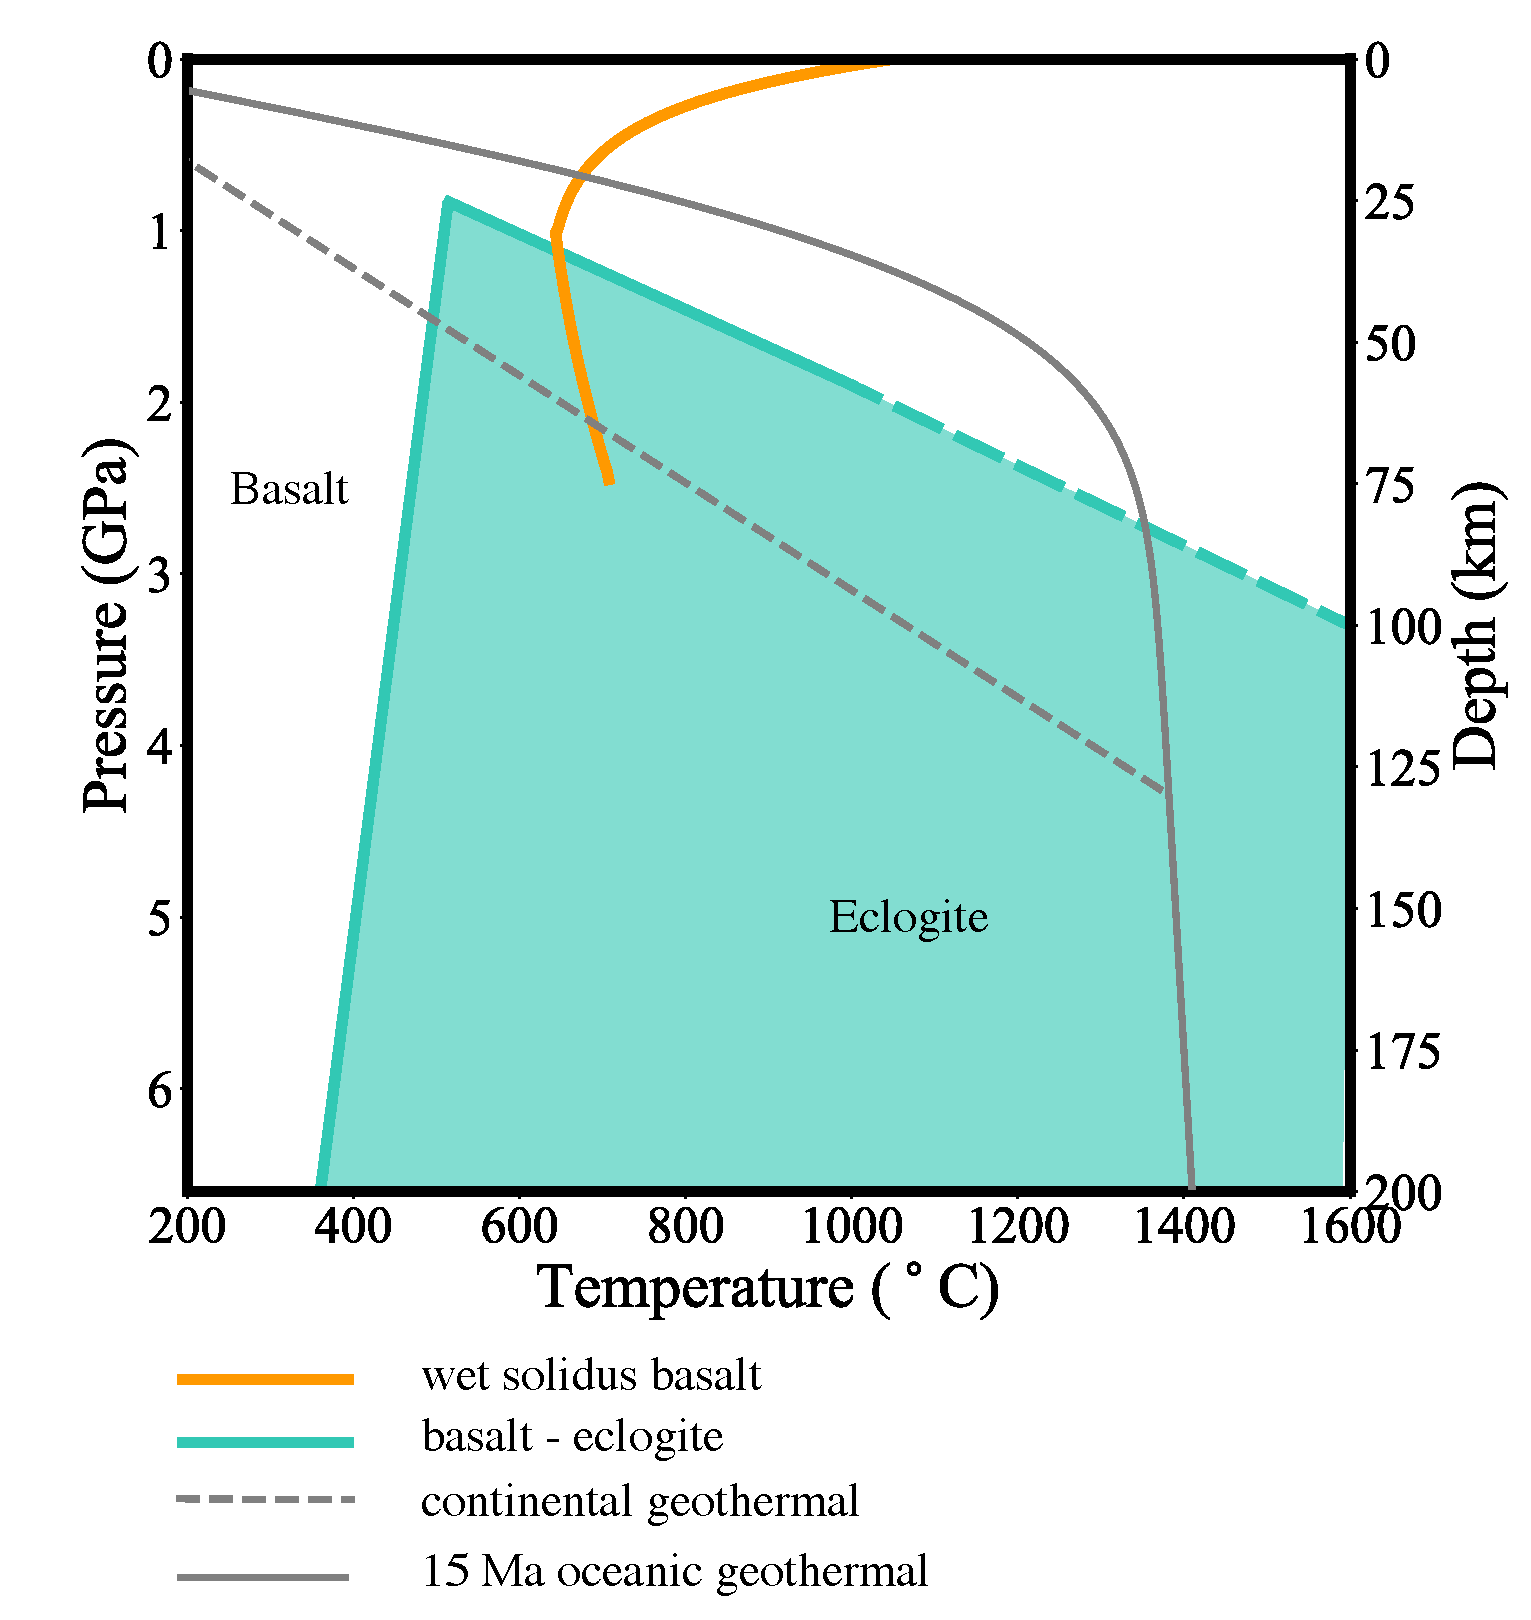
\includegraphics[width=4in]{basalt_phase_diagram_v1.pdf}
    \caption[鎂鐵質岩相圖,參考自\citet{Hacker2003}與\citet{Gutscher2000Bcan}]{鎂鐵質岩相圖,綠線隔開玄武岩與榴輝岩的穩定場,參考自\citet{Hacker2003},橘線為鎂鐵質岩的含水固相線,參考自\citet{Gutscher2000Bcan},綠虛線為外插值。}
    \label{fig::basalt_phase_diagram}
\end{figure*}

\subsection{沉積岩 --- 片岩}
模型中的沉積物在隱沒過程中進入高壓環境,發生成岩作用、壓密作用與變質作用。
不過由於這一系列作用是連續的,因此模型中的相變過程並不會造成岩石有大幅度物理性質上的改變。
下列方程為沉積物轉為片岩過程的條件式。
\begin{align}
T > 650\; {\rm ^\circ C}
\end{align}
本研究有考量沉積物的部分熔融,參考自\citet{van2011subduction}。
\begin{align}
    T > {\rm max} (578+ P \times 0.121,\ 617+e^{P\times 1.7\times 10^{-3}}) \; {\rm ^\circ C}
\end{align}
其中$P$為十億帕斯卡(GPa)。
圖\ref{fig::sediment_phase_diagram}為沉積物岩相溫壓相圖。
\begin{figure*}[ht!]
    \centering
    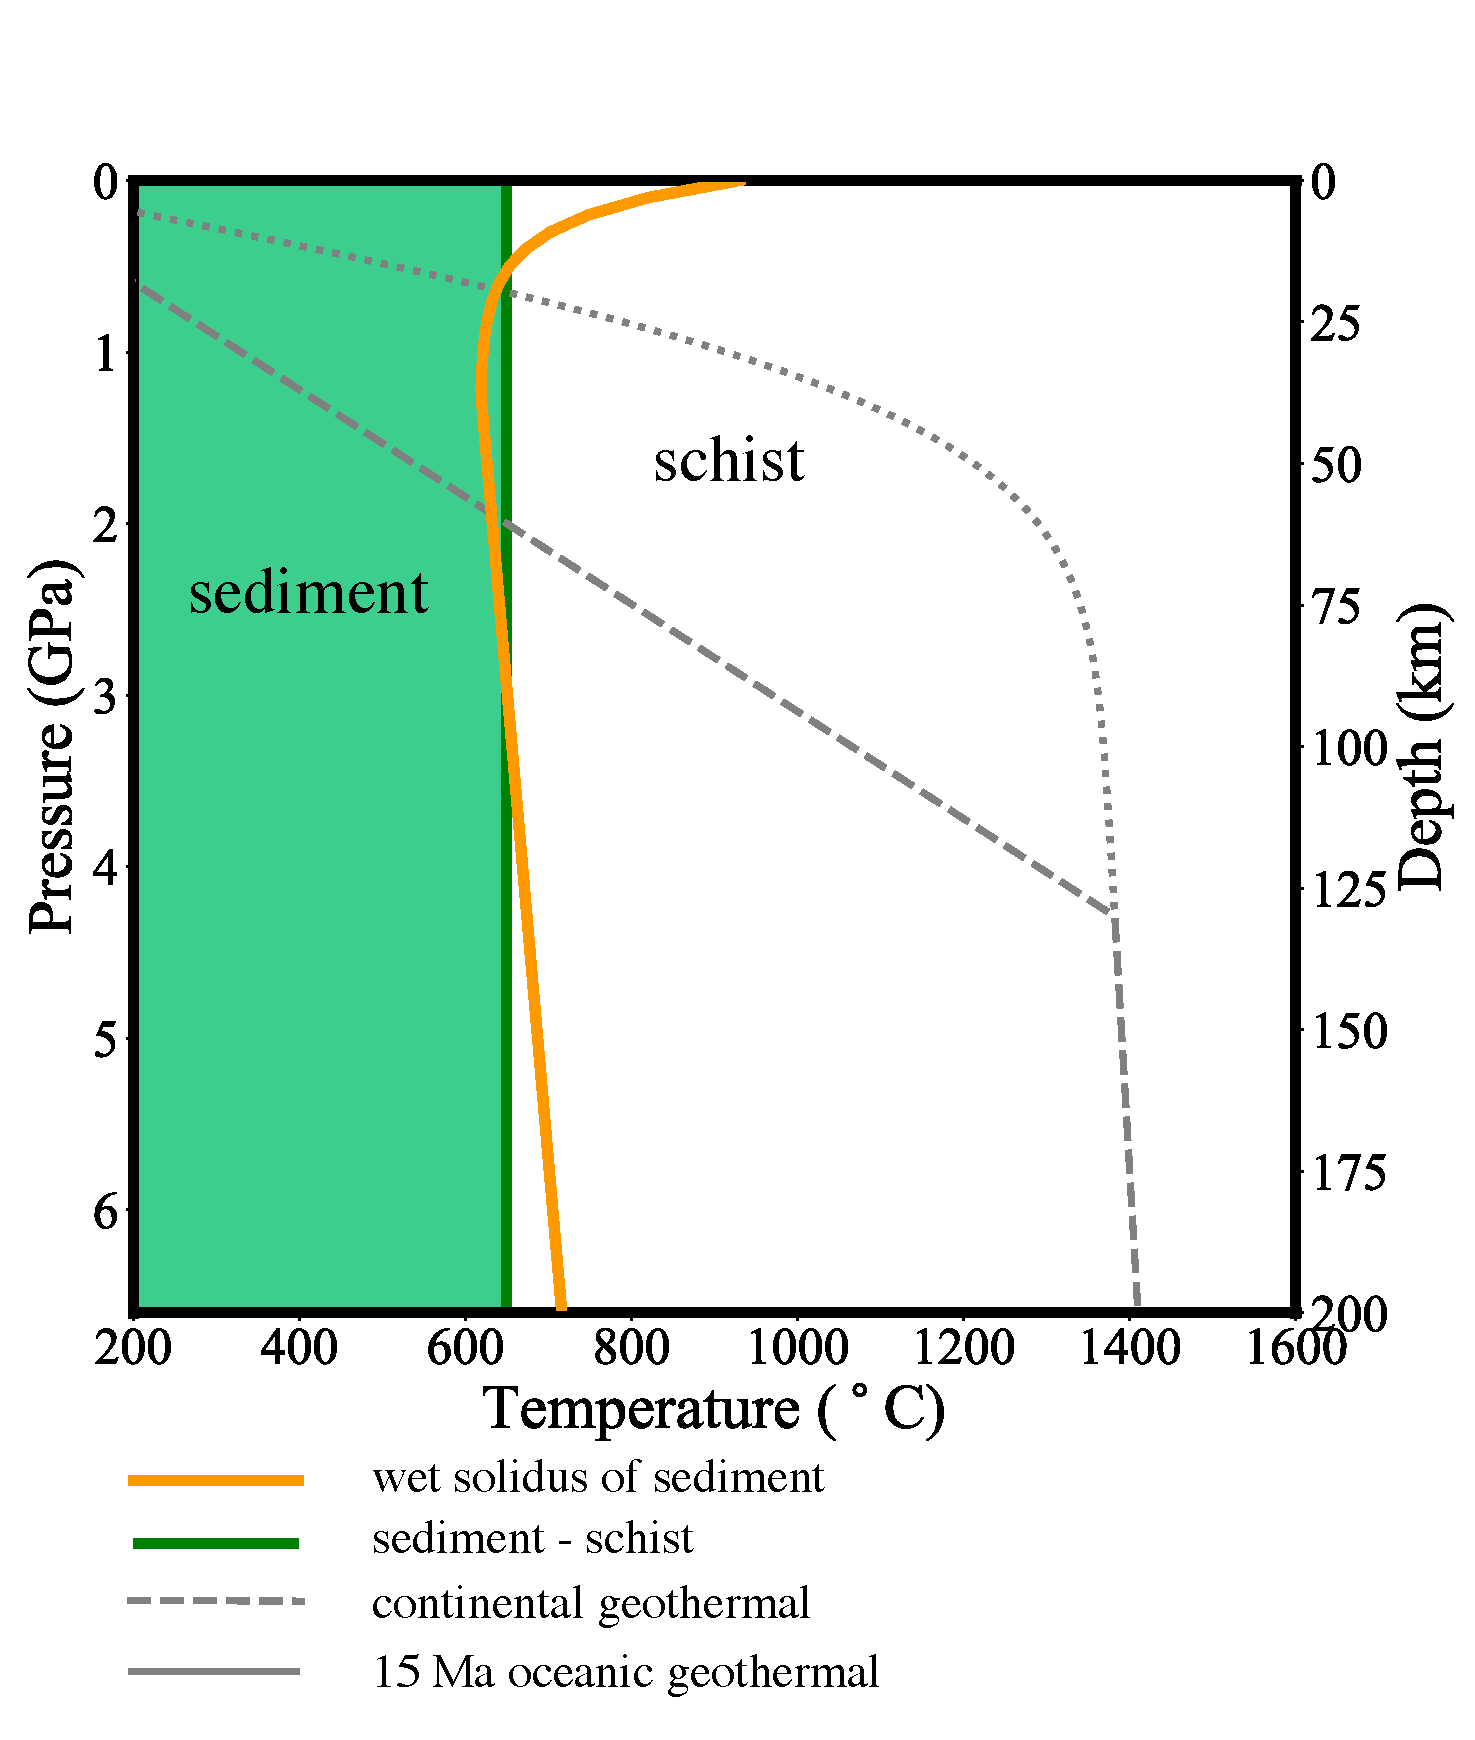
\includegraphics[width=4in]{sediment_phase_diagram_v1.pdf}
    \caption[沉積物變質岩相圖,參考自\citet{van2011subduction}]{沉積物變質岩相圖,橘線為沉積物含水固相線,參考自\citet{van2011subduction}。}
    \label{fig::sediment_phase_diagram}
\end{figure*}

\subsection{含綠泥石之橄欖岩 --- 橄欖岩}

模型中的地函除了普通橄欖石與蛇紋化橄欖石之外,還有考慮含綠泥石之橄欖岩的存在。
本研究假設部分熔融事件只會發生在具有含綠泥石之橄欖岩的海洋岩石圈上方的地函楔。
一旦溫度太高而使岩石脫水,含綠泥石之橄欖岩就會轉變為一般的橄欖石。
相變條件式參考自\citet{Grove2009},簡化式如下:
\begin{align}
T > 800-3.5\times 10^{-8}\times (P\times 3 \times 10^{4} -62)^{2} \; {\rm ^\circ C}
\end{align}
其中$P$為十億帕斯卡(GPa)。
圖\ref{fig::chlorite_phase_diagram}為含綠泥石之橄欖岩岩相圖。
\begin{figure*}[ht!]
    \centering
    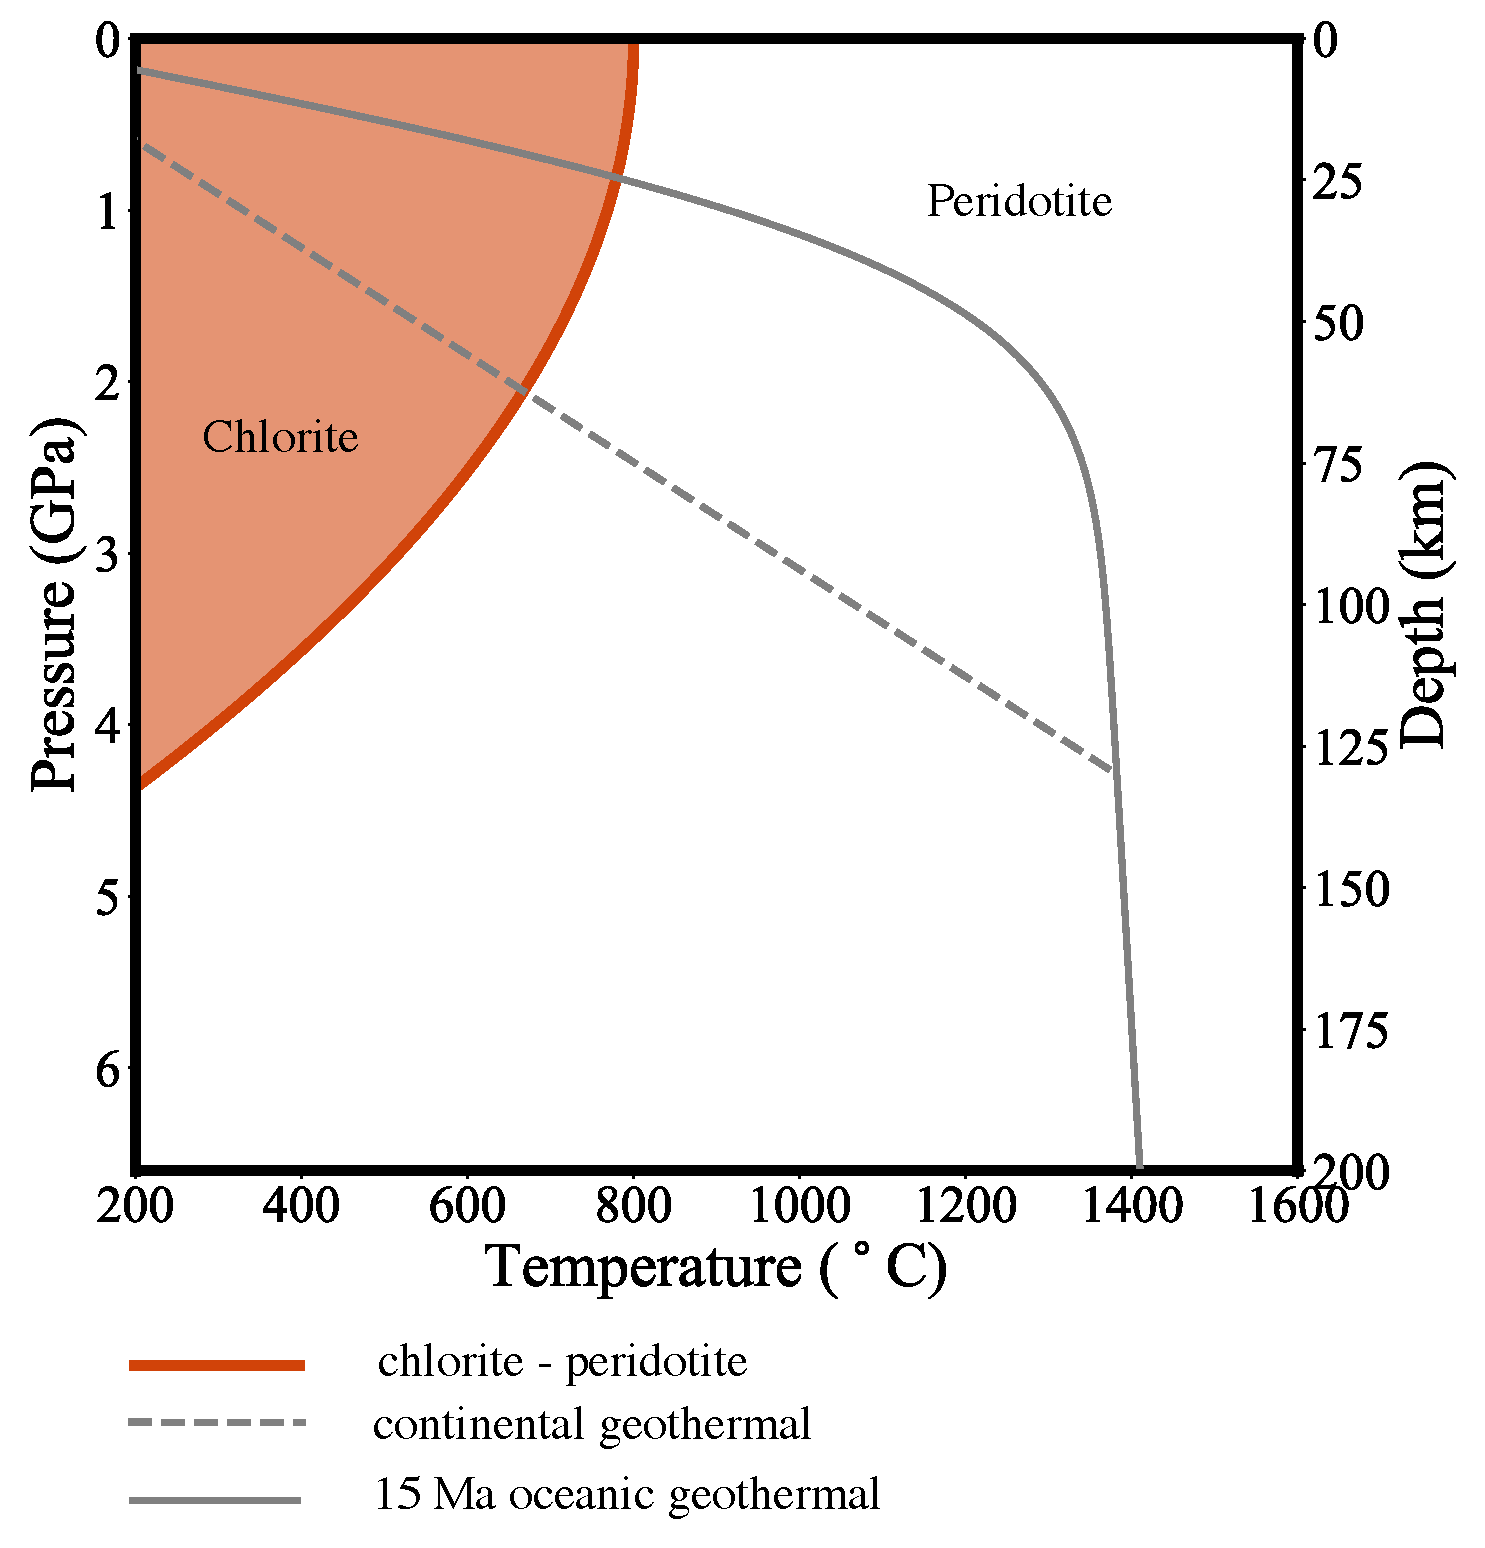
\includegraphics[width=4in]{chlorite_phase_diagram_v1.pdf}
    \caption[含綠泥石之橄欖岩岩相圖,參考自\citet{Grove2009}]{含綠泥石之橄欖岩岩相圖,橘紅線為含綠泥石之橄欖岩脫水相變線,參考自\citet{Grove2009}。}
    \label{fig::chlorite_phase_diagram}
\end{figure*}

\section{熱邊界條件}\label{熱邊界條件}
%\subsection{運動邊界條件}
%在現實自然界中,板塊水平移動的主要作用力為板塊拉力和洋脊推力兩個分量,
%為了方便控制隱沒系統的聚合速度,本研究數值模型會對模型邊界施加速度控制隱沒系統的聚合速度,此為模型運動邊界條件。
%而模型中板塊主要的驅動力則由運動邊界條件所施加的速度控制。

%於本研究中所使用的板塊水平移動運動起初由速度邊界條件所決定,在模型運算期間皆為不隨時間變化的常數,然而,真實自然界中板塊移動速度與時間的關係不應為常數。
%在本研究的智利模型中,所使用的速度邊界條件滿足現生板塊移動速度模型(\citealp{schellart2008global})。然而在墨西哥模型中,由於其隱沒板塊較為年輕、強度低,在聚合速率較快的情況下容易發生海洋板塊斷裂的情況,因此
%因此在模型進行一段時間後,模型邊界條件隨邊界所承受之總體力大小所決定。

%模型會先設定左右邊界最大可施加的力臨界值大小Fc,當模型進行一萬個迴圈後,若邊界承受的力大於初始所給定的力臨界值,則會將速度下降為原先的0.9倍;反之若邊界承受的力尚未達到給定的力臨界值,則速度會增加為原先的1.1倍。此時,每一萬個迴圈,模型運動邊界條件會重新調整一次,以符合觀測結果。因此當模型運行一段時間之後,邊界所承受的力會約略相等於初始條件所設定的力臨界值。

%\subsection{熱邊界條件}\label{熱邊界條件}
本節中,岩石圈定義為熱傳導邊界層,本研究的熱傳導邊界底部溫度為攝氏1330$^{\circ}$。
模型中海洋岩石圈溫度構造使用半空間冷卻模型(half space cooling model),海洋岩石圈厚度與岩石圈年紀之開根號呈正比。由 \citealp{davis1974}提出:
\begin{align}
T=T_0+(T_m-T_0)\cdot erf(\frac{z}{2\sqrt{\kappa t}}) \label{eq:Half Space Model}
\end{align}
$T$ 是溫度,$T_m$ 是地函溫度,在本研究中使用攝氏1330$^{\circ}$。
$z$ 是與地表的距離,單位是公里,$\kappa$ 是熱擴散系數,在本研究中使用$10^{-6} \frac{m}{s^2}$。$t$ 是海洋岩石圈年紀。

大陸板塊的溫度構造有雙層構造與單層構造之區別。
本研究根據墨西哥與智利過去的地球物理研究,分別對墨西哥模型與智利模型設定不同的大陸岩石圈溫度構造。

墨西哥模型中,大陸岩石圈為雙層構造,近地表每公里20度溫度梯度,直到深度至45公里之後溫度梯度為每公里6度,至溫度到達攝氏1330度後維持恆溫。
此溫度構造建立在過去墨西哥平坦隱沒區域溫度模型研究(\citealp{Manea2005}; \citealp{Manea2011Thermal}; \citealp{Manea2011Curie})所提供的約束。

智利模型中,大陸岩石圈地溫梯度是單層構造,以岩石圈底部深度140公里作為參考(\citealp{perez2008}),從地表攝氏0度到岩石圈底部攝氏1330度,中間進行線性內插,僅含單一地溫梯度,約略為每公里攝氏9.5度。

能量交換在岩石圈中以熱傳導為主,溫度變化極大,然而在軟流圈,熱能傳遞以對流為主,因此整個軟流圈至地函地核邊界(core mantle boundary)的溫度皆維持地函絕熱溫度,僅存在因密度變化所造成之絕熱溫度梯度,因此模型中將岩石圈底部溫度固定為地函絕熱溫度1330度。
不同構造區溫度隨深度變化圖見圖\ref{fig::geothermal}。
\begin{figure*}[ht!]
    \centering
    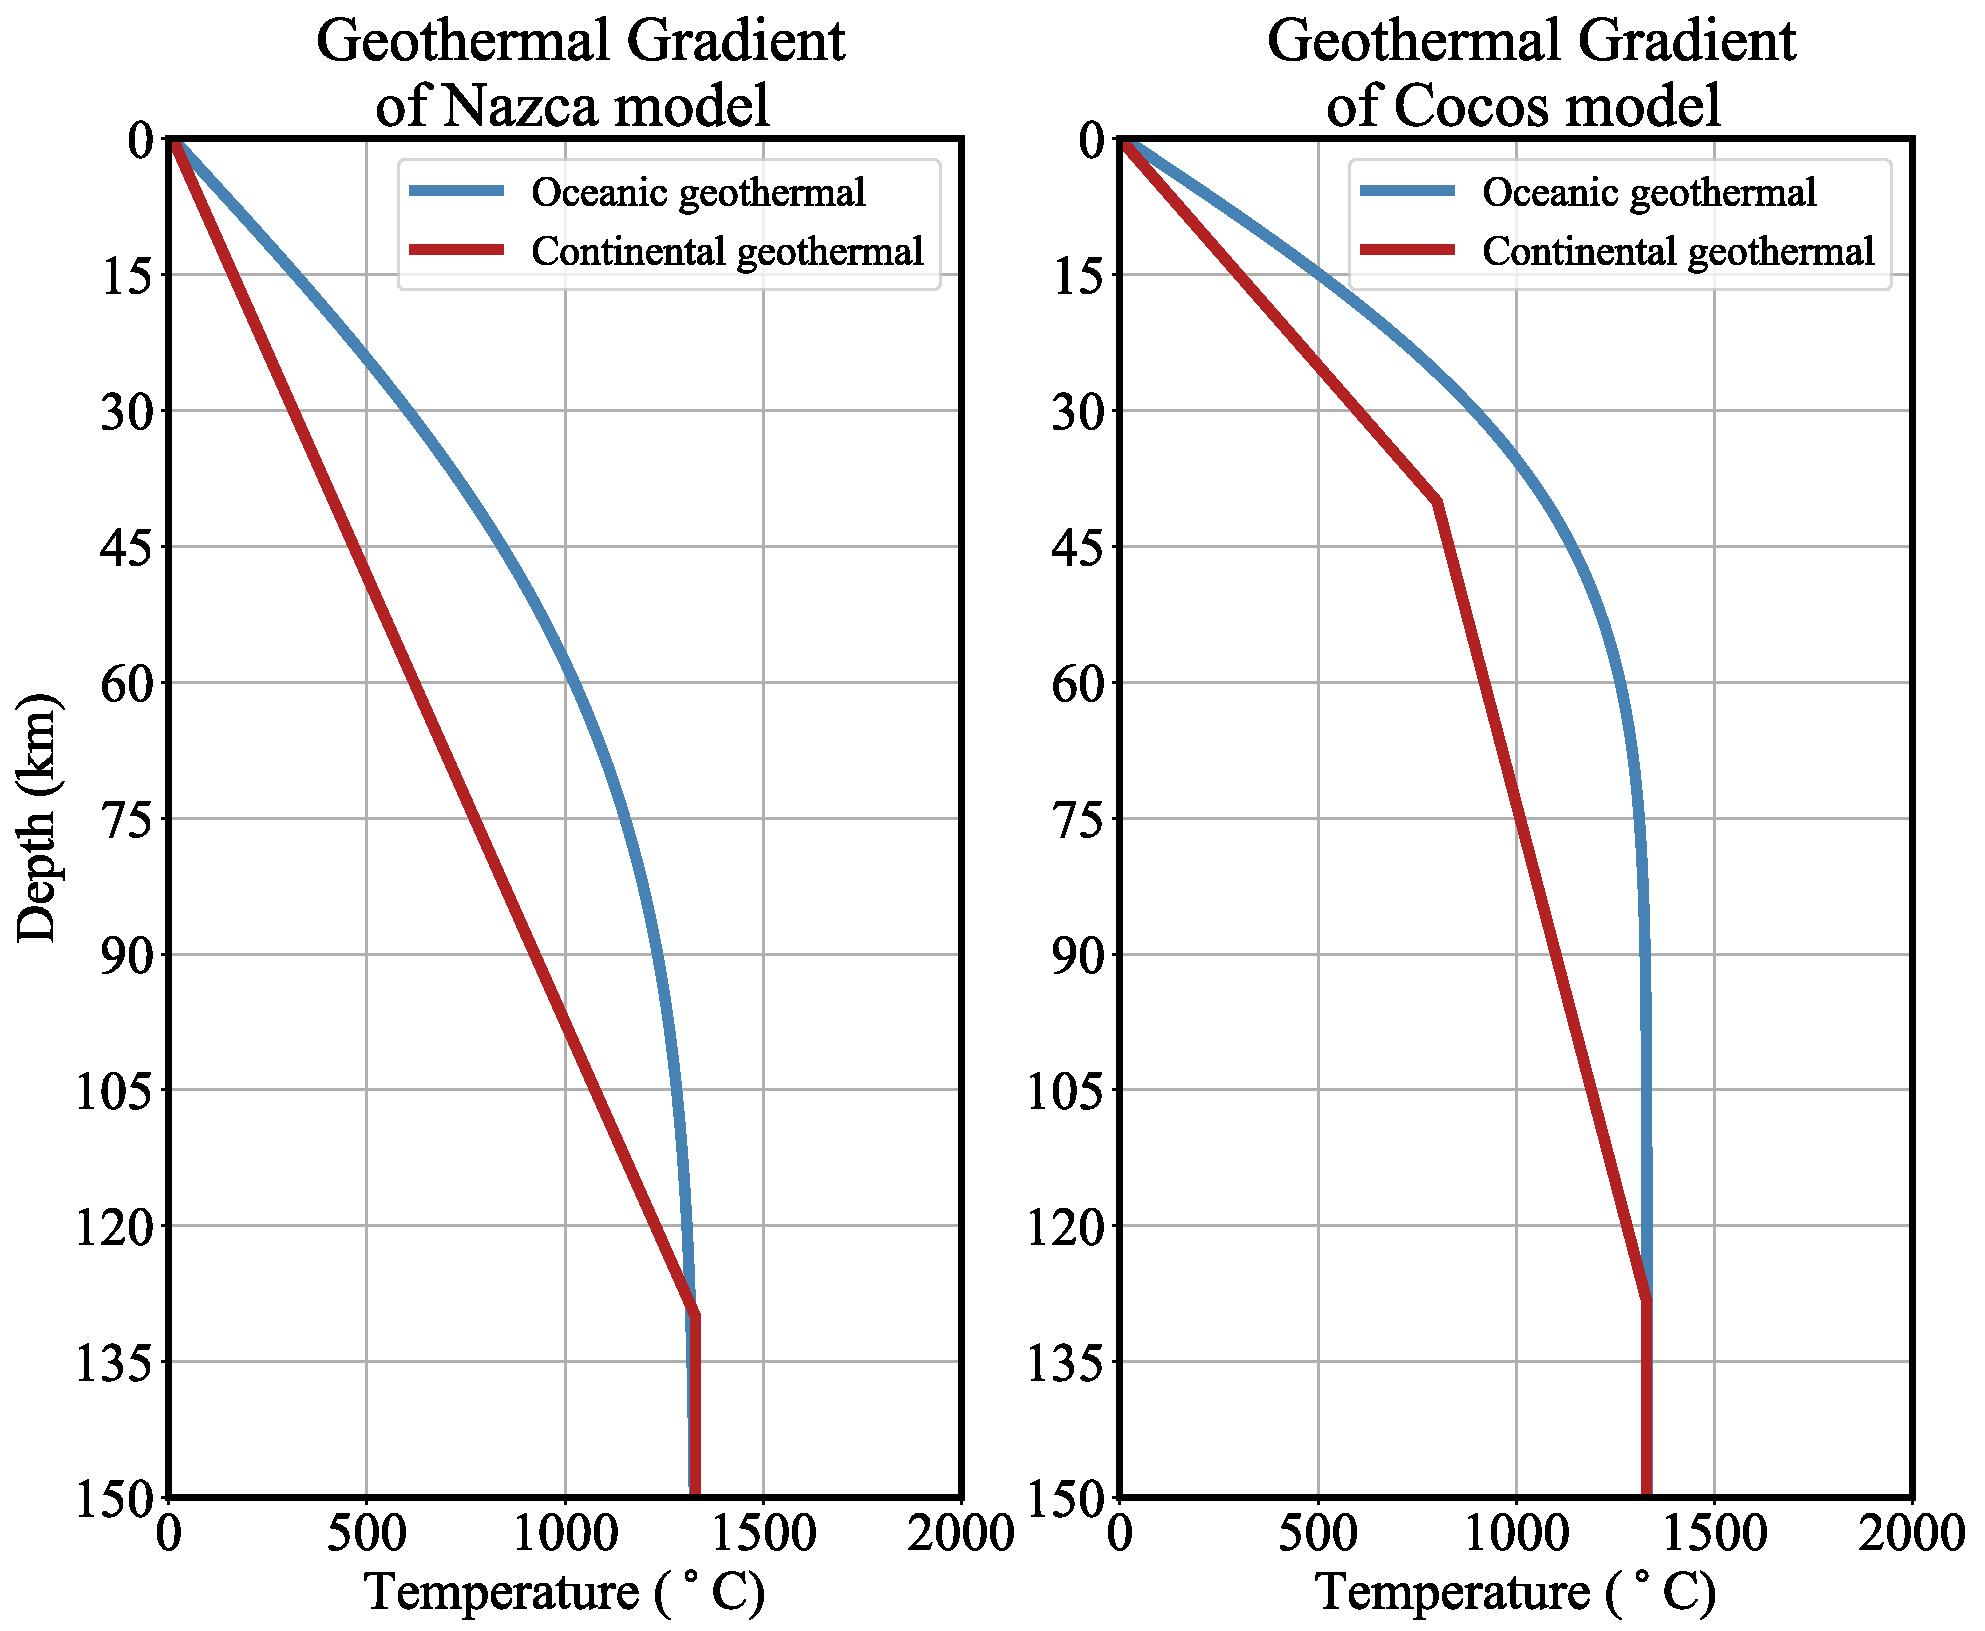
\includegraphics[width=5.5in]{temperature_profile_v2.pdf}
    \caption[本研究使用之模型地下溫度剖面圖]{本研究使用之模型地下溫度剖面圖,左圖為智利模型,右圖為墨西哥模型。藍色實線為海洋岩石圈地溫梯度,由式\ref{eq:Half Space Model}與海洋岩石圈年紀決定。咖啡色實線為大陸岩石圈地溫梯度,智利模型大陸岩石圈為單層構造,墨西哥模型大陸岩石圈為雙層構造。圖中並沒有考量絕熱地溫梯度。}
    \label{fig::geothermal}
\end{figure*}


\section{地表侵蝕}
地表地形演化與板塊構造活動有高度相關,在本研究模型中利用較簡單的方式模擬地形演化過程,包含侵蝕與沉積物堆積作用,使用一維擴散方程式控制侵蝕與堆積作用的速率,最早由\citealp{culling1960analytical} 所提出,其方程式如下:
\begin{align}
\frac{\partial z}{\partial t} = \kappa_S \nabla^2 z \label{eq:erosion}
\end{align}
其中$z$為模型中地表節點高度,其數學意義為對地表高度進行二次導數後得到該點曲率,並照曲率大小對其進行地形下修與上修,地形較突出處會被侵蝕,反之地形凹陷處容易被侵蝕物所堆積。物理意義則為守恆公式之展現,將地形假想為一二維空間方程式,在地形上每一點會因重力而有往下流動物質通量S,流動物質通量與地形坡度呈正比:
\begin{align}
\vec S = -k\nabla \vec z \label{eq:S}
\end{align}
其中$k$為正比係數。並且由於物質永遠守恆,在滿足守恆公式的假設下,物質質量不隨時間變化,令物質質量與時間的關係式:
\begin{align}
\rho\frac{\partial z}{\partial t}\label{eq:rho}
\end{align}

質量隨時間的變化會等同於物質在空間中的通量,因此式($\ref{eq:S}$) 與式($\ref{eq:rho}$) 的關係如下:
\begin{align}
\rho\frac{\partial z}{\partial t} = -\vec\nabla\cdot \vec S = -\vec\nabla \cdot (-k\nabla \vec z)\label{eq:erosion2}
\end{align}
或
\begin{align}
\frac{\partial z}{\partial t} = \frac{k}{\rho}\nabla^2 z\label{eq:erosion3}
\end{align}
令$\frac{k}{\rho}=\kappa_S$,其中$\kappa_S$為坡度擴散係數,本研究中侵蝕與堆積的坡度擴散係數相同,單位為$\frac{m^2}{s}$。可得:
\begin{align}
\frac{\partial z}{\partial t} = \kappa_S\nabla^2 z\label{eq:erosion4}
\end{align}

\section{岩漿作用}\label{岩漿作用}
本研究的數值模型包含隱沒帶中的岩漿作用。
隱沒板塊進入地函時,其上覆沉積物與玄武岩在進入高溫高壓環境的同時發生脫水與相變。
當水分進入地函楔中,其固相線(solidus)從乾固相線移動至含水固相線,隱沒板塊上方的橄欖岩熔點大幅降低。
地溫梯度因此容易經過含水固相線,發生部分熔融事件,隨後產生岩漿,部分岩漿分佈在地函與地殼中,成為岩漿庫(magma chamber),而剩餘岩漿噴發至地表形成火山島弧(volcanic arc)。

\begin{figure*}[ht]
    \centering
    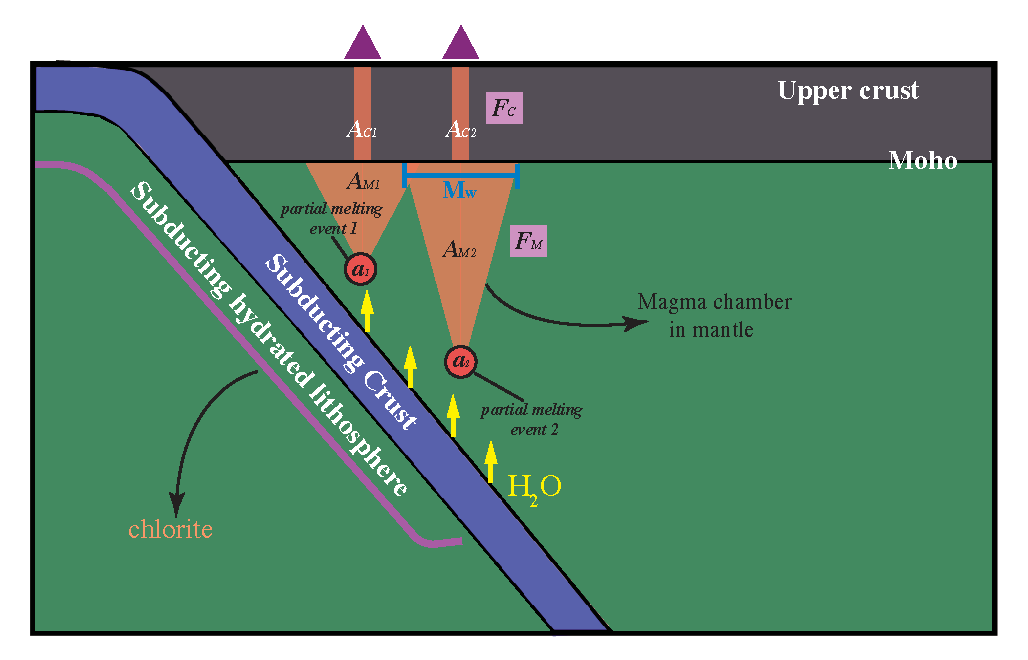
\includegraphics[width=6in]{melting.pdf}
    \caption[模型內岩漿作用示意圖。]{模型內岩漿作用示意圖。圖中繪製兩個不同的部分熔融事件。每個獨立部分熔融事件會對應獨立的岩漿庫。
    模型中有F$_M$比例的岩漿留在地函楔中,F$_C$比例的岩漿留在地殼中,其餘1-F$_M$-F$_C$比例的岩漿會噴發至地表形成火山島弧,如圖上方紅紫色三角形。
    地函岩漿庫中的岩漿均勻分布在圖中地函楔中紅橘色倒三角形。
    圖中假設部分熔融事件二的部分熔融體積為a$_2$地函岩漿庫體積為A$_{M2}$。
    }
    \label{fig::melting}
\end{figure*}

\subsection{部分熔融}\label{部分熔融}
本研究共考慮三種岩相的部分熔融,分別為在地函楔中的橄欖岩相(包含橄欖岩與蛇紋岩)、沉積岩相與鐵鎂質岩相(包含玄武岩與榴輝岩),並且假設最大部分熔融體積為總體網格內的10$\%$。
當上述三種岩相之標記點通過\ref{相變}節中提及之固相線後,便將該標記點視為熔融態,部分熔融比例($p_{melt}$)計算方式如下:
\begin{align}
    p_{melt}=\frac{(T-T_{solidus})}{500}\times 10\% \label{eq:melting}
\end{align}

其中$T_{solidus}$為該標記子深度下對應至固相線的溫度,即為熔點(melting point),部分熔融比例在熔點與高於熔點500度範圍內從0$\%$線性增加至10$\%$。
模型中允許多個部分熔融事件發生,並且會依照部分熔融比例累加,隨後藉由部分熔融比例計算模型中的岩漿量。

\subsection{岩漿庫}\label{岩漿庫}
本研究假設有F$_M$比例的岩漿留在地函楔中,F$_C$比例的岩漿留在地殼中,其餘1-F$_M$-F$_C$比例的岩漿會噴發至地表。
留在地函楔中的岩漿成為岩漿庫,部分熔融發生後,模型中假設從熔點開始產生一倒三角形的地函岩漿庫,假設地函岩漿庫頂部皆在莫荷面下,並在莫荷面處達到最大寬度$M_W$公里,如圖\ref{fig::melting}所示,該最大寬度與岩漿往左右移動的流動性有關,本研究中所有模型一律將最大寬度設為50公里。
由於本研究並沒有探討地殼中岩漿對模型動力的影響,因此地殼中的岩漿庫一律視為一垂直莫荷面的柱狀岩脈。

岩漿庫中每個網格的體積融化比例(M)為與時間相關的函數,每個部分熔融事件所產生的岩漿會在模型中累積。
每個時間點的體積融化比例分為每個時間點產生的岩漿量與每個時間點冷卻的岩漿量,由下式表示:
\begin{align}
    M(t+dt)-M(t) = \Delta M = Pdt-M(t)\lambda dt \label{eq:Magma}
\end{align}
\begin{align}
    P = P_0 \times p_{melt} \times F_M \times A \label{eq:Magma P}
\end{align}
\begin{align}
    \lambda = \lambda_0\times exp(-\lambda_T \times \Delta T) \label{eq:Magma lambda}
\end{align}
式\ref{eq:Magma}中,$Pdt$項為每時間點岩漿產生量,與部分熔融比例有關,$P$為岩漿產生速率。
$M(t)\lambda dt$為每時間點岩漿冷卻量(岩石結晶量),與岩漿庫大小有關,$\lambda$為岩漿冷卻速率。
式\ref{eq:Magma P}計算岩漿產生速率,$P_0$是岩漿產生常數,單位為$m^3/m/s$,亦即每海溝截面所產生的岩漿體積速率。
$p_{melt}$來自式\ref{eq:melting},為部分熔融百分比。
A為發生部分熔融的體積比例,地函中的A為發生部分熔融體積與預設岩漿庫倒三角形的總面積比值,以圖\ref{fig::melting}的部分熔融事件二而言,A = (部分熔融發生面積 a$_2$/倒三角形面積 A$_{M2}$),地殼中的A = (部分熔融發生面積a$_2$/地殼岩脈面積A$_{C2}$)。
$\Delta T$為包含岩漿的網格與周遭網格的溫度差,溫度差越高(亦即周遭網格溫度越低),則岩漿冷卻速率越快。
式\ref{eq:Magma lambda}描述岩漿冷卻參數$\lambda$,$\lambda_0$為岩漿冷卻衰變常數,$\lambda_T$是與溫度有關的冷卻係數,單位為$\frac{1}{K}$。

岩漿量的變化意味著岩石的物態改變。
物質的物態改變在溫度相同的情形下會有能量的吸收或釋放,本研究有考慮岩漿量變化過程中的能量變化。
\subsection{岩漿作用造成的溫度影響}\label{岩漿作用造成的溫度影響}
本研究只考慮在岩漿結晶過程中所釋放的潛熱(放熱)。
模型中會計算每個時間的岩漿變化量($\Delta M$),估計岩漿結晶冷卻中釋放的能量與其所造成的溫度變化量,使用公式如下:
\begin{align}
    T(t+dt) = T(t) + M(t+dt)\times \lambda \times dt \times \frac{L_H}{C_p}\label{eq:latent heat}
\end{align}
其中$L_H$為岩漿潛熱值,在本研究使用安山岩漿的潛熱值$3\times 10^5$ J/kg(\citealp{liu2011modeling})。
$C_p$為等壓比熱容量。

當岩漿結晶後,周遭岩石的溫度因放熱而有局部升高的現象,該過程會些微影響地函楔中的黏滯度與隱沒帶動力過程。

\section{計算數值模型中的轉動力矩}\label{計算數值模型中的轉動力矩}
本研究利用數值解的結果計算模型中不同時間點,在假設海溝為支點的情況下,獲得隱沒板塊所受的重力力矩與動水壓力力矩。
本研究所使用重力力矩數值求解式如下:
\begin{align}
    \tau_{gravity} =  g\sum ^L_{l=0} \Delta \rho(l)\ r(l)\ cos\ \alpha (l)\ V(l) 
    \label{eqn:tau_gravity}
\end{align}
整段隱沒板塊被切割成$l$段板塊,每段$l$皆有個別的密度差$\Delta \rho(l)$、力臂(moment arm)為$r(l)\ cos\ \alpha (l)$與體積$V(l)$。
其中$r(l)$為從支點到$l$段中心點的直線距離,$ \alpha (l)$為$r(l)$與重力的夾角,亦即$r(l)$與垂直方向上的夾角,故$r(l)\times cos\ \alpha (l)$為轉動系統中的力臂。
體積$V(l)$由隱沒板塊上攝氏800$^{\circ}$等溫線以內範圍所決定。

本研究所使用動水壓力力矩數值求解式如下:
\begin{align}
    \tau_{suction} =  \sum ^L_{l=0} [P_{sub}(l)-P_{wedge}(l)]\cdot dl \cdot cos\ \beta(l)\cdot r(l)\ 
    \label{eqn:tau_suction}
\end{align}
與重力力矩計算方法雷同,將隱沒板塊切割成$l$段,計算直接垂直於每段$l$上下的模型動水壓力差與$dl$段的乘積獲得作用在隱沒板塊上的壓力梯度力,並且再乘上$dl$段與力臂的夾角$\beta(l)$獲得作用力垂直作用於力矩上的實際大小。
最後計算壓力梯度力與力臂的乘積便為每段$l$所受的動水壓力力矩。

積分每段$l$所造成的轉動重力力矩與動水壓力力矩後便可得該時間點下的總重力力矩與總動水壓力力矩,由於本研究為二維模型,單位皆為N$\cdot$ m/m。


\begin{landscape}
\begin{table}[htp]\large
    \caption[模型中岩石參數列表,參考自\citet{ranalli1995rheology}]{模型中岩石參數列表,參考自\citet{ranalli1995rheology}。}
    \renewcommand{\arraystretch}{1.5}
    \centering
    \begin{tabular}{m{5.5cm}m{2cm}m{2cm}m{2.4cm}m{2.3cm}m{1cm}m{1cm}m{1.7cm}m{1.7cm}}
        \hline
        Material                                                                                    & \begin{tabular}[c]{@{}l@{}}Density\\ (kg m$^{-3}$)\end{tabular} & n    & \begin{tabular}[c]{@{}l@{}}A\\ (MPa$^{-n}$s$^{-1}$)\end{tabular} & \begin{tabular}[c]{@{}l@{}}E\\ J$\cdot$ m\textasciicircum{}\{-3\}\end{tabular} & \begin{tabular}[c]{@{}l@{}}$\phi_0$\\ ($^{\circ}$)\end{tabular} & \begin{tabular}[c]{@{}l@{}}$\phi_1$\\ ($^{\circ}$)\end{tabular} & \begin{tabular}[c]{@{}l@{}}$C_0$\\ Pa\end{tabular} & \begin{tabular}[c]{@{}l@{}}$C_1$\\ Pa\end{tabular} \\ \hline
        basalt                                                                                      & 2880                                                            & 3.05 & 1.25$\times$10$^{-1}$                                                          & 3.76$\times$10$^5$                                                                         & 30                                                              & 15                                                              & 4$\times$10$^7$                                                & 4$\times$10$^6$                                                 \\
        eclogite                                                                                    & 3480                                                            & 3.05 & 1.25$\times$10$^{-1}$                                                          & 4.5$\times$10$^5$                                                                          & 30                                                              & 15                                                              & 4$\times$10$^7$                                                & 4$\times$10$^6$                                                 \\
        continental upper crust                                                                     & 2800                                                            & 3.05 & 1.25$\times$10$^{-1}$                                                          & 2.76$\times$10$^5$                                                                         & 30                                                              & 15                                                              & 4$\times$10$^7$                                                & 4$\times$10$^6$                                                 \\
        \begin{tabular}[c]{@{}l@{}}continental lower crust/ arc\\ (strong lower crust)\end{tabular} & 2900                                                       & 3.05 & 1.25$\times$10$^{-1}$                                                          & 5.76$\times$10$^5$                                                                         & 30                                                              & 15                                                              & 4$\times$10$^7$                                                & 4$\times$10$^6$                                                 \\
        \begin{tabular}[c]{@{}l@{}}continental lower crust \\ (weak lower crust)\end{tabular}       & 2900                                                            & 3.05 & 1.25$\times$10$^{-1}$                                                             & 2.76$\times$10$^5$                                                                         & 30                                                              & 15                                                              & 4$\times$10$^7$                                                & 4$\times$10$^6$                                                 \\
        sediment                                                                                    & 2800                                                            & 3    & 5$\times$10$^2$                                                              & 2$\times$10$^5$                                                                            & 3                                                               & 3                                                               & 4$\times$10$^6$                                                & 4$\times$10$^6$                                                 \\
        schist                                                                                      & 2900                                                            & 3    & 7$\times$10$^4$                                                              & 3.76$\times$10$^5$                                                                         & 30                                                              & 15                                                              & 4$\times$10$^7$                                                & 4$\times$10$^6$                                                 \\
        mantle (perdiotite)                                                                         & 3300                                                            & 3    & 7$\times$10$^4$                                                              & 5.2$\times$10$^5$/ 4.95$\times$10$^5$                                                                      & 30                                                              & 15                                                              & 4$\times$10$^7$                                                & 4$\times$10$^6$                                                 \\
        serpentinite                                                                                & 3200                                                            & 3    & 7$\times$10$^4$                                                              & 1.2$\times$10$^5$                                                                          & 3                                                               & 3                                                               & 4$\times$10$^6$                                                & 4$\times$10$^6$                                                 \\
        chlorite                                                                                    & 3300                                                            & 3    & 7$\times$10$^4$                                                              & 5.2$\times$10$^5$                                                                          & 30                                                              & 15                                                              & 4$\times$10$^7$                                                & 4$\times$10$^6$                                                 \\ \hline
    \end{tabular}
\label{table::phase_table}
\footnotesize 所有岩石的熱傳導係數(thermal conductivity) = 3.3 Wm$^{-1}$$^{\circ}$C$^{-1}$,比熱容(heat capacity) = 10$^3$J $\cdot$kg$^{-1} \cdot$ K$^{-1}$,熱膨脹係數(thermal expansion) = 5 $\times$ 10 $^{-5}$ K $^{-1}$
\end{table}
\end{landscape}
% !TeX root = ../main.tex

\chapter{數值模型結果}

\section{智利參考模型}
\subsection{初始模型設定}
本研究建立一個長1200公里、深300公里的長方形二維剖面,包含一段長425公里的海洋岩石圈與775公里的大陸板塊,在兩個板塊交界處,建立一段長度31公里傾角35度的隱沒板塊,交接處區域的溫度較高,方便隱沒帶發育。
智利參考模型設計見圖\ref{fig::reference Nazca model}。
海洋岩石圈年齡為40個百萬年(\citealp{muller2019}),包含2公里厚的沉積物、6公里厚的玄武岩與10公里厚的綠泥岩,其熱構造由第二章式\ref{eq:Half Space Model}提及的半空間冷卻模型決定。

\begin{figure*}[hb]
    \centering
    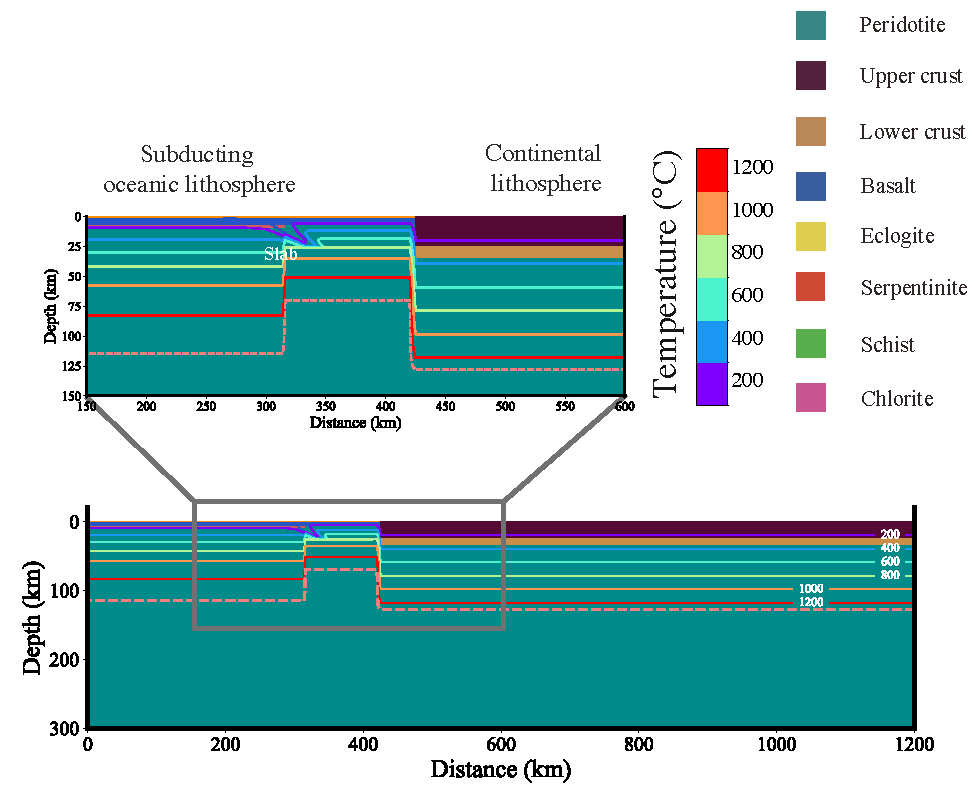
\includegraphics[width=6in]{Ref_Nazca.pdf}
    \caption[智利參考模型設計與邊界條件示意圖]{智利參考模型設計與邊界條件示意圖}
    \label{fig::reference Nazca model}
\end{figure*}

大陸岩石圈包含25公里厚的上部地殼(upper crust)與10公里厚的下部地殼(lower crust),由於秘魯與智利平坦隱沒區域的大陸地溫梯度資料較少,過去研究並沒有很好的約束,僅透過重力資料推測彈性岩石圈厚度大約140公里,因此模型設定地溫梯度以每公里攝氏9.5$^{\circ}$線性遞增至140公里深(\citealp{perez2008})至岩石圈底部1330$^{\circ}$。
地表溫度皆為攝氏10$^{\circ}$,模型底部溫度固定攝氏1330$^{\circ}$。

由於現生地震學觀測研究提及該地區地震活動度大,且地函岩石圈速度較高、板塊脫水作用不活躍,因此智利參考模型的蛇紋岩厚度參數設定為5公里。模型左邊界從地表至300公里深皆以等速率每年6公分往右移動,右邊界則固定不動。
本研究速度參考來自於\citealp{o2005uncertainties},使用印度-大西洋熱點參考座標(Indo-Atlantic hotspot reference frame)中的相對板塊運動模型計算(\citealp{schellart2008global})。

模型上邊界為自由表面,而下邊界則為開放邊界,物質可自由進出。
需要注意現今的秘魯與智利平坦隱沒區皆落在安地斯山脈造山範圍,然而本參考模型沒有包含造山運動。
就現今觀測資料來看,平坦隱沒事件早於安地斯造山事件(\citealp{chen2019southward}; \citealp{hu2021southward}),兩者並沒有直接關係。


\subsection{智利參考模型結果}\label{智利參考模型結果}
智利參考模型產生一深度約100-110公里、長度約300公里的平坦段。

在隱沒初始時期,隱沒作用促使地函流上湧,導致地函楔溫度升高,同時強烈的岩石變形與破壞導致隱沒板塊交界處產生摩擦熱,海洋地殼溫度被動上升。
岩石在一系列的加溫下發生相變,隱沒地殼上的玄武岩相在約攝氏500$^{\circ}$等溫線(深度40公里處)處相變成緻密的榴輝岩相,如圖\ref{fig::Nazca_Ref_26}a所示。
榴輝岩相密度遠大於周遭地函密度,顯著的密度差造成隱沒系統中的重力不穩定,促使隱沒板塊驅動力產生,隱沒系統得以順利發育,隱沒帶密度剖面見圖\ref{fig::Nazca_Ref_26}c。

海洋地殼上的沉積物在隱沒過程中絕大比例在海溝處堆積,形成厚度約10公里的增積岩體,僅有少部分沉積物被帶入地函中,這些沉積物與海水隨著地殼進入高溫高壓環境。
離開近地表後,地殼上的黏土礦物逐漸進入不穩定狀態,釋放出晶格中的水分,導致地函楔中的橄欖岩發生水合作用(hydration reaction)而相變成蛇紋岩化的橄欖岩(serpentinized peridotite),其與隱沒的沉積物一同在地函楔中形成強度低且密度較低的低黏滯度通道(low viscosity channel),見圖\ref{fig::Nazca_Ref_26}b與圖\ref{fig::Nazca_Ref_51}b模型黏滯度剖面。

在地函較深處,蛇紋岩化的橄欖岩進入更高溫的環境發生脫水,於深度70公里處相變回橄欖岩。
由於70公里深的環境已達到攝氏700$^{\circ}$,岩石幾乎都以黏性變形為主,因此低黏滯度通道在蛇紋岩化橄欖岩脫水後依然存在於板塊交界處中。

海洋板塊中的綠泥岩在120-130公里深處發生脫水,相變成普通的橄欖岩。
儘管綠泥岩脫水作用導致地函楔中的熔點下降,然而隱沒早期板塊溫度較低,即便進入地函楔中依然難以達到岩石熔點。

隱沒早期強烈的聚合作用在大陸岩石圈攝氏600$^{\circ}$等溫線之上方產生一厚度25公里、寬度150公里的高壓帶,詳見圖\ref{fig::Nazca_Ref_26}d動態壓力剖面紅色區域。
該高壓帶在10 Myr便不復存在,隨著隱沒持續進行,低黏滯度通道的存在隔絕上覆板塊、隱沒板塊與地函楔之間的物質交換,地函流
地函楔頂部、板塊交界處壓力降低,於80-120公里深處形成低壓區,見圖\ref{fig::Nazca_Ref_51}d深藍色區域。 
低壓區域促使動水壓力力矩增加,超過重力力矩,在模型隱沒系統中形成一逆時針方向上的轉動,直接促使隱沒板塊傾角(dip)快速降低(見圖\ref{fig::Nazca_Ref_slab_time})。

隨著隱沒板塊傾角降低,其下方因承受強烈彎曲(bending),在模型時間10-15 Myr之間於地函楔低壓區下方、隱沒地函岩石圈(subducting mantle lithosphere)處形成另一寬度約100公里的高壓區,見圖\ref{fig::Nazca_Ref_76}d紅色區域。
隱沒板塊下方的高壓帶與隱沒板塊上方的低壓帶平行於隱沒板塊,在隱沒板塊上
產生壓力梯度力,該力垂直作用於隱沒板塊。
在轉動系統中,壓力梯度力造成該隱沒段於逆時針方向上的力矩急遽增大,見圖\ref{fig::Nazca_Ref_torque_time},因此在模型時間15 Myr後形成平坦隱沒。

這段時間內因隱沒傾角漸緩,地函楔橄欖岩在壓力不變的情形下溫度逐漸上升,有部分岩石通過固相線,發生些許部分熔融事件,部分熔融位置於圖\ref{fig::Nazca_Ref_76}c中黃線處,部分熔融比例見圖\ref{fig::Nazca_Ref_melting_time}(a)。

隨後模型至30 Myr,平坦隱沒持續發育,其深度大致與原先大陸岩石圈攝氏800$^{\circ}$等溫線深度相同,在模型中約略100-120公里深(圖\ref{fig::Nazca_Ref_76}a、\ref{fig::Nazca_Ref_101}a、\ref{fig::Nazca_Ref_126}a、\ref{fig::Nazca_Ref_150}a)。
隱沒板塊在達到攝氏900$^{\circ}$等溫線前後離開平坦段,在深度120公里之後形成一高角度隱沒板塊。

因低黏滯度通道狹窄,隔絕地函流進入地函楔中,因此隱沒板塊上方的黏滯度持續維持低壓狀態。
此外,平坦隱沒上凹區域因強烈彎曲形成高壓帶,與板塊上方地函低壓帶形成的壓力梯度同樣垂直於隱沒板塊,因此在20 Myr之後,與重力力矩相比,動水壓力力矩維持穩定優勢,隱沒板塊與上覆板塊被牢牢吸住(圖\ref{fig::Nazca_Ref_76}b, d、\ref{fig::Nazca_Ref_101}b, d、\ref{fig::Nazca_Ref_126}b, d、\ref{fig::Nazca_Ref_150}b, d)。


\begin{figure*}[htp]
    \centering
    \includegraphics[width=6in]{Ref_Nazcaframe_26_snapshot_5field_200_v1.pdf}
    \caption[智利參考模型於5 Myr時之結果。]{智利參考模型於5 Myr時之結果。}
    \label{fig::Nazca_Ref_26}
\end{figure*}

\begin{figure*}[htp]
    \centering
    \includegraphics[width=6in]{Ref_Nazcaframe_51_snapshot_5field_200_v1.pdf}
    \caption[智利參考模型於10 Myr時之結果。]{智利參考模型於10 Myr時之結果。}
    \label{fig::Nazca_Ref_51}
\end{figure*}

\begin{figure*}[htp]
    \centering
    \includegraphics[width=6in]{Ref_Nazcaframe_76_snapshot_5field_200_v1.pdf}
    \caption[智利參考模型於15 Myr時之結果。]{智利參考模型於15 Myr時之結果。}
    \label{fig::Nazca_Ref_76}
\end{figure*}

\begin{figure*}[htp]
    \centering
    \includegraphics[width=6in]{Ref_Nazcaframe_101_snapshot_5field_200_v1.pdf}
    \caption[智利參考模型於20 Myr時之結果。]{智利參考模型於20 Myr時之結果。}
    \label{fig::Nazca_Ref_101}
\end{figure*}

\begin{figure*}[htp]
    \centering
    \includegraphics[width=6in]{Ref_Nazcaframe_126_snapshot_5field_200_v1.pdf}
    \caption[智利參考模型於25 Myr時之結果。]{智利參考模型於25 Myr時之結果。}
    \label{fig::Nazca_Ref_126}
\end{figure*}


\begin{figure*}[htp]
    \centering
    \includegraphics[width=6in]{Ref_Nazcaframe_150_snapshot_5field_200_v1.pdf}
    \caption[智利參考模型於30 Myr時之結果。]{智利參考模型於30 Myr時之結果。}
    \label{fig::Nazca_Ref_150}
\end{figure*}
\newpage
\subsection{模型脫水位置與岩漿作用}
上述的剖面無法精確看到島弧位置,因為整個隱沒系統產生的島弧量非常少。
模型中發生部分熔融與海溝之距離隨時間變化如圖\ref{fig::Nazca_Ref_melting_time}a所示。
普通的隱沒帶火山島弧與海溝的距離絕大部分落在100公里左右(\citealp{peacock1990fluid}; \citealp{hyndman2003serpentinization}),然而在智利參考模型中,平坦隱沒的生成促使岩漿作用位置遠離海溝,並且隨著時間逐漸往內陸移動,最大可達近500公里。
除此之外,圖\ref{fig::Nazca_Ref_melting_time}a暗示著島弧往內陸移動速率變化,在25 Myr之前的島弧移動速率快速,斜率較大,然而在平坦隱沒發育後,島弧移動速率趨近緩和,斜率較小。


\begin{figure*}[hb]
    \centering
    \includegraphics[width=4in]{Ref_Nazca_melting_time_v1.pdf}
    \caption[智利參考模型岩漿作用隨時間變化]{智利參考模型岩漿作用隨時間變化,灰色底標出平坦隱沒發育後時間段。(a)部分熔融與海溝之距離隨時間變化圖,縱軸中每個點代表每次部分熔融發生位置,顏色為指數上的部分熔融比例。(b)岩石熔融量隨時間變化圖,熔融量單位為每單位海溝產生之立方公里量中每20萬年瞬時量。顏色代表不同岩相。}
    \label{fig::Nazca_Ref_melting_time}
\end{figure*}

部分熔融量隨時間變化如圖\ref{fig::Nazca_Ref_melting_time}b。
在平坦隱沒發育穩定後,隱沒板塊進入大陸岩石圈內側,不斷降低地函楔溫度。
因此在平坦隱沒形成後5個百萬年之內,岩石熔融量快速減少,至30 Myr後每20萬年僅有不到1立方公里岩石熔融。
圖中顯示岩漿作用活躍度在20 Myr前後達到高峰,並且在平坦隱沒發育後有些微沉積物熔融的現象,最終在45 Myr前後不再有部分熔融事件發生,進入岩漿停止期,此現象與該地區的岩漿觀測資料吻合。

將模型中部分熔融事件與岩漿庫絕對位置繪出,分別獲得圖\ref{fig::Nazca_Ref_2Dtime_series}a, 圖\ref{fig::Nazca_Ref_2Dtime_series}b。
在模型中10-25 Myr時,部分熔融與岩漿庫快速往內陸移動,隨後在30-50 Myr後部分熔融事件與岩漿庫位置維持穩定,表示模型已達動態平衡。

玄武岩至榴輝岩相變位置見圖\ref{fig::Nazca_Ref_2Dtime_series}c。
玄武岩相變位置在早期約50公里深,而直到30 Myr來到80公里深,並且有逐漸遠離海溝的趨勢。
由於隱沒系統持續穩定隱沒,導致大陸岩石圈近海溝側溫度逐漸變冷,因此玄武岩相變也往更深且更內陸的方向移動,最終在約80公里深,模型絕對座標450-460公里左右收斂。
儘管該結果顯示玄武岩相變位置逐漸往更深更遠離海溝,導致在300公里深範圍內的隱沒板塊重力力矩可能會些許減少。然而,由圖\ref{fig::Nazca_Ref_time}b平坦段深度隨時間變化所示,
平坦段深度遠大於玄武岩像變深度,亦即隱沒板塊平坦段主要地殼成分由榴輝岩構成。
因此,可證明榴輝岩的存在並不影響平坦隱沒的發育,突破以往數值模型的無相變或相變延遲假設。
\begin{figure*}[h]
    \centering
    \includegraphics[width=4in]{Ref_Nazca_2Dtime_series_v1.pdf}
    \caption[智利參考模型部分熔融、岩漿庫與玄武岩相變時空關係圖]{智利參考模型部分熔融、岩漿庫與玄武岩相變時空關係圖。}
    \label{fig::Nazca_Ref_2Dtime_series}
\end{figure*}

\newpage
\subsection{模型隱沒板塊與其轉動平衡}
模型中的平坦隱沒長度與深度隨時間變化分別見圖\ref{fig::Nazca_Ref_time}a與圖\ref{fig::Nazca_Ref_time}b,平坦段深度與長度的定義同\ref{平坦隱沒定義}節所述,平坦段被定義為隱沒板塊上兩個反曲點之間的區域,平坦段長度為隱沒板塊上兩個反曲點之間的長度,而平坦深度為平坦段中的深度中位數。

在平坦隱沒發育初期,模型進行20-30 Myr之間,因動水壓力力矩持續增加,且大陸岩石圈溫度不斷降低,岩石攝氏800$^{\circ}$等溫線不斷往內陸移動,因此平坦隱沒段隨時間推進逐漸變長,至30 Myr達到200公里左右。儘管平坦隱沒段長度逐漸變長,然而模型中平坦隱沒段深度並沒有劇烈改變,皆落在110-120公里深。
在大約30 Myr 後平坦隱沒長度並沒有太大變化,平坦深度約在10公里內移動,可以視為系統已達到動態平衡。

模型中隱沒板塊於深度150公里之內的角度變化如圖\ref{fig::Nazca_Ref_time}c,其中海溝為起始點,於150公里深隱沒板塊最遠端點為終點,計算兩點之間與水平的夾角即為隱沒板塊傾角。
在模型早期,角度隨時間陡降,然而在20 Myr後便沒有太大起伏,達到穩定最小值。
直得注意的是,動水壓力力矩幾乎在同時間達到穩定大值,如圖\ref{fig::Nazca_Ref_time}d所示,於20 Myr後不再有顯著下降或上升。

\begin{figure*}[h]
    \centering
    \includegraphics[width=4in]{Ref_Nazca_time_v1.pdf}
    \caption[智利參考模型隱沒板塊狀態隨時間變化]{智利參考模型隱沒板塊狀態隨時間變化。}
    \label{fig::Nazca_Ref_time}
\end{figure*}

因此本研究利用數值解的結果計算模型中不同時間點,在假設海溝為支點的情況下,獲得隱沒板塊所受的重力力矩與動水壓力力矩。
本研究所使用重力力矩數值求解式如下:
\begin{align}
    \tau_{gravity} =  g\sum ^L_{l=0} \Delta \rho(l)\ r(l)\ cos\ \alpha (l)\ V(l) 
    \label{eqn:tau_gravity}
\end{align}
整段隱沒板塊被切割成$l$段板塊,每段$l$皆有個別的密度差$\Delta \rho(l)$、力臂(moment arm)為$r(l)\ cos\ \alpha (l)$與體積$V(l)$。
其中$r(l)$為從支點到$l$段中心點的直線距離,$ \alpha (l)$為$r(l)$與重力的夾角,亦即$r(l)$與垂直方向上的夾角,固$r(l)\times cos\ \alpha (l)$為轉動系統中的力臂。體積$V(l)$由隱沒板塊上攝氏800$^{\circ}$等溫線以內範圍所決定。

本研究所使用動水壓力力矩數值求解式如下:
\begin{align}
    \tau_{suction} =  \sum ^L_{l=0} [P_{sub}(l)-P_{wedge}(l)]\cdot dl \cdot cos\ \beta(l)\cdot r(l)\ 
    \label{eqn:tau_suction}
\end{align}
與重力力矩計算方法雷同,將隱沒板塊切割成$l$段,計算直接垂直於每段$l$上下的模型動態壓力差與$dl$段的乘積獲得作用在隱沒板塊上的壓力梯度力,並且再乘上$dl$段與水平方向上的夾角$\beta(l)$獲得作用力於力矩上的實際大小。
最後計算壓力梯度力與力臂的乘積便為每段$l$所受的動水壓力力矩。

積分每段$l$所造成的轉動重力力矩與動水壓力力矩後便可得該時間點下的總重力力矩與總動水壓力力矩,由於本研究為二維模型,單位皆為$N\cdot m/m$。

模型中不同時間段的重力力矩與動水壓力力矩值如圖\ref{fig::Nazca_Ref_time}d所示。
本研究模型僅包含300公里以內的板塊段,因此在模型進行至8 Myr後,隱沒板塊長度並沒有顯著拉長,導致重力力矩量值恆定。
儘管越深處隱沒板塊段的重力力臂看似貢獻越大,然而在模型中隱沒板塊幾乎以90度方向隱沒進入更深的地函,因此實際上作用於支點的有效力臂極小。
此外,過去討論隱沒板塊幾何動力學的文獻皆僅考慮410不連續面以上的作用力貢獻(\citealp{schellart2004quantifying}; \citealp{billen2008modeling}),因此本研究認為重力力矩在模型設定下的誤差不足以造成討論失真。

動水壓力力矩在模型進行10 Myr後開始急速增加,配合圖\ref{fig::Nazca_Ref_51}d與圖\ref{fig::Nazca_Ref_76}d模型動水壓力剖面,與隱沒板塊上、狹窄的地函楔低黏滯度通道處所產生的低壓帶有關,配合強烈彎曲的隱沒板塊下方高壓帶,導致隱沒板塊上下壓力差極大,造就隱沒系統中重力力矩與動水壓力力矩沒有達成轉動平衡,促使平坦隱沒順利發育。

\newpage
\section{墨西哥參考模型}
\subsection{初始模型設定}
墨西哥參考模型尺寸與智利參考模型相同,皆為長1200公里、深300公里的長方形二維剖面(見圖\ref{fig::reference Cocos model}),包含一段長760公里的海洋岩石圈與440公里的大陸岩石圈。
在海洋岩石圈絕對座標650公里處建立一段長70公里傾角60度的隱沒板塊。
\begin{figure*}[ht!]
    \centering
    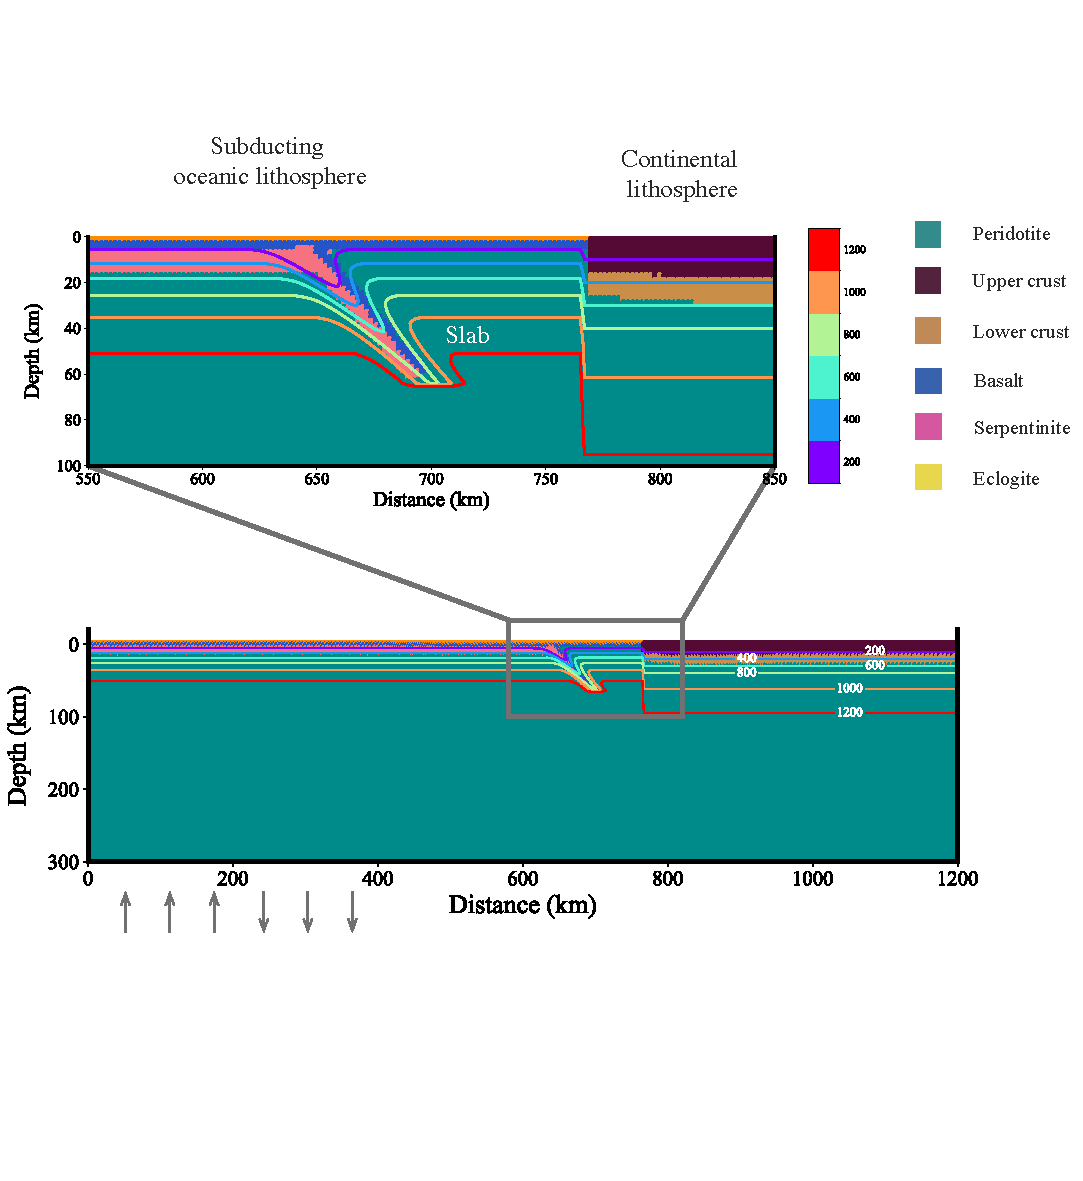
\includegraphics[width=6in]{Ref_Cocos.pdf}
    \caption[墨西哥參考模型設計與邊界條件示意圖]{墨西哥參考模型設計與邊界條件示意圖}
    \label{fig::reference Cocos model}
\end{figure*}

海洋岩石圈年齡為15個百萬年(\citealp{Manea2011Thermal}; \citealp{muller2019}),極為年輕,包含2公里厚的沉積物與6公里厚的玄武岩。由於從地球物理觀測資料得知科克斯板塊隱沒帶富含有大量水份,因此初始模型預設有10公里厚的綠泥岩,並且在隱沒過程中會產生30公里厚的蛇紋岩化橄欖岩。
海洋岩石圈熱構造由第二章式\ref{eq:Half Space Model}提及的半空間冷卻模型決定。
大陸岩石圈包含20公里厚的上部地殼(upper crust)與10公里厚的下部地殼(lower crust),過去有不少研究討論墨西哥區域的熱構造,包含穩態模擬、地磁逆推獲得居禮溫度面與熱流資料研究。本研究主要參考\citealp{Manea2011Curie}所模擬出的岩石圈熱構造,他們結合地磁逆推與隱沒帶模型模擬,推斷在40公里以上地殼地溫梯度每公里攝氏20$^{\circ}$,40公里以下地溫梯度每公里6度,至岩石圈底部為攝氏1330$^{\circ}$。模型頂部邊界溫度為攝氏10$^{\circ}$,底部邊界溫度為攝氏1330$^{\circ}$。
模型左邊界以每年7公分速率往右移動,右邊界則固定不動。
本研究參考的速度同樣來自於\citealp{o2005uncertainties},與智利參考模型相同,模型上邊界為自由表面,而下邊界則為開放邊界,物質可自由進出。

本參考模型的岩石物理特性與智利參考模型類似,除了地函橄欖岩之外有較低的活化能之外,其餘物理性直接相同。
地函橄欖岩活化能的減少造成岩石強度比原先降低10$\%$左右。


\subsection{模型結果}\label{墨西哥參考模型結果}
墨西哥參考模型產生一深度約35-40公里、長度約80-100公里的平坦段。

在隱沒初始時期,由於海洋岩石圈極為年輕,此時海洋岩石圈等深度下溫度遠高於大陸岩石圈,因此模型早期玄武岩相變位置不斷往地函深處移動,於模型5 Myr時來到接近100公里深,如圖\ref{fig::Ref Cocos 26}a。
儘管如此,大陸岩石圈厚度約為100公里,相比於普通大陸岩石圈厚度較薄、溫度較高。
地函楔中橄欖岩融點因大量自由水加入而降低,在距離海溝100公里處發生部分熔融,如圖\ref{fig::Ref Cocos 26}c中黃色線段處。
同時劇烈的脫水作用導致大量蛇紋岩化的橄欖岩在地函楔形成大範圍的低黏滯度區,如圖\ref{fig::Ref Cocos 26}b,促使地函流流動,增加地函楔溫度。
在近地表,海洋地殼上的沉積物、因變形而破碎的海洋地殼與蛇紋岩化橄欖岩在弧前區域堆積。
此時隱沒板塊以一相對高角度的狀態隱沒,角度可達50度,與正常的隱沒帶無異,隱沒角度隨時間變化如圖\ref{fig::Cocos Ref time}c。

在模型進行約略8 Myr時,隱沒板塊在深度30公里左右觸碰大陸岩石圈,隨後隱沒板塊角度開始快速下降,與動水壓力力矩顯著上升的時間點不謀而合,如圖\ref{fig::Cocos Ref time}d。
從圖\ref{fig::Ref Cocos 51}d模型動態壓力可見於地函楔頂部出現一低壓區,其與隱沒板塊下方因板塊彎曲所形成的高壓帶造成明顯的壓力梯度,因此造成動水壓力力矩增加。
同時間圖\ref{fig::Ref Cocos 51}c顯示在地函楔較深處持續發生部分熔融,在地表絕對座標700公里處有火山島弧生成。

隨後從10-15 Myr隱沒傾角逐漸降低,至接近15 Myr時模型達到平坦隱沒條件。
此時,地表上增積岩體累積厚大的沉積物,其所形成的弧前隆起高過火山島弧。
在隱沒板塊上方
這段時間隱沒板塊狀態直接影響岩漿作用特徵。
部分熔融比例幾乎呈指數減少,熔融量在平坦隱沒發育後趨近於0,暗示著火山活動停止,可見圖\ref{fig::Cocos Ref melting time}。
此外,部分熔融發生位置在5百萬年間往內陸移動超過50公里,暗示著地函楔攝氏60$^{\circ}$等溫線逐漸往內陸移動。

隨著隱沒持續進行,穩定的平坦隱沒於20 Myr後不再有明顯幾何上的改變,平坦深度維持在莫合面之下,符合墨西哥區域的接收函數結果(\citealp{PerezCampos2008}),見圖\ref{fig::Ref Cocos 101}a、圖\ref{fig::Ref Cocos 126}a與圖\ref{fig::Ref Cocos 150}a。
隱沒地殼與大陸地殼交界處有一厚度約5公里的沉積物厚層,中間夾雜些許蛇紋岩化橄欖岩,這暗示著隱沒板塊平坦段雖然有長達100公里與大陸地殼接觸,然而交界處物質強度極弱,黏滯度低,很可能無法累積大量應力。
\citealp{Song2009}、\citealp{Song2012SC}利用地震學研究,皆有觀測得平坦段上的交界層為低速層。
\citealp{Song2012SC}更藉由非均相性認為其為經歷強烈剪切的變質岩成分。
\citealp{Manea2017}則認為該弱耦合物質為殘餘的蛇紋岩。
在本參考模型中,獲得的低強度層應為沉積物主導、具有少部分蛇紋岩的岩石成分。

值得一提的是,模型時間30 Myr的壓力剖面\ref{fig::Ref Cocos 150}顯示在大陸岩石圈進地表雖然有火山島弧,然而並沒有顯著的高壓區域,為另一弱偶和特徵的展現。
反觀於智利參考模型中壓力剖面自平坦隱沒發育後(\ref{fig::Nazca_Ref_76}d至\ref{fig::Nazca_Ref_126}d)便在上覆地殼近地表出現長達150公里的高壓區,顯示平坦隱沒於智利參考模型扮演著強耦合的角色。



\begin{figure*}[htp]
    \centering
    \includegraphics[width=6in]{Cocos_a0646frame_26_snapshot_5field_150_v1.pdf}
    \caption[墨西哥參考模型於5 Myr時之結果]{墨西哥參考模型於5 Myr時之結果。}
    \label{fig::Ref Cocos 26}
\end{figure*}

\begin{figure*}[htp]
    \centering
    \includegraphics[width=6in]{Cocos_a0646frame_51_snapshot_5field_150_v1.pdf}
    \caption[墨西哥參考模型於10 Myr時之結果]{墨西哥參考模型於10 Myr時之結果。}
    \label{fig::Ref Cocos 51}
\end{figure*}

\begin{figure*}[htp]
    \centering
    \includegraphics[width=6in]{Cocos_a0646frame_76_snapshot_5field_150_v1.pdf}
    \caption[墨西哥參考模型於15 Myr時之結果]{墨西哥參考模型於15 Myr時之結果。}
    \label{fig::Ref Cocos 76}
\end{figure*}

\begin{figure*}[htp]
    \centering
    \includegraphics[width=6in]{Cocos_a0646frame_101_snapshot_5field_150_v1.pdf}
    \caption[墨西哥參考模型於20 Myr時之結果]{墨西哥參考模型於20 Myr時之結果。}
    \label{fig::Ref Cocos 101}
\end{figure*}

\begin{figure*}[htp]
    \centering
    \includegraphics[width=6in]{Cocos_a0646frame_126_snapshot_5field_150_v1.pdf}
    \caption[墨西哥參考模型於25 Myr時之結果]{墨西哥參考模型於25 Myr時之結果。}
    \label{fig::Ref Cocos 126}
\end{figure*}

\begin{figure*}[htp]
    \centering
    \includegraphics[width=6in]{Cocos_a0646frame_150_snapshot_5field_150_v1.pdf}
    \caption[墨西哥參考模型於30 Myr時之結果]{墨西哥參考模型於30 Myr時之結果。}
    \label{fig::Ref Cocos 150}
\end{figure*}

\newpage
\subsection{墨西哥參考模型脫水位置與岩漿作用}
模型中發生部分熔融與海溝之距離隨時間變化如圖\ref{fig::Cocos Ref melting time}a所示。部分熔融量隨時間變化如圖\ref{fig::Cocos Ref melting time}b。模型中共可分成三段岩漿活躍時期與一段岩漿靜止期。

第一段岩漿活躍期在0-8 Myr隱沒早期,此時熔融量不多,以地函楔中的橄欖岩為主,主要發生在距海溝100公里處,為標準的島弧岩漿特徵。
第二段岩漿活躍期出現在8-20 Myr,由於平坦隱沒在8 Myr開始發育,因此當隱沒板塊發生幾何形狀改變後,部分熔融位置開始往內陸移動,從8-15 Myr之間共移動百餘公里。
岩漿靜止期始於平坦隱沒順利成形的15 Myr,此時因隱沒板塊逐漸貼近大陸地殼下方,莫合面下的地函楔範圍逐漸縮小,因此發生部分熔融的位置不變,但比例逐漸下降,熔融量趨近於0,最終地函楔橄欖岩部分熔融比例於模型進行20 Myr時達到最小值。
\begin{figure*}[h]
    \centering
    \includegraphics[width=5in]{Ref_Cocos_melting_time_v1.pdf}
    \caption[墨西哥參考模型岩漿作用隨時間變化]{墨西哥參考模型岩漿作用隨時間變化,灰色底標出平坦隱沒發育後時間段。(a)部分熔融與海溝之距離隨時間變化圖,縱軸中每個點代表每次部分熔融發生位置,顏色為指數上的部分熔融比例。(b)岩石熔融量隨時間變化圖,熔融量單位為每單位海溝產生之立方公里量中每20萬年瞬時量。顏色代表不同岩相。}
    \label{fig::Cocos Ref melting time}
\end{figure*}

隨後模型進入第三段岩漿活躍期,在20 Myr前,部分熔融狀態有一不連續間隔,熔融位置改變、比例稍微上升,如圖\ref{fig::Cocos Ref melting time}a。
這暗示著岩漿作用區域改變,並且在該不連續時間段段後,部分熔融又重新以緩慢的速率往內陸遷移,與平坦隱沒平坦段的持續發育增長有關,隱沒板塊平坦段長度隨時間變化見圖\ref{fig::Cocos Ref time}a。
平坦隱沒具有與正常隱沒帶不同的溫壓路徑,由於其地殼在等深度下維持不變長達近80公里,在整段平坦段中壓力不變,但越靠內陸側之岩石溫度越高,此時鐵鎂岩相與沉積岩相很有可能會通過固熔點,導致海洋地殼發生部分熔融。
圖\ref{fig::Cocos Ref melting time}所統計之熔融岩相量顯示在20 Myr後陸續發生沉積物部分熔融,甚至在23 Myr後橄欖岩熔融消失,此特徵與該地區的岩漿觀測研究相符。

本參考模型的岩漿庫規模遠大於智利參考模型,累積的岩漿庫體積約是智利參考模型的100倍以上,根本原因為本研究所使用的岩漿庫冷卻參數與溫度高度相關。
在墨西哥模型中,無論海洋岩石圈或大肚岩石圈溫度梯度皆比智利參考模型高,因此岩漿庫不易冷卻,火山活動活躍。

將模型中部分熔融事件與岩漿庫絕對位置繪出,分別獲得圖\ref{fig::Cocos Ref 2Dtime series}a, b。
圖中顯示顯著的三段岩漿活躍期,第一段岩漿活躍期發生在絕對座標500至650公里、距海溝100公里之間,與正常的島弧岩漿活動特徵類似。
第二段岩漿活躍期發生在絕對座標650-750公里內,熔融深度、岩漿庫深度較第一段活躍期深,岩漿量也較大。
最終第三段岩漿活躍期發生在絕對座標750-830公里內,岩漿庫規模皆沒有前兩段活躍期大,但位置較集中,並且持續時間最長。

玄武岩至榴輝岩相變位置見圖\ref{fig::Cocos Ref 2Dtime series}c。
在模型早期,因隱沒岩石圈溫度比大陸岩石圈高,因此玄武岩至榴輝岩相變深度從40公里逐漸往接近100公里移動。
然而從圖\ref{fig::Ref Cocos 26}a與c可見儘管發生相變發生位置逐漸變深,該時期是一高角度隱沒帶,並沒有明顯的隱沒傾角趨緩特徵。
隨後在15 Myr之後,玄武岩相地殼來到模型時間段間最小長度,亦即玄武岩進入海溝後於15 Myr時會以最短的速度相變成榴輝岩相,圖\ref{fig::Cocos Ref time}d中顯示在15 Myr後重力力矩達到最高點,同樣可驗證該時間點為榴輝岩相長度達到模型中最大值,然而此時間剛好發生在平坦隱沒形成後不到一個百萬年。
因此,再次證明玄武岩相變與榴輝岩的出現仍然可以形成長久穩定的平坦隱沒。
隨後由於平坦隱沒地殼往內陸延伸的速度大於隱沒地殼增溫的速度,因此玄武岩相變深度再次往內陸推進。
平坦段中增溫速度緩慢顯示其上方沒有顯著的不可逆變形,因此摩擦熱不大,這進一步意味著平坦段上的應力狀態以低耦合為主,再次與觀測資料吻合(\citealp{moran2007cenozoic}, \citealp{PerezCampos2008})。

\begin{figure*}[ht]
    \centering
    \includegraphics[width=4in]{Cocos_a0646_2Dtime_series_v1.pdf}
    \caption[墨西哥參考模型部分熔融、岩漿庫與玄武岩相變時空關係圖]{墨西哥參考模型部分熔融、岩漿庫與玄武岩相變時空關係圖。}
    \label{fig::Cocos Ref 2Dtime series}
\end{figure*}

\newpage
\subsection{參考模型隱沒板塊與其轉動平衡}
模型中的平坦隱沒長度與深度隨時間變化見圖\ref{ffig::Cocos Ref time}a, b,平坦段深度與長度的定義已於\ref{平坦隱沒定義}節提及。

在平坦隱沒發育初期,模型時間15-20 Myr之間平坦隱沒還在緩慢發育,並且玄武岩相變深度持續加深,因此儘管重力力矩逐漸下降,平坦段長度並沒有顯著增加,隨後於20 Myr後,重力力矩不再變化,平坦段開始增長,至30 Myr可到達超過100公里長。
儘管平坦隱沒段長度逐漸變長,然而模型中平坦隱沒段深度於全時段皆沒有劇烈改變,均落在30-40公里深上下。
平坦隱沒段長度與深度皆與觀測資料吻合。

模型中隱沒板塊於150公里之內的角度變化如圖\ref{fig::Cocos Ref time}c所示。
在模型早期,角度隨時間增加直到5 Myr,隨後隨著動水壓力力矩快速增加(圖\ref{fig::Cocos Ref time}d),隱沒傾角開使緩慢下降。
在模型時間15 Myr後,隱沒傾角不再劇烈改變,暗示平坦隱沒開始發育後,隱沒帶趨近穩定,不再有幾何形狀上的變化。

\begin{figure*}[hb]
    \centering
    \includegraphics[width=4in]{Ref_Cocos_time_v1.pdf}
    \caption[墨西哥參考模型隱沒板塊狀態隨時間變化]{墨西哥參考模型隱沒板塊狀態隨時間變化。}
    \label{fig::Cocos Ref time}
\end{figure*}

模型中不同時間段的重力力矩與動水壓力力矩值如圖\ref{fig::Cocos Ref time}d。
由於本參考模型有玄武岩相變位置改變的現象,因此重力力矩在時間軸上改變劇烈。
模型早期有顯著的玄武岩相變深度變化,然而在隱沒板塊觸碰到大陸地殼後,被動導致隱沒傾角逐漸減少,玄武岩相變深度逐漸回歸至50公里深,隱沒板塊溫度逐漸升高。
重力力矩在模型時間15 Myr達到最大值,隨後隨著平坦隱沒發育,玄武岩相變位置有水平方向上的變化,逐漸往內陸移動,導致重力力矩逐漸減小。

動水壓力力矩增加起始時間早於重力力矩,應發生於隱沒板塊觸碰到大陸地殼的瞬間開始大幅增加。
在平坦隱沒發育後,動水壓力力矩雖有上升趨勢,然而增加斜率緩慢。
導致本模型能維持平坦隱沒持續15 Myr的原因可能有兩種,
第一,因為玄武岩相變深度加深的現象導致重力力矩在15 Myr後持續減少,因此平坦隱沒能穩定存在。
第二,早在動水壓力力矩巨幅增加的時期,便已經決定整個隱沒系統的動態穩定。由於15 Myr後動水壓力力矩依然有極大的轉動力矩,因此無論重力力矩是否下降,平坦隱沒皆可穩定存在。
% !TeX root = ../main.tex

\chapter{討論}

針對兩種平坦隱沒模型,各有不同的觀測資料特徵。
本章將模型結果與觀測資料進行比對,討論兩種平坦隱沒類型所具有的構造特色與岩漿作用狀態。
最後,將討論模型中可能影響平坦隱沒的形成原因。

\section{隱沒系統的耦合狀態}
隱沒板塊的耦合概念在1970年代晚期開始盛行(\citealp{uyeda1979back}; \citealp{ruff1980seismicity}),\citealp{uyeda1979back}以隱沒板塊的年紀將隱沒帶分成兩種類型:第一種是年老隱沒板塊的馬尼亞納型(Mariana type)隱沒帶,第二種是年輕隱沒板塊的智利型(Chilean type)隱沒帶,示意圖如圖\ref{fig::end-member subduction}所示。
\begin{figure*}[htp]
    \centering
    \includegraphics[width=6in]{2020subduction_type.png}
    \caption[隱沒帶的兩種型態示意圖,摘自\citealp{Yan2020}]{隱沒帶的兩種型態示意圖,摘自\citealp{Yan2020}。(a)馬尼亞納型隱沒帶(b)智利型隱沒帶}
    \label{fig::end-member subduction}
\end{figure*}

馬尼亞納型隱沒帶中隱沒板塊年紀較大、密度較大,重力較大造成隱沒板塊垂直分量上的拉力較大、隱沒傾角較高,與上覆板塊的接觸面積相對較小,可見圖\ref{fig::end-member subduction}a。
此類隱沒帶的應力不易累積,容易發生潛移活動,地震事件規模較小且通常為伸張地震,故馬尼亞納型隱沒帶又可稱為弱耦合(weak coupling)隱沒帶。
此外,高角度的隱沒板塊造成地函楔容易發生強烈對流,伴隨隱沒帶的部分熔融作用,在上覆板塊側發生拉張現象,可能會產生弧後張裂(back-arc spreading)(\citealp{lallemand2005relationships})。
反之智利型隱沒帶因隱沒板塊溫度較高、密度較小,故隱沒傾角較低,在聚合板塊交界處產生較大的板塊接觸面積,如圖\ref{fig::end-member subduction}b。
通常此類隱沒帶會容易產生低角度的班尼奧夫帶,地震事件多以逆衝斷層為主,且發生過多起大規模(Mw>8.0)地震事件(\citealp{uyeda1979back})。
上覆板塊側有顯著的壓縮應力(\citealp{hu2021southward}),可能會在弧後出現許多皺褶與斷層,因此智利型隱沒帶亦會被視為強耦合(strong coupling)隱沒帶。

\subsection{智利平坦隱沒的耦合狀態}
過去的研究注意到智利上覆板塊的地殼地震事件數目在平坦隱沒區域較多(\citealp{jordan1983andean}; \citealp{smalley1993basement}),表明平坦隱沒區域具有比正常隱沒帶更強的板塊間耦合。
\citealp{gutscher2002andean}統計智利沿岸在距海溝250-800公里的所有地震事件所釋放之能量總和,以南北向一度以內為單位,獲得板塊釋放的地震能量直方圖(見圖\ref{fig::Chile_seismicity})。
總體而言,智利中部平坦隱沒上方的板塊所釋放出的地震能量比北部玻利維亞段高出5倍,比南段智利高出10倍。
\citealp{jordan1983andean}分析智利沿岸大地震的震源機制解,顯示該區域以壓縮型地震主導,他認為隱沒邊界應力有效傳遞到上覆板塊,並且在平坦隱沒段有更高程度的板塊間耦合。

\begin{figure*}[htp]
    \centering
    \includegraphics[width=5in]{Seismicity and Energy of Andes.png}
    \caption[智利沿岸自21$^\circ$S到44$^\circ$S的上板塊地震活動統計分析,摘自\citealp{gutscher2002andean}]{智利沿岸自20$^\circ$S到40$^\circ$S的上板塊地震活動統計分析,摘自\citealp{gutscher2002andean}。這裡採用深度<70公里的地震事件總能量,單位為10$^6$焦耳。右側數字表示1900-1963年/1964-1995年間所示分的地震能量。數字下灰色底框標示出平坦隱沒段的位置。
    }
    \label{fig::Chile_seismicity}
\end{figure*}

本研究智利參考模型的水平應力(Sxx)剖面圖如圖\ref{fig::Sxx_and_Pressure_Chile}a所示。
其中,水平應力大於0表示拉張,水平應力小於0表示壓縮。
上覆板塊側的水平應力在平坦隱沒段上地殼處有較小值,表示壓縮應力的存在。
上覆板塊的壓縮應力在水平方向上可分為兩區域,第一個區域位在近地表30公里以上、絕對座標550-650公里之間,其下方對應到隱沒板塊上凹變形處位置。
第二個區域較不明顯,位於絕對座標750-800公里、深度50-70公里處,對應到隱沒板塊下傾位置。
動水壓力剖面同樣可以觀察到類似的現象,在圖\ref{fig::Sxx_and_Pressure_Chile}b中,上覆板塊淺層於絕對座標550-650公里處有很大的正壓力,與圖\ref{fig::Sxx_and_Pressure_Chile}a中的壓縮應力位置相似。

\begin{figure*}[h]
    \centering
    \includegraphics[width=5.5in]{Sxx_and_Pressure_Chile_of_201.pdf}
    \caption[智利參考模型於40 Myr的水平軸差應力與動水壓力剖面]{智利參考模型於40 Myr的水平軸差應力與動水壓力剖面,其中應力正向代表拉張應力,負向代表壓縮應力。}
    \label{fig::Sxx_and_Pressure_Chile}
\end{figure*}
\subsection{墨西哥平坦隱沒的耦合狀態}
儘管如此,墨西哥平坦隱沒並沒有強耦合的特徵。
\citealp{PerezCampos2008}的接收函數結果顯示墨西哥的隱沒板塊平坦段深度直接位於莫荷面下方,因此隱沒板塊與上覆板塊的接觸面材質為海洋地殼與下部大陸地殼的成分,幾乎不包含任何大陸地函軟流圈(continental mantle asthenosphere),此時板塊介面在聚合過程中理論上應產生很大的摩擦力。
此外,墨西哥隱沒帶被視為侵蝕型隱沒(subduction erosion)(\citealp{stern2011subduction}),其證據包含現今外海的沉積物厚度約200公尺(\citealp{manea2003sediment}),並且擁有快速的聚合速率(\citealp{o2005uncertainties})。
再配合年輕隱沒帶的低傾角隱沒特徵,墨西哥平坦段聚合板塊接觸面積極大。
種種物理跡象表明該區域應該為強耦合環境。
然而墨西哥平坦隱沒段的地震活動度極低,格雷羅無震帶(\citealp{kostoglodov2003large})便位於平坦段上,表明平坦段並非處於強耦合狀態。
除此之外,平坦隱沒上方並沒有顯著的水平壓縮現象(\citealp{nieto2006latest}; \citealp{moran2007cenozoic},這與強耦合的特徵互相矛盾。
對此,\citealp{Manea2011Thermal}模擬墨西哥平坦隱沒剖面的熱構造。
隱沒板塊段上海洋地殼與沉積物絕大部分在距海溝250公里前便完成脫水,大量的水分可能釋放進入下大陸地殼中,導致岩石強度降低,不容易累積大量應力。
該地區的非火山微震(non volcanic tremor)發生位置與海洋地殼的脫水位置相吻合\citealp{Manea2011Thermal},慢地震(slow slip event)事件位置則與沉積物的脫水位置吻合\citealp{Song2009}。
大量的微震與慢地震事件暗示著該區域為弱耦合隱沒帶。

本研究墨西哥參考模型的水平應力(Sxx)剖面圖如圖\ref{fig::Sxx_and_Pressure_Mexico}a所示。
上覆板塊側的水平應力在上部地殼與下部地殼底部各有一層高區。
此外,在絕對座標700公里與800公里處的火山島弧下方也具有地區性的水平應力小值,其為火山形成的荷重所造成。
與智利參考模型相比,墨西哥參考模型的上覆版塊沒有顯著的壓縮應力存在。
動水壓力剖面同樣可以觀察到類似的現象,如圖\ref{fig::Sxx_and_Pressure_Mexico}b所示,上覆板塊側除了上下地殼交界處與莫荷面處有較高的正壓力外,並沒有顯著來自隱沒板塊介面所提供的正壓力。
\begin{figure*}[ht!]
    \centering
    \includegraphics[width=5in]{Sxx_and_Pressure_Phase_Mexico_of_201_v5.pdf}
    \caption[墨西哥參考模型中於40 Myr的剖面]{墨西哥參考模型中於40 Myr的水平軸差應力、動水壓力與岩相剖面。(a)水平軸差應力剖面,其中應力正向代表拉張應力,負向代表壓縮應力。(b)動水壓力剖面。(c)模型岩相剖面,岩相顏色請見圖\ref{fig::Ref Cocos 26}。}
    \label{fig::Sxx_and_Pressure_Mexico}
\end{figure*}

本研究於第\ref{墨西哥隱沒帶地球物理觀測}節與第\ref{墨西哥參考模型結果}節皆有提及地震學研究在墨西哥平坦隱沒區域的板塊介面中發現一層低速層(\citealp{PerezCampos2008}),\citealp{Song2009}估計該低速層厚度約3-5公里且V$_S$速度約每秒2-2.7公里,大約降低26-40$\%$左右。
過去對於該低速層的成分有諸多解釋,\citealp{Song2012SC}認為其為經歷強烈剪切的變質岩成分。
\citealp{Manea2017}則認為該弱耦合物質為殘餘的蛇紋岩。

從墨西哥參考模型的岩相圖\ref{fig::Sxx_and_Pressure_Mexico}c可見隱沒板塊與大陸地殼的介面中具有厚度4-8公里、以沉積岩為主參雜少許蛇紋岩化橄欖岩的弱物質。
由於該弱物質層的岩石強度極弱,故隱沒板塊介面成為弱耦合介面,上覆板塊的壓縮應力較小。
因此,並非所有低傾角隱沒帶皆具有強耦合的特徵。

\section{平坦隱沒中的埃達克岩}\label{平坦隱沒中的埃達克岩}
埃達克岩(adakite)最初由\citealp{kay1978aleutian}觀測阿留申群島中Adak Island上一種高La/Yb、高Sr/Y以及富含大離子半徑元素(large ion lithophile (LIL)- element-rich)的安山岩,其特徵與一般的火山島弧安山岩不相同,爾後\citealp{defant1990derivation}將其命名為埃達克岩。
由於埃達克岩具有特殊的全岩地球化學性質,一般多半利用Sr/Y-Y作圖與(La/Yb)$_N$-Yb$_N$作圖區別埃達克岩與一般的島弧中酸性安山岩,如圖\ref{fig::AdakiteY}。

\begin{figure*}[h]
    \centering
    \includegraphics[width=5in]{AdakiteY.jpg}
    \caption[Sr/Y-Y作圖與(La/Yb)$_N$-Yb$_N$作圖]{(A)Sr/Y-Y作圖與(B)(La/Yb)$_N$-Yb$_N$作圖,摘自\citealp{castillo2012adakite}。通常用於區分埃達克岩與普通島弧安山岩、石英岩與流紋岩(normal arc andesite, dacite and rhyolite, ADR)。紫色實線邊界來自於\citealp{richards2007special}所提出菲律賓中南部埃達克岩與普通島弧安山岩的資料。}
    \label{fig::AdakiteY}
\end{figure*}

早期認為埃達克岩是年輕的(< 7 Ma)隱沒海洋玄武岩發生部分熔融產生的中酸性火山岩(\citealp{defant1990derivation}; \citealp{peacock1994partial})。
由於埃達克岩的定義來自岩石化學組成分定量分析,隨著相關研究累積,顯示高壓變質基性岩的部分熔融皆具有埃達克岩的特徵,
因此埃達克岩性質的火成岩可已在多種不同地體環境下產生(\citealp{martin2005overview}),以下列出最常見的四種:

(1)隱沒海洋地殼的熔融(\citealp{defant1990derivation}),隨後埃達克岩中的低Nd、高Sr同位素特徵被認為是隱沒海洋沉積物參與部分熔融所產生(\citealp{stern1996role}; \citealp{gomez2003temporal}),又有人稱其為high-SiO$_2$ adakites (\citealp{martin2005overview})。

(2)增厚大陸下地殼底部的基性岩熔融(\citealp{kay1996magmatic})。
在高壓環境下,基性岩密度過高時無法穩定存在於大陸地殼底部,因此部分熔融產生。
通常需要長時間的地殼增厚(\citealp{kay2002magmatism})才會形成高壓下的高密度基性岩,因此這種形成機制比較可能會發生在島弧岩漿作用事件中末期。

(3)普通島弧安山岩受地殼成分污染,導致岩漿混合,其稱為low-SiO$_2$ adakites (\citealp{martin2005overview}),與(1)成因中的high-SiO$_2$ adakites相對。
此埃達克岩具有較高的地函組成相關元素(MgO、K、Nb、Cr、Ni等)。

(4)來自一般的島弧基性岩漿於高壓(> 12 kbar)環境下,以石榴子石為主的結晶分化產物(\citealp{moyen2009high}),例如菲律賓蘇里高半島的埃達克岩。

一般來說,上述成因中,只有(1)與(2)兩種成因可被稱為埃達克岩,而(3)與(4)所產生之高Sr/Y類似因物質交換而繼承埃達克岩特徵,稱作類埃達克岩(Adakite-like rocks)(\citealp{kay2002magmatism}; \citealp{goss2013andean})。

早期在南美洲的平坦隱沒區域發現部分埃達克岩的紀錄,\citealp{Gutscher2000Bcan}為此提出一概念模型,為平坦隱沒特殊的溫壓條件所生成埃達克岩。
如同\ref{墨西哥參考模型脫水位置與岩漿作用}節所提及,平坦隱沒具有與正常隱沒帶不同的溫壓路徑,如圖\ref{fig::Flat slab PT}中所繪,此時鐵鎂岩相與沉積岩相很有可能會通過固熔點,導致海洋地殼發生部分熔融。

\begin{figure*}[ht!]
    \centering
    \includegraphics[width=4in]{Flat slab PT.png}
    \caption[隱沒板塊頂部可能的溫壓路徑圖,摘自\citealp{Gutscher2000Bcan}]{隱沒板塊頂部可能的溫壓路徑圖,摘自\citealp{Gutscher2000Bcan}。Ec—榴輝岩(eclogite),Am—角閃岩(amphibolite),Ga—石榴石(garnet),Hb—角閃石(hornblende)。
    圓形為正常隱沒帶中的溫壓路徑,菱形與正方形則為平坦隱沒的溫壓路徑。其中,灰色底部分為隱沒板塊可能的部分熔融區。
    }
    \label{fig::Flat slab PT}
\end{figure*}

\subsection{墨西哥平坦隱沒的岩漿作用}
在墨西哥,地球化學上所認定的埃達克岩的特徵之一為高Gd/Yb與高SiO$_2$,如圖\ref{fig::Cocos_geochemisty}b與圖\ref{fig::Cocos_geochemisty}c所示。
跨墨西哥火山帶最初於早中新世(約19 Ma)開始噴發,主要為亞鹼性(sub-alkaline)岩石,由安山岩和英安岩組成,隨著火成岩噴發位置離海溝越來越遠,地球化學特徵表明越往北(遠離海溝)的火成岩,隱沒帶中的流體量越少(\citealp{ferrari2012dynamic})。
這個趨勢在15 Ma左右被侵入的埃達克岩中斷(\citealp{mori2007effects}),見圖\ref{fig::Cocos_geochemisty}a紅色與藍色點,值得注意的是,具有埃達克岩特徵的樣本幾乎都與海溝距離超過400公里。
目前學界一致認同墨西哥平坦隱沒區域所發現的埃達克岩樣本皆為隱沒海洋地殼與沉積物的產物(\citealp{Gutscher2000Bcan}; \citealp{ferrari2012dynamic}; \citealp{Manea2017})。

\begin{figure*}[ht!]
    \centering
    \includegraphics[width=5in]{Cocos_Volcano_v2.pdf}
    \caption[墨西哥區域火山島弧地球化學分析,摘自\citealp{ferrari2012dynamic}]{墨西哥區域火山島弧地球化學分析,摘自\citealp{ferrari2012dynamic}。白點為距現今火山弧前緣小於150公里的樣本,藍色點為具現今火山弧前緣大於150公里且位在西經99-101$^{\circ}$的樣本,紅色點為具現今火山弧前緣小於150公里且位在西經96.4-99$^{\circ}$的樣本。(a)火成岩樣本年紀與現今海溝距離作圖。(b)火成岩樣本中的SiO$_2$含量與現今海溝距離作圖。(c)火成岩樣本中Gd/Yb比值與現今海溝距離作圖。(d)墨西哥中新世火山位置圖。細虛線表示到海溝的距離,粗虛線是\ref{平坦隱沒中的埃達克岩}圖例中使用的邊界。 CC: Cerro Colorado dome,CG: Cerro Grande volcan塞羅格蘭德火山, LJ: La Joya volcan拉霍亞火山, PH: Palo Huérfano 火山, PS: Palma Sola帕爾馬索拉,SA: Sierra de Angangueo塞拉利昂德安甘格奧, SM: San Martín聖馬丁, SMC: Sierra de Mil Cumbres, T-M: Tenancingo–Malinalco特南寧哥-馬利納爾科, Za: Zamorano volcano薩莫拉諾火山, Zi: Zimapán area Zimapán 地區。
    }
    \label{fig::Cocos_geochemisty}
\end{figure*}

在墨西哥參考模型中,確實有海洋地殼部分熔融的現象。
圖\ref{fig::Cocos Ref melting time}b、c中顯示平坦隱沒形成、於模型時間15 Myr前後開始發生榴輝岩的部分熔融。
榴輝岩的部分熔融比例在平坦隱沒形成初期快速增加,在15-20 Myr之間可達50-70$\%$。
在20 Myr後,榴輝岩的部分熔融比例維持5-20$\%$之間,在時間軸上沒有太大改變。
然而沉積物自23 Myr後便成為墨西哥參考模型熔融源的主導岩石。
儘管多數研究已證實隱沒沉積物大量熔融的存在(\citealp{van2011subduction}; \citealp{Forster2021}),本研究認為該結果需要進一步確認。
本研究中,所選用的沉積物固相線為飽和水固相線(\citealp{van2011subduction}),然而模型中並沒有考量各岩石的含水量多寡,因此部分熔融的形成機制需要更多考量。

\citealp{stern1996role}針對埃達克岩樣本進行分析,表示埃達克岩中約有35-90$\%$的隱沒板塊質量,包含玄武岩、榴輝岩與沉積物。
圖\ref{fig::melting_eclogite_ratio}是墨西哥參考模型在時間軸上岩漿熔融源與熔融量變化圖,只關注於平坦隱沒發生後的岩石熔融。
圖\ref{fig::melting_eclogite_ratio}b顯示模型中榴輝岩的熔融比例與岩漿庫體積,在平坦隱沒剛形成時(15-20 Myr),所有熔融岩中,有超過40$\%$為榴輝岩,爾後榴輝岩體積比例維持10-20$\%$。
由於本研究並沒有考慮大陸地殼中的岩漿作用,以及岩漿內物質置換、結晶分異作用與岩石含水量對岩漿庫的影響,因此無法充分說明模型中所產生的火山島弧是否確切為埃達克岩的成分。
然而從模型中岩漿作用熔融源分析可證明(見圖\ref{fig::melting_eclogite_ratio}a),隱沒板塊物質確實可以發生熔融。

圖\ref{fig::Mexico_arc_location}顯示墨西哥參考模型中地表出現兩處的火山島弧。
第一處的火山島弧出現於距海溝130-180公里處,可以對應至圖\ref{fig::Cocos Ref 2Dtime series}b中的第二區岩漿庫(Magma Chamber 2)。
第二處的火山島弧出現於距海溝260-280公里處,可以對應至圖\ref{fig::Cocos Ref 2Dtime series}b中的第三區岩漿庫(Magma Chamber 3)。
本研究所產生的火山島弧與海溝距離不及圖\ref{fig::Cocos_geochemisty}中的墨西哥火山島弧,不過確實可獲得沿海溝距離上火成岩成分的劇烈變化結果。

\begin{figure*}[ht!]
    \centering
    \includegraphics[width=6in]{slab_melting.pdf}
    \caption[墨西哥參考模型部分熔融源岩與岩漿庫分析]{墨西哥參考模型部分熔融源岩與岩漿庫分析。(a)同圖\ref{fig::Cocos Ref melting time}b,聚焦在13-40 Myr時期的部分熔融源岩,熔融量單位為每單位海溝產生之立方公里量中每20萬年瞬時量,模型中包含橄欖岩(綠色)、沉積岩(橘色)與榴輝岩(深藍色)熔融。灰底為平坦隱沒發生時間。(b)黃底柱狀為岩漿庫體積,藍點為榴輝岩瞬時熔融體積佔整體瞬時熔融體積的比例。
    }
    \label{fig::melting_eclogite_ratio}
\end{figure*}

\begin{figure*}[ht!]
    \centering
    \includegraphics[width= 5in]{Mexico_arc_location_v1.pdf}
    \caption[墨西哥參考模型火山島弧與海溝距離隨時間變化]{墨西哥參考模型火山島弧與海溝距離隨時間變化。其中咖啡色為熔融源岩以橄欖岩為主的火山島弧,藍色則為熔融源岩以沉積物與榴輝岩為主的火山島弧。
    }
    \label{fig::Mexico_arc_location}
\end{figure*}

\newpage
\subsection{智利平坦隱沒的岩漿作用}

\citealp{Gutscher2000Bcan}認為南美洲平坦隱沒區域所出露的埃達克岩為隱沒板塊熔融的產物,在他們的研究中僅使用概念模型解釋埃達克岩成因,然而\citealp{kay2002magmatism}近一步對埃達克岩樣本進行地球化學分析,他們認為智利區域的埃達克岩為上述成因中的第(3)種,埃達克岩漿來自於普通島弧安山岩漿與地殼熔融發生岩漿混合,是為low-SiO$_2$ adakites。
由於本研究並沒有考慮大陸地殼成分岩石發生部分熔融,因此無法從參考模型中獲得\citealp{kay2002magmatism}所認為的結果。
然而,將智利參考模型隱沒地殼頂部溫壓狀態與隱沒板塊相圖比較(見圖\ref{fig::chile_slab_PT}),隱沒板塊並沒有通過隱沒板塊含水固相線。
此外,智利參考模型的平坦深度在100公里左右,圖\ref{fig::chile_slab_PT}中壓力維持不變且溫度持續增加的範圍落在3 GPa與攝氏500-800 $^{\circ}$之間,圖\ref{fig::Flat slab PT}中\citealp{Gutscher2000Bcan}的概念模型平坦段範圍落在2.5 GPa與攝氏400-900$^{\circ}$,兩者有顯著差異。
以智利平坦隱沒區的平坦段深度100公里來看,智利參考模型的結果較接近真實情形。
這說明本研究可以藉由排除\citealp{Gutscher2000Bcan}中所認為的埃達克岩形成方式。

\begin{figure*}[ht!]
    \centering
    \includegraphics[width=4in]{chile_slab_PT_v1.pdf}
    \caption[智利參考模型隱沒地殼頂部於40 Myr的溫壓圖]{智利參考模型隱沒地殼頂部於40 Myr的溫壓圖。其中綠線為本研究中玄武岩至榴輝岩的相變條件,橘色線為含水固相線。綠色點為隱沒地殼頂部每2-5公里的溫壓狀態。
    }
    \label{fig::chile_slab_PT}
\end{figure*}

\newpage
\section{為什麼會形成平坦隱沒}
由於平坦隱沒的形成原因至今依然是一開放性問題,以下將討論隱沒帶中不同構造區對隱沒系統的影響,以及本研究模型中產生平坦隱沒的可能關鍵原因。
本節測試一系列數值模型參數,模型參數表見表\ref{模型參數列表}。

\begin{table}[htp]\large
    \caption[模型參數列表]{模型中參數列表}
    \label{模型參數列表}
    \renewcommand{\arraystretch}{1.2}
    \centering
    \begin{tabular}{|lllll|}
        \hline
        \multicolumn{5}{|c|}{a Upper Plate Thickness}                                                 \\ \hline
        model        & P$_0$                   & $\lambda_0$             & thickness & serpentinite \\ \hline
        Nazca\_a01 & 4.5 $\times$ 10$^{-15}$ & 1.6 $\times$ 10$^{-12}$ & 120       & 5            \\
        Ref\_Nazca   & 4.5 $\times$ 10$^{-15}$ & 1.6 $\times$ 10$^{-12}$ & 130       & 5            \\
        Nazca\_a02 & 4.5 $\times$ 10$^{-15}$ & 1.6 $\times$ 10$^{-12}$ & 140       & 5            \\
        Nazca\_a03 & 4.5 $\times$ 10$^{-15}$ & 1.6 $\times$ 10$^{-12}$ & 150       & 5            \\
        Nazca\_a04 & 4.5 $\times$ 10$^{-15}$ & 1.6 $\times$ 10$^{-12}$ & 160       & 5            \\ \hline
        \multicolumn{5}{|c|}{Serpentinite Thickness}                                                \\ \hline
        model        & P$_0$                   & $\lambda_0$             & thickness & serpentinite \\ \hline
        Nazca\_b01 & 4.5 $\times$ 10$^{-15}$ & 1.6 $\times$ 10$^{-12}$ & 130       & 2.5          \\
        Ref\_Nazca   & 4.5$\times$ 10$^{-15}$  & 1.6 $\times$ 10$^{-12}$ & 130       & 5            \\
        Nazca\_b02 & 4.5 $\times$ 10$^{-15}$ & 1.6 $\times$ 10$^{-12}$ & 130       & 7.5          \\
        Nazca\_b03 & 4.5 $\times$ 10$^{-15}$ & 1.6 $\times$ 10$^{-12}$ & 130       & 10           \\
        Nazca\_b04 & 4.5 $\times$ 10$^{-15}$ & 1.6 $\times$ 10$^{-12}$ & 130       & 15           \\ \hline
        \multicolumn{5}{|c|}{Magma Parameters}                                                      \\ \hline
        model        & P$_0$                   & $\lambda_0$             & thickness & serpentinite \\ \hline
        Ref\_Nazca   & 4.5 $\times$ 10$^{-15}$ & 1.6 $\times$ 10$^{-12}$ & 130       & 5            \\
        Nazca\_c01 & 4.5 $\times$ 10$^{-14}$ & 1.6 $\times$ 10$^{-12}$ & 130       & 5            \\
        Nazca\_c02 & 4.5 $\times$ 10$^{-13}$ & 1.6 $\times$ 10$^{-12}$ & 130       & 5            \\
        Nazca\_c03 & 4.5 $\times$ 10$^{-15}$ & 1.6 $\times$ 10$^{-13}$ & 130       & 5            \\
        Nazca\_c04 & 4.5 $\times$ 10$^{-14}$ & 1.6 $\times$ 10$^{-13}$ & 130       & 5            \\
        Nazca\_c05 & 4.5 $\times$ 10$^{-13}$ & 1.6 $\times$ 10$^{-13}$ & 130       & 5            \\
        Nazca\_c06 & 4.5 $\times$ 10$^{-15}$ & 1.6 $\times$ 10$^{-14}$ & 130       & 5            \\
        Nazca\_c07 & 4.5 $\times$ 10$^{-14}$ & 1.6 $\times$ 10$^{-14}$ & 130       & 5            \\
        Nazca\_c08 & 4.5 $\times$ 10$^{-13}$ & 1.6 $\times$ 10$^{-14}$ & 130       & 5            \\
        Nazca\_c09 & 4.5 $\times$ 10$^{-15}$ & 1.6 $\times$ 10$^{-15}$ & 130       & 5            \\
        Nazca\_c10 & 4.5 $\times$ 10$^{-14}$ & 1.6 $\times$ 10$^{-15}$ & 130       & 5            \\
        Nazca\_c11 & 4.5 $\times$ 10$^{-13}$ & 1.6 $\times$ 10$^{-15}$ & 130       & 5            \\ \hline
    \end{tabular}
\end{table}

\subsection{均質的隱沒板塊}
本研究的兩種參考模型中,隱沒板塊上皆不存在任何非均質(heterogeneous)構造或任何例外的物理特性。
同\ref{平坦隱沒的數值模型}所述,過去的數值模型提出許多降低隱沒系統重力力矩的可能原因,包含加入一段不會發生玄武岩相變的海洋地殼(\citealp{Liu2016}; \citealp{Gerya2009})、延後榴輝岩相的相變時間(\citealp{van2002role})、增厚隱沒海洋地殼(\citealp{Liu2016}; \citealp{axen2018basal})、降低整體隱沒岩石圈密度(\citealp{Gerya2009})以及設計隱沒板塊隱沒後斷裂(\citealp{Liu2016}; \citealp{axen2018basal})等。

早期研究認為隱沒的海洋高原最有可能是平坦隱沒的形成原因(\citealp{gutscher2002andean})。
\citealp{Skinner2013}利用磁力條帶重建納茲卡板塊上海洋高原及洋脊位置,並且計算其隱沒進入南美板塊的時間。
他們的研究表明隱沒的地殼增厚體與平坦隱沒發生時間錯開,因此平坦隱沒的形成原因可能無法完美的被地殼增厚體所解釋。
\citealp{Marot2014}利用表面波地震層析成像探討智利平坦隱沒下方的速度構造,他們的結果沒有看到任何異常的隱沒地殼,並支持納茲卡板塊在速度上與厚度上皆是均勻的構造。
放眼至地球上其他區域,許多區域皆有海脊隱沒的證據,例如勘察加半島(Kamchatka)有皇帝海脊(Emperor Ridge)隱沒、琉球(Ryukyu)有大東海脊(Daito Ridge)隱沒以及馬里亞納(Mariana)與馬庫斯—內克海脊(Marcus-Necker Ridge)隱沒,然而只有秘魯與智利有平坦隱沒的特徵。
另一個問題是,在墨西哥有平坦隱沒的特徵,然而墨西哥沒有任何海脊或海洋高原的隱沒紀錄,因此增厚的海洋地殼發生平坦隱沒的理論近年來逐漸站不住腳(\citealp{schellart2020control}; \citealp{Schellart2021})。

\subsection{上覆板塊的溫度構造}
過去對於平坦隱沒上覆板塊溫度構造的研究並不多。
\citealp{Thermal2012}的數值模型討論上覆板塊的溫度構造與平坦隱沒的關係,該研究中,上覆板塊與隱沒板塊皆使用平板冷卻模型(plate cooling model),固定板塊底部的溫度為攝氏1450$^\circ$且板塊厚度為95公里。
他們結果表示較冷硬的上覆板塊較容易產生低傾角的隱沒帶,該結果與本研究的結果互相矛盾。

由於本研究的兩種參考模型使用不同的溫度構造,所以以下將會分為兩個部分做說明。

\subsubsection{智利平坦隱沒的上覆板塊}
在智利參考模型中,由於智利地區的溫度構造研究並沒有太多過去前人約束,因此,本研究對上覆板塊厚度做一系列測試,討論上覆板塊溫度構造對隱沒板塊構造的影響。
上覆板塊厚度測試範圍為120公里、130公里、140公里、150公里與160公里,在智利參考模型中,板塊的溫度構造由攝氏10$^\circ$的地表線性遞增至板塊底部為攝氏1330$^\circ$,因此,測試的五個模型具有不同的地溫梯度。
每個模型的參數見表\ref{模型參數列表}a。
每個模型的隱沒板塊在150公里以上的傾角隨時間變化如圖\ref{fig::compare_dip_thermal}。

\begin{figure*}[ht!]
    \centering
    \includegraphics[width=6in]{compare_dip_thermal_Nazca_v2.pdf}
    \caption[測試上覆板塊厚度模型之150公里以上隱沒傾角隨時間變化]{測試上覆板塊厚度模型之150公里以上隱沒傾角隨時間變化。}
    \label{fig::compare_dip_thermal}
\end{figure*}

該結果表明,上覆板塊厚度在140公里以內的隱沒傾角在模型時間20 Myr後可低於15$^\circ$以內,反之,上覆板塊厚度150公里與160公里的模型隱沒傾角在任何時間上都高於25$^\circ$。
若將每個模型的隱沒板塊頂部在相同模型時間內隨深度繪出,可獲得圖\ref{fig::compare_geometry}。
從圖中可見,平坦隱沒特徵僅出現在上覆板塊厚度為120公里、130公里、140公里的三個模型中,而上覆板塊厚度150公里與160公里的兩個模型則是正常傾角的隱沒帶。
這意味著上覆板塊的溫度構造會大程度的影響隱沒板塊的隱沒構造,並且,高溫的環境較容易生成平坦隱沒。
此外,圖\ref{fig::compare_geometry}顯示平坦隱沒的平坦長度與深度在不同模型中有出入,藉由計算模型中平坦段的長度與深度,可獲得圖\ref{fig::compare_slab_time}

\begin{figure*}[ht!]
    \centering
    \includegraphics[width=6in]{slab_geometry_thermal_Nazca_v2.pdf}
    \caption[測試上覆板塊厚度模型在40 Myr的隱沒板塊構造]{測試上覆板塊厚度模型在40 Myr時隱沒板塊於150公里以上之構造,幾何形狀取自隱沒板塊頂部,使用5公里移動平均平滑離散化的網格,模型與圖\ref{fig::compare_dip_thermal}所使用的圖例相同。}
    \label{fig::compare_geometry}
\end{figure*}

較高溫的上覆板塊構造會在較淺的深度形成較長的平坦隱沒段,與\ref{智利參考模型結果}節的推測相同,平坦段深度大致與原先大陸岩石圈攝氏 800$^\circ$ 等溫線深度相同,因此較薄的大陸岩石圈有較淺的平坦隱沒段。
三個模型的平坦隱沒段長度差亦可達超過100公里。

\begin{figure*}[ht!]
    \centering
    \includegraphics[width=5in]{thermal_Nazca_flatslab_length_v2.pdf}
    \caption[測試上覆板塊厚度模型的平坦段長度與深度]{測試上覆板塊厚度模型的平坦段(a)長度與(b)深度。模型與圖\ref{fig::compare_dip_thermal}所使用的圖例相同。}
    \label{fig::compare_slab_time}
\end{figure*}

這系列上覆板塊測試結果表明,較高溫的上覆板塊較容易形成平坦隱沒。
\citealp{liu2019influence}的數值模型利用改變上覆板塊的溫度構造與強度探討平坦隱沒的形成機制,他們的模型使用線性地溫梯度控制上覆板塊最終厚度,固定板塊底部的溫度為攝氏1336$^\circ$,並系統性測試模型中上覆板塊厚度自60-240公里對平坦隱沒的影響。
他們的結果顯示越薄、等深度下溫度越高的上覆板塊會形成深度越淺且長度越長的平坦隱沒段。
儘管他們的研究中,上覆板塊的溫度並不是決定平坦隱沒形成的關鍵因素,然而他們支持較高溫的上覆板塊較容易形成平坦隱沒,這項研究結果與本系列模型相似。
本研究認為,較高溫的大陸岩石圈具有黏滯度較低的岩石流變行為,因此岩石圈強度較低。
冷硬的隱沒板塊可能在大陸岩石圈強度較低的情況下輕易將岩石圈底部推開,形成長度較長的平坦隱沒段。

%他們的模型中,他們的結論表明較薄的上覆板塊比起冷硬的板塊更容易形成平坦隱沒,他們將結果歸因於較熱的上覆板塊具有黏滯度較小的地函岩石圈,進而導致隱沒板塊沿著
%容易促使平坦隱沒行成。

\subsubsection{墨西哥平坦隱沒的上覆板塊}
在墨西哥區域,\citealp{Manea2011Curie}曾經利用地磁資料計算墨西哥南部的居禮溫度(Curie temperature)面深度,進而獲得隱沒帶區域的溫度構造觀測資料。
在他們的研究中,針對兩條垂直於海溝的剖面進行討論,一條剖面為平坦隱沒段,另一條剖面為正常隱沒段。

平坦隱沒剖面在弧後區域具有較淺的居禮溫度面,由地磁獲得的估計居禮溫度面在弧後區深度約20-25公里,由他們研究中的熱模型推得的居禮溫度面深度約30公里左右,本研究墨西哥參考模型初始穩定大陸的居禮溫度面深度為28.5公里。

正常隱沒剖面的居禮溫度面範圍較大,地磁資料的結果落在15-30公里不等,不過他們的熱模型結果表示居禮溫度面在弧後區約落在42公里左右(見圖\ref{fig::Curie_Point_model})。
比較\citealp{Manea2011Curie}中的熱模型與本研究模型結果,測試一組居禮溫度面為38公里的初始墨西哥模型。
該模型在40公里前淺部地溫梯度為每公里攝氏15$^\circ$,而參考模型的地溫梯度為每公里攝氏20$^\circ$。

\begin{figure*}[ht!]
    \centering
    \includegraphics[width=6in]{CurieMexico_v3.pdf}
    \caption[墨西哥兩條剖面的居禮溫度面與熱構造模型與不同地溫梯度的墨西哥模型在30 Myr的隱沒板塊構造與580$^\circ$等溫線]{(a)(b)(d)(e)墨西哥兩條剖面的居禮溫度面與熱構造模型,摘自\citealp{Manea2011Curie}。(c)(f)不同地溫梯度的墨西哥模型在30 Myr的隱沒板塊構造(黑線)於100公里以上之剖面與580$^\circ$等溫線(橘線),幾何形狀取自隱沒板塊頂部,使用5公里移動平均平滑離散化的網格。(a)繪出平坦隱沒區域的居禮溫度面(紅線,虛線為外差值)、隱沒板塊頂部(黑線)與\citealp{Manea2011Curie}中熱模型攝氏580$^\circ$等溫線。(b)\citealp{Manea2011Curie}的平坦隱沒熱模型。(c)墨西哥參考模型在30 Myr的隱沒板塊構造(黑線)於100公里以上之剖面與580$^\circ$等溫線(橘線)。(d)繪出正常隱沒區域的居禮溫度面(藍線)、隱沒板塊頂部(黑線)與\citealp{Manea2011Curie}中熱模型攝氏580$^\circ$等溫線。(e)\citealp{Manea2011Curie}的正常隱沒熱模型。(f)測試一組於地表至40公里中每公里攝氏15$^\circ$的模型。模型於30 Myr的隱沒板塊構造(黑線)於100公里以上之剖面與580$^\circ$等溫線(橘線)。
    }
    \label{fig::Curie_Point_model}
\end{figure*}

圖\ref{fig::Curie_Point_model}顯示與\citealp{Manea2011Curie}類似的居禮溫度面結果,並且,與智利參考模型的結論相似,較高溫的大陸岩石圈較容易產生平坦隱沒。
本研究認為,儘管較高的岩石圈溫度會導致地函黏滯度降低,進而降低作用在隱沒板塊上的動水壓力,然而溫度升高同時導致岩石圈強度下降,此時隱沒板塊容易將弱的地函岩石圈推開,促使平坦隱沒發育。
不過該解釋屬於被動的平坦隱沒生成原因,本研究認為,墨西哥平坦隱沒是一極為年輕的海洋地殼隱沒,故重力力矩原先便小於其他隱沒帶區域,又加上

\newpage
\subsection{地函楔中的動水壓力力矩}
由於本研究中,只有智利參考模型的平坦隱沒上方包含地函楔,因此本節僅會測試與討論智利參考模型。
\citealp{Manea2007}與\citealp{Yan2020}提及隱沒帶脫水作用應是對動水壓力力矩有重大影響的因素之一。
大量的脫水會降低地函楔黏滯度與地函岩石強度,因此可能會降低地函動水壓力力矩的量值。
除了脫水作用外,岩漿作用也是另一個會影響地函楔黏滯度與岩石強度的因素(\citealp{jamieson2011crustal})。
在模型中,當地函楔發生部分熔融後,岩漿庫所產生的潛熱造成地函楔局部溫度增加,進而降低地函楔的黏滯度。
過去的數值模型鮮少討論岩漿作用對隱沒系統的動水壓力力矩影響,因此本研究對岩漿參數做一系列測試,用以探討兩者的關聯。
本節會先利用蛇紋岩厚度測試脫水作用對動水壓力力矩的影響,再討論岩漿作用與動水壓力力矩的關係。

\subsubsection{隱沒帶的脫水作用}
本研究數值模型的蛇紋岩產生量可自由控制(見\ref{蛇紋岩化的橄欖岩}節),本研究中,與普通橄欖岩相比,蛇紋岩具有較低的活化能(\citealp{hilairet2007high}),並約略等同於欖岩中有15$\%$之橄欖岩被蛇紋岩化。
模型中蛇紋岩的厚度可是為隱沒帶中脫水作用的活躍度,越厚的蛇紋岩可視為越劇烈的脫水環境。
因此本研究利用測試隱沒系統中不同蛇紋岩厚度探討脫水作用對智利參考模型的影響。
受限於網格解析度,因此測試厚度為2.5公里、5公里、7.5公里、10公里與15公里,每個模型的參數見表\ref{模型參數列表}b。
若將每個模型的隱沒板塊頂部在相同模型時間內隨深度繪出,可獲得圖\ref{fig::slab_geometry_serpentinite_thickness_Nazca_top}。

\begin{figure*}[ht!]
    \centering
    \includegraphics[width=5in]{slab_geometry_serpentinite_thickness_Nazca_v2.pdf}
    \caption[測試蛇紋岩厚度模型的隱沒板塊頂部剖面圖]{測試蛇紋岩厚度模型的隱沒板塊頂部剖面圖,使用5公里移動平均平滑離散化的網格。}
    \label{fig::slab_geometry_serpentinite_thickness_Nazca_top}
\end{figure*}

結果表明,只有蛇紋岩厚度為2.5公里與5公里的模型為平坦隱沒,亦即較活躍的脫水作用不容易形成平坦隱沒。
本系列模型之動水壓力力矩隨時間變化圖(圖\ref{fig::serpentinite_thickness_Nazca_suction})可見兩者的動水壓力力矩於10 Myr後開始呈現兩極化,蛇紋岩厚度為2.5公里與5公里的模型動水壓力力矩在10 Myr後快速增加。
從圖\ref{fig::serpentinite_thickness_Nazca_compare_viscosity}c來看,地函楔中的低壓帶於10 Myr後形成,是動水壓力力矩的增加主因。
反觀蛇紋岩厚度超過5公里的模型,動水壓力力矩在10 Myr之後便趨近於0,因此模型無法形成平坦隱沒。
圖\ref{fig::serpentinite_thickness_Nazca_compare_viscosity}d中顯示蛇紋岩厚度為7.5公里的模型動水壓力剖面,儘管模型在10 Myr有地函楔低壓帶存在,然而於12 Myr前後地函楔壓力明顯高於蛇紋岩厚度5公里的模型(圖\ref{fig::serpentinite_thickness_Nazca_compare_viscosity}c),隨後至14 Myr,地函楔低壓帶已逐漸與周遭地函平衡。
圖\ref{fig::serpentinite_thickness_Nazca_compare_viscosity}b是蛇紋岩厚度為7.5公里的模型的黏滯度剖面,可見軟流圈在12 Myr後進入原先地函楔低壓區,此時,隱沒板塊上下的壓力差趨近於0,動水壓力力矩降低。

\begin{figure*}[ht!]
    \centering
    \includegraphics[width=5in]{serpentinite_thickness_Nazca_suction_v1.pdf}
    \caption[測試蛇紋岩厚度模型之動水壓力力矩]{測試蛇紋岩厚度模型之動水壓力力矩,模型與圖\ref{fig::slab_geometry_serpentinite_thickness_Nazca_top}所使用的圖例相同。}
    \label{fig::serpentinite_thickness_Nazca_suction}
\end{figure*}
從模型中的黏滯度剖面圖\ref{fig::serpentinite_thickness_Nazca_compare_viscosity}可見板塊交界處有一細窄低黏滯度通道,假設低黏滯度通道的寬度為隱沒板塊與上覆板塊之間黏滯度低於10$^{21}$ Pa$\cdot$s的寬度。
兩個模型間的低黏滯度通道在模型時間10 Myr表現出可辨別的寬度差,在這裡為蛇紋岩厚度的影響。
相對於地函岩石圈中的低壓環境,地函岩石圈中的軟流圈動水壓力較大,較厚的低黏滯度通道導致溫暖的軟流圈容易藉由壓力差流入板塊交界處中,
一旦低黏滯度通道與軟流圈相互連結,地函流容易流入地函岩石圈,導致隱沒板塊交界處形成一開放系統。
此時,地函岩石圈中原先的低壓環境隨著地函流的流入而消失,可見圖\ref{fig::serpentinite_thickness_Nazca_compare_viscosity}中10-14 Myr間動水壓力的變化。

\begin{figure*}[htp!]
    \centering
    \includegraphics[width=6in]{serpentinite_compare_Nazca_v1.pdf}
    \caption[測試蛇紋岩厚度模型於5 Myr、10 Myr、12 Myr與14 Myr之黏滯度與動水壓力剖面]{測試蛇紋岩厚度模型於5 Myr、10 Myr、12 Myr與14 Myr之黏滯度與動水壓力剖面。(a)蛇紋岩厚度為5公里的模型黏滯度剖面。(b)蛇紋岩厚度為7.5公里的模型黏滯度剖面。(c)蛇紋岩厚度為5公里的模型動水壓力剖面。(d)蛇紋岩厚度為7.5公里的模型動水壓力剖面。}
    \label{fig::serpentinite_thickness_Nazca_compare_viscosity}
\end{figure*}

\newpage
\subsubsection{隱沒帶的岩漿作用}
本研究數值模型岩漿作用與多個參數有關,控制著岩漿庫的增加速率與冷卻速率,詳細方法可見\ref{岩漿作用}節。
為了瞭解岩漿作用對隱沒系統的影響,本研究測試岩漿產生速率P$_0$與岩漿冷卻衰變常數$\lambda_0$分別為P$_k$與$\lambda_k$的倍數,獲得共12個模型,其中P$_k$=4.5$\times$10$^{-13}$,$\lambda_k$=1.6$\times$10$^{-12}$。
詳細的模型參數可見表\ref{模型參數列表}與圖\ref{fig::magma parameter}。

\begin{figure*}[ht]
    \centering
    \includegraphics[width=4in]{magma parameter.pdf}
    \caption[智利模型岩漿參數測試示意圖,詳細岩漿參數見表\ref{模型參數列表}]{智利模型岩漿參數測試示意圖,詳細岩漿參數見表\ref{模型參數列表}。底部顏色為圖\ref{fig::magma_area_compare_Nazca}中的說明顏色。}
    \label{fig::magma parameter}
\end{figure*}

這系列模型結果顯示兩極化的隱沒板塊幾何狀態,可分為具有平坦隱沒的模型與正常隱沒模型。
若將每個模型的隱沒板塊頂部隨深度繪出,可獲得圖\ref{fig::magma_area_compare_Nazca}a。
圖中藍線則為此系列模型中正常隱沒模型的隱沒板塊頂部,隱沒板塊的幾何曲線幾何形狀趨近於一致。
紅線與黑線為此系列模型中具有平坦隱沒特徵的隱沒板塊頂部,平坦隱沒的深度並沒有明顯變化,不過隱沒板塊的曲線又可約略被分為兩群。
紅線群為平坦段斜率變化較小的一群模型,反之為黑線群。
紅線群包含岩漿冷卻衰變常數$\lambda_0=1.6\times 10^{-12}$與$\lambda_0=1.6\times 10^{-13}$,而黑線包含岩漿冷卻衰變常數$\lambda_0=1.6\times 10^{-14}$與$\lambda_0=1.6\times 10^{-15}$。
該結果可能可以為平坦隱沒在部分區域有強烈曲率變化提供一可能的影響原因。
秘魯區域的平坦隱沒南段具有劇烈的斜率變化(見圖\ref{fig::Peru_tomography}),\citealp{Ma2015}的接收函數研究發現該劇烈曲率變化與莫荷面深度平行,因此他們認為可能是地函岩石圈中強烈的動水壓力對隱沒板塊造成影響。
智利平坦隱沒板塊在平坦段並沒如此劇烈的斜率變化。

在這組參數測試中,岩漿產生速率很大程度上影響岩漿庫的體積大小,岩漿產生速率(P$_0$)越大,則岩漿庫的體積越大。
而岩漿冷卻衰變參數則控制岩漿庫生成後體積量的維持時間,岩漿冷卻參數越大,則岩漿冷卻速度越快,岩漿庫體積越快減少。
岩漿庫體積量隨時間變化之結果如圖\ref{fig::magma_area_compare_Nazca}b。

\begin{figure*}[ht!]
    \centering
    \includegraphics[width=5in]{magma_area_compare.pdf}
    \caption[智利模型岩漿參數測試結果,詳細岩漿參數見表\ref{模型參數列表}與圖\ref{fig::magma parameter}]{智利模型岩漿參數測試結果,詳細岩漿參數見表\ref{模型參數列表}與圖\ref{fig::magma parameter}。圖中不同線條(模型間)的顏色分類與圖\ref{fig::magma parameter}相同,共將模型分成三群。(a)隱沒板塊幾何形狀。(b)所有模型岩漿庫體積隨時間變化。(c)所有模型動水壓力力矩隨時間變化。}
    \label{fig::magma_area_compare_Nazca}
\end{figure*}

這些模型中,當岩漿產生速率為10 P$_k$ (P$_0$ =4.5$\times$10$^{-13}$)時,岩漿庫體積在5 Myr後開始顯著增加,並且在15 Myr前岩漿庫體積達到最高峰。
一旦模型中的岩漿庫在15 Myr年之前體積超過200 km$^3$/km,則模型變會成為一正常隱沒帶,而非平坦隱沒。
因此岩漿庫的體積可能會影響地函中的動水壓力力矩。
動水壓力力矩隨時間變化結果如圖\ref{fig::magma_area_compare_Nazca}c,動水壓力力矩在15 Myr前後呈現兩極化,在岩漿產生速率P$_0$=4.5$\times$10$^{-13}$的模型中,動水壓力力矩皆快速下降。

岩漿於冷卻過程中會釋放潛熱,導致地函楔中溫度升高。
而由於溫度與黏滯度有高度相關性,因此,越大量的岩漿體積會導致地函溫度較高,進而降低地函黏滯度,
與脫水作用的影響相同,地函岩石圈中若具有較低的黏滯度,容易促成溫暖的軟流圈與地函楔相連結,
又因為相對於地函楔中原先的低壓環境,軟流圈動水壓力較高,因此一旦岩石黏制度夠低,軟流圈地函流可輕易上湧進入板塊交界處中。
地函流流入地函岩石圈後,地函楔的低壓環境逐漸消失,因此施加於隱沒板塊上的動水壓力矩變低,隱沒系統不容易形成平坦隱沒。

這系列模型中可初步說明,岩漿作用有可能會大程度地減少隱沒帶的動水壓力,與隱沒帶脫水作用所扮演的角色相同。
早期地函動力學中計算隱沒系統之解析解,認為作用在隱沒板塊上的吸力極大,因此判斷地球早期大部分的隱沒系統皆為平坦隱沒(\citealp{tovish1978mantle}; \citealp{vlaar1983thermal}; \citealp{abbott1994flat})。
隨著地震站的廣設,現今全球隱沒板塊模型(\citealp{hayes2018slab2})顯示平坦隱沒並不常見於現今隱沒帶。
近年來數值模型表明地函吸力在早期被低估,隱沒板塊的脫水與地函楔的水合作用會產生低黏滯度地函楔,大幅降低地函吸力,因此真實的地函吸力應遠低於過去認知(\citealp{Manea2007})。
地函的動水壓力與地函中的溫度、壓力、岩石強度等性質有關,除了脫水作用外,本研究認為岩漿作用可能是另一個影響地函動水壓力的主要作用。


%\section{本研究的不足之處}
%
%1. 近年來的研究支持平坦隱沒可能與隱沒板塊與660不連續面的交互作用有關(\citealp{chen2019southward}; \citealp{schellart2020control}; \citealp{Schellart2021}),然而本研究智利參考模型僅300公里,無法參與這部分的討論。

%2. 在智利參考模型中,平坦隱沒的特徵在隱沒早期便出現,亦即該模型並不是從一正常傾角的隱沒帶漸變成平坦隱沒。
%納茲卡隱沒帶的已存在超過150 Ma,諸多研究表明(\citealp),平坦隱沒的發育時間約從10 Myr前後開始,在更早期的隱沒板塊應為正常傾角。


%本研究的墨西哥模型平坦段長度隨時間逐漸變長,只包含該區域平坦隱沒演化的前半段。
%本研究目前只能提供影響動水壓力的因素,但無法量化其影響動水壓力的量值。


% 參考文獻
% References
\refmatter
\bibliographystyle{abbrv}
\bibliography{back/references}

% 附錄
% Appendices
% !TeX root = ../main.tex

\appendix{A}{Introduction}
\section{Introduction}
\section{Further Introduction}

% !TeX root = ../main.tex

\appendix{B}{Introduction}
\section{Introduction}
\section{Further Introduction}


\end{document}
